\documentclass[10pt]{scrartcl}



\usepackage[bluelinks]{drangreport}
% \usepackage[caecilia]{drangreport}




\title{Foundations of Analysis}
\DeclareMathOperator{\hcf}{hcf}

\newcommand{\rel}{\mathcal{R}}
\input longdiv.tex
\usepackage{xlop}

\usetikzlibrary{shapes,backgrounds}
\usetikzlibrary{arrows}

\hypersetup{pdfinfo={
Title={M1F: Foundations of Analysis Lecture Notes},
Author={Karim Bacchus},
Keywords ={Foundations of Analysis, M1F, Lecture Notes, Imperial College, Maths},
}}




\begin{document}

\NotesSubTitle{1st}{Autumn 2014}{Foundations of Analysis}{Prof.~A.}{Corti}
{
\subsection*{Syllabus}
\textit{An introductory course involving basic material, which will be widely used later.}

Sets, Logic and basic proofs. The Archimedean Axiom. The principle of mathematical induction, strong induction, smallest element axiom. 

\emph{Number Systems:} Integers, rational numbers, real numbers, decimal expansions for rationals ands
reals. Inequalities. The Complex Numbers, De Moivre's Theorem. Polynomials. The cubic equation.

\emph{Number Theory:} Division theorem, Euclid’s algorithm. Prime Numbers and the Fundamental Theorem of Arithmetic. Arithmetic modulo $n$. Systems of congruences and the Chinese Remainder Theorem. Euler Phi Function, Fermat's Little Theorem. Public Key Cryptography.

\emph{Counting:} Permutations and combinations. Inclusion-Exclusion Principle. The Binomial Theorem. Equivalence relations.  

\emph{Functions:} Injective, Surjective and Bijective Functions, mappings between functions. Countability of Sets, Cantor's Diagonal Argument. 

\emph{Foundations of Analysis:} Supremum and Infimums of sets. The Completeness axiom for $\R$.  Introduction to limits of sequences.

\subsection*{Appropriate books}

{\shortskip
M.~Liebeck \emph{A Concise Introduction to Pure Mathematics}.

K.~Houston \emph{How to Think Like a Mathematician}. 

E.~Hurst and M.~Gould \emph{Bridging the Gap to University Mathematics}. 
}}

\TableofContents



\sektion{The Very Beginning}
\setcounter{page}{3}

\begin{quote}
 A human who does not understand the difference between strong induction and usual induction is a sad and demeaning spectacle. 
\begin{flushright}
      \textit{ -  Alessio Corti}
       \end{flushright} 
\end{quote} 

The main  \lecturemarker{0}{5 Oct}  goal of the course: you get some idea of what is a mathematical proof. University maths is about understanding everything - not just learning some procedure.

 A proof is a document written in mathematical language. In theory, mathematical English is akin to a programming language. A computer should be able to check a mathematical proof. In practice of course we need to make compromises. There is a more fundamental point: to talk about \emph{ideas}. I will need to speak ``plain English" and drawing.  The hardest thing for you and myself will be to judge when I'm speaking plain English or mathematical English.

\subsektion{Sets}\vspace*{5pt}
\label{sub:sets}

\begin{definition}
A set $S$ is  a collection of objects (called the \emph{elements} of the set).
\end{definition}
A way to specify a set is to list the objects (between curly brackets), e.g. $S = \{1,3,7\}$. The order of elements is unimportant, as is repetition, i.e. $\{1,2\} = \{2,1\} = \{1,1,2\}$.\\


\begin{definition}
I say $S_1 \subset S_2$ ($S_1$ \emph{contained} in $S_2$) if every element of $S_1$ is also an element of $S_2$. I can write this as a \emph{statement}: $x \in S_1 \implies x \in S_2$.

I say $S_1 = S_2$ if $S_1 \subset S_2$ and $S_2 \subset S_1$.
\end{definition}


 Elements can be sets: $S = \{1,2,\{1,2\}\}$. But there's one thing you're never allowed to do:\vspace*{5pt}

\begin{axiom}[Foundation Axiom]
$S \not \in S$	
\end{axiom}

\begin{definition}
\begin{itemize}
\item $a \not \in S$ (\emph{$a$ is not an element of $S$})
\item $S_1 \cup S_2$ (\emph{$S_1$ union $S_2$}) = $\{x ~|~ x \in S_1 \text{ or } x \in S_2 \text{ (or both)}\}$
\item $S_1 \cap S_2$ (\emph{$S_1$ intersection $S_2$}) = $\{x ~|~ x \in S_1 \text{ and } x \in S_2\}$
\item $S_1 \backslash S_2$ (\emph{$S_1$ take away $S_2$}) = $\{x ~|~ x \in S_1 \;\&\; x \not \in S_2\}$
\item $S_1 \triangle S_2$ (\emph{symmetric difference}) = $\{x ~|~ x \in S_1 \text{ or } x \in S_2 \text{ but not both }\}$\\ = $(S_1 \cup S_2) \backslash (S_1 \cap S_2)$
\end{itemize}
\end{definition}

When you reason about sets \& other mathematical objects, it is useful to draw pictures:

% Definition of circles
\def\firstcircle{(0,0) circle (1cm)}
\def\secondcircle{(0:1.5cm) circle (1cm)}

\colorlet{circle edge}{Blue!50}
\colorlet{circle area}{Blue!25}

\tikzset{filled/.style={fill=circle area, draw=circle edge, thick},
    outline/.style={draw=circle edge, thick}}

\setlength{\parskip}{5mm}
% Set A and B
\begin{minipage}{0.5\textwidth}
\hspace*{2cm}
\begin{tikzpicture}[scale = 0.8]
    \begin{scope}
        \clip \firstcircle;
        \fill[filled] \secondcircle;
    \end{scope}
    \draw[outline] \firstcircle node {$S_1$};
    \draw[outline] \secondcircle node {$S_2$};
    \node[anchor=south] at (current bounding box.north) {$S_1 \cap S_2$}; 
   
\end{tikzpicture}
\end{minipage}
\begin{minipage}{0.5\textwidth}
%Set A or B but not (A and B) also known a A xor B
\begin{tikzpicture}[scale = 0.8]
    \draw[filled, even odd rule] \firstcircle node {$S_1$}
                                 \secondcircle node{$S_2$};
    \node[anchor=south] at (current bounding box.north) {$S_1\triangle S_2$};
\end{tikzpicture}
\end{minipage}
\begin{minipage}{0.5\textwidth}	
\vspace*{15pt}
\hspace*{2cm}
\begin{tikzpicture}[scale = 0.8]
    \draw[filled] \firstcircle node {$S_1$}
                  \secondcircle node {$S_2$};
    \node[anchor=south] at (current bounding box.north) {$S_1 \cup S_2$};
\end{tikzpicture}
\end{minipage}
\begin{minipage}{0.5\textwidth}	
% Set A but not B
\vspace*{15pt}
\begin{tikzpicture}[scale = 0.8]
    \begin{scope}
        \clip \firstcircle;
        \draw[filled, even odd rule] \firstcircle node {$S_1$}
                                     \secondcircle;
    \end{scope}
    \draw[outline] \firstcircle
                   \secondcircle node {$S_2$};
    \node[anchor=south] at (current bounding box.north) {$S_1\backslash S_2$};
\end{tikzpicture}
\end{minipage}\vsp


Sometimes (often) it is not practical to list all the elements of a set: 
\begin{examples}	\shortskip
\item $\Z$ = set of integers = $\{0, +1,-1,2,-2,3,-3,\dots\}$	
\item $\N$ = set of natural numbers = $\{0, 1, 2, 3,\dots\} = \{n \in \Z ~|~ n \geq 0\}$	
\item $\Q$ = set of rational numbers = $\{x ~|~ x = \frac{p}{q},~ p \in \Z, q \in \N\backslash\{0\} \}$	
\item $\R$ = set of real numbers 	
\item $\C$ = set of complex numbers
 \[\N \subset \Z \subset \Q \subset \R \subset \C\]
\end{examples}

$\emptyset$ \lecturemarker{1}{5 Oct}
 denotes the \emph{empty set}. Rules governing the empty set: for every set $A$\shortskip
\begin{itemize}
\shortskip
\item $\emptyset \subset A$
\item $\emptyset \cup A = A$ 
\item $\emptyset \cap A = \emptyset$
\end{itemize}\vspace*{5pt}

One ambition of maths is to construct everything from first principles. One generally agreed thing is that first principles includes set theory. For instance: \\

\begin{example}
An approach to constructing $\NN$:\\

$\underline{0} = \emptyset$ is a number, literally. 

$\underline{1} = \{\emptyset\}$ 

$\underline{2} = \{\emptyset,\{\emptyset\}\}$

$\underline{3} = \{\emptyset,\{\emptyset\},\{\emptyset,\{\emptyset\}\}\}$ \\
	
If $\underline{n}$ is a number, then also $\underline{n} + \underline{1} = \underline{n} \cup \{\underline{n}\}$. Now you have all of $\NN$!
\end{example}
\setlength{\parskip}{5pt}

\emph{Q: What does it mean when a natural number is a set of empty sets?}\\

Corti: You are confused, that is the definition! You can never object to a definition. I guess this example shows not only what to do with the empty set, but also if you take going back to first principles a little too far, it becomes something we don't want to do. 

\subsektion{Elements of Propositional Calculus}

A proof is a chain of statements linked by logical implications (deductions) that establishes the truth of the last statement in the chain.\\

\begin{examples}
Examples of Statements (aka	``propositions'')
\begin{enumerate}
\item $n = 3$
\item $n^2 - 2n - 3 = 0$
\item $x^2 > 5$
\item If $n^2$ is odd then $n$ is odd
\item If $x \iR$, $x\geq 0$ then there exists $y \iR$ such that $y^2 = x$	
\end{enumerate}
\end{examples}\vsp


\subsubsektion{Implications}

Let $P$ and $Q$ be statements. $P \implies Q$ means any one of: 
\begin{itemize}
\item $\text{If } P \text{ is true, then } Q \text{ is true}$
\item $\text{If } P \text{ then } Q$
\item $Q \text{ if } P$
\item $P \text{ true only if } Q \text{ is true}$
\item $Q \text{ false } \implies P \mbox{ false }$
\item $P \text{ is sufficient for } Q$
\item $Q \text{ is necessary for } P$\\
\end{itemize}

e.g. $m =3 \implies m^2 - 2n - 3 = 0$.\\

$P \iff Q$ means any one of: 
\begin{itemize}
\item  $P \implies Q \text{ \& } Q \implies P$
\item $ P \text{ if and only if } P$
\item $  P \text{ is necessary and sufficient for } Q$
\item $  P \text{ iff } Q$\\
\end{itemize}


This is just language, don't try to understand it. It's just mathematical English. A computer can be taught that any of those strings of words are completely equivalent, without having to understand anything, and so will you. 

\subsubsektion{Negations}

If $P$ is a statement, there is a statement $\overline{P}$ (non-$P$) such that $P$ is true $\iff \overline{P}$ is false. $P \implies Q$ is equivalent to $\overline{Q} \implies \overline{P}$ (the basics of proofs by contradiction) 

e.g. $(x=2) \implies (x^2 < 5)$ is equivalent to $(x^2\geq 5) \implies (x \neq 2)$\\


\subsubsektion{Quantifiers}\vspace*{8pt}
\begin{definition} The symbol $\forall$ means \emph{for all} (the ``universal quantifier'')

The symbol $\exists$ means \emph{there exists} (the ``existential'' quantifier)

($\exists_1$, or $\exists!$ means ``there exists a \emph{unique}$\dots$'')
\end{definition}


So instead of writing 
\begin{center}
``If $x \iR,~x\geq 0$ then there is $y\iR$ such that $y^2 = x$''
\end{center}
I write 
\[``\forall x \iR,~(x\geq 0) \implies (\exists y\iR: y^2 = x)"\]

In the course of the proof one is allowed to ``call up'' statements that have been proved previously and axioms (statements that are generally accepted and not proved). The ``propositional calculus'' is a very strict system where:

\begin{enumerate}
\item You are only allowd a given (small) list of symbols...

($\forall, \exists, ``,", \mbox{ brackets } (), ``|", x, \implies, \iff, ``\text{and}" \wedge (\text{\&}),``\text{or}" \vee, \emptyset...)$

\item There are very precise rules for what constitutes a ``well-formed'' (generalised) statement, e.g. all brackets have to close

\item There are precise rules governing the use of $\implies$

\end{enumerate}
\vspace*{15pt}


\begin{example} \emph{Prove: for $n \in \mathbb{N} \quad n^2$ is odd $\implies n$ is odd.}

In the proof the following will be taken for granted.
\begin{itemize}
\item $n$ even iff $n$ is divisible by 2 i.e. $n = 2k$ for some $k \in \mathbb{N}$
\item $n$ is off iff $n$ is not even
\item $n$ is odd iff $n = 2k+1$ for some $k \in \mathbb{N}$
\end{itemize}\vspace*{10pt}

\emph{First a wrong proof:}

Suppose that $n$ is odd. Then $n = 2k +1$ (some $k$). Then $n^2 = (2k+1)^2 = 4k^2 + 4k+1 = 2(2k^2 + 2k) + 1$ which is odd. \qed

Sometimes it's harder to prove $\bar{q} \implies \bar{p}$ than directly - I think it's more psychological; some people are a bit more oppositional, they are angry with the world, and they start each proof by contradiction! I think psychologically it's much better to prove things directly. But in this case proving $\bar{q} \implies \bar{p}$ is much easier:

\emph{Now a correct proof...}

\begin{proof} The statement I want to prove is equivalent to:
$n \text{ is even } \implies n^2 \text{ is even}$.
Suppose $n$ is even, then $n = 2k$ (for some $k \in \mathbb{N}$). Hence $n^2 = (2k)^2 = 4k^2 = 2(2k^2)$ is also even.
\end{proof}
\end{example}\vspace*{5pt}

Note:$\qed$ means I just finished the proof\footnote{Don't be a square; the black rectangle is superior.}, same as QED, //, $\square$, $\blacksquare$ etc.\\

\begin{definition}
Suppose that for all $n \in \mathbb{N}$ you are given a set $A_n$.\\

Then we define the infinite unions and intersektions:\\
\[\bigcup_{n=1}^{\infty}A_{n} = \{ x \;|\; x \in A_n \text{ for some } n \in \mathbb{N}\}\]

\[\bigcap_{n=1}^{\infty}A_{n} = \{ x \;|\; x \in A_n \text{ for all } n \in \mathbb{N}\}\]

The Open and Closed Intervals:
\[[a,b] = \{t \in \mathbb{R} \;|\; a \leq t \leq b\}\]
\[(a,b) = \{t \in \mathbb{R} \;|\; a < t < b\}\]
\[[a,b) = \{t \in \mathbb{R} \;|\; a \leq t < b\}\]
 etc. with $a \leq b$ with $a,b \in \mathbb{R}$.
\end{definition}

N.B. if $a,b = \pm \infty$, we must use an open interval for the $\pm \infty$ since $\infty \notin \mathbb{R}$.\\


\subsubsektion{The Archimedean Axiom}\vspace*{10pt}

\begin{axiom}[Archimedean]
Given any  $A \in \R, \; \exists m \in \N$ such that $m \geq A$. $ [\forall A \in \R \; \exists n \in \N \;|\; n \geq A]$ 
\end{axiom}



This statement is equivalent to: $\forall A \in \R, \; \exists m \in \N \; | \; m > A$. 

The ``grammar'' that rules how these sentences are put together is very strict. In particular the \emph{order} of the ``words'' is extremely important. For instance: $\exists n \in \N \; : \; \forall A \in \R \; n > A$ still makes ``sense''. But it is \emph{not} the Archimedean axiom. It is an \emph{utterly false} statement.\\
\begin{example} Prove that:

\begin{itemize}
\item[(a)] ${\bigcup_{n=1}^{\infty} [\,0, 1-\frac{1}{m}) = [\,0,1)}$
\item[(b)] ${\bigcap_{n=1}^{\infty} (1-\frac{1}{m}, 1+ \frac{1}{m}) = \{1\}}$ 
\end{itemize}

\textbf{Part (a):} 

Picture \& Idea: If $n$ is very large, then $[\,0, 1-\frac{1}{m}]$ is almost the interval $[0,1)$:\\
\begin{center}
\begin{tikzpicture}[scale=5, node distance=2cm]
\draw[latex-latex] (-0.5,0) -- (1.5,0) ; %edit here for the axis
\foreach \x in  {0,1,0.95} % edit here for the vertical lines
\draw[shift={(\x,0)},color=black] (0pt,1pt) -- (0pt,-1pt);
\foreach \x in {0,1} % edit here for the numbers
\draw[shift={(\x,0)},color=black] (0pt,0pt) -- (0pt,-1pt) node[below] 
{$\x$};
\draw[shift={(0.95,0)},color=black] (0pt,0pt) -- (0pt,-1pt) node[above, yshift=0.5cm] 
{$1-\frac{1}{m}$};
%\draw[*-o] (0.92,0) -- (2.08,0);
\draw[very thick] (0,0) -- (1,0);
\end{tikzpicture}
\end{center}

\begin{proof}
Note this $\subset$ is obvious. If $x \in \cup_{n=1}^{\infty} [\,0, 1-\frac{1}{m})$ then $\exists m \in \N$ such that $x \in [\,0, 1- \frac{1}{m})$. But $[\,0, 1- \frac{1}{m}) \subset [\,0,1)$ so $x \in [\,0,1)$.

We need to show $\supset$ now to complete the proof. Suppose $x \in [0,1):$

\begin{center}
\begin{tikzpicture}[scale=5, node distance=2cm]
\draw[latex-latex] (-0.5,0) -- (1.5,0) ; %edit here for the axis
\foreach \x in  {0,1,0.8} % edit here for the vertical lines
\draw[shift={(\x,0)},color=black] (0pt,1pt) -- (0pt,-1pt);
\foreach \x in {0,1} % edit here for the numbers
\draw[shift={(\x,0)},color=black] (0pt,0pt) -- (0pt,-1pt) node[below] 
{$\x$};
\draw[shift={(0.8,0)},color=black] (0pt,0pt) -- (0pt,-1pt) node[above, yshift=0.3cm] 
{$x$};
%\draw[*-o] (0.92,0) -- (2.08,0);
\draw[very thick] (0,0) -- (1,0);
\end{tikzpicture}%picture of line
\end{center}

Then $d = 1-x$, we then show that we can find an $n$ such that $\frac{1}{n} < d$ (i.e. an $n$ ``large enough'' so that $ n > \frac{1}{d}$, since that implies $ x \in [\,0, 1- \frac{1}{n}) )$. 

To show that if $0 \leq x < 1 $, then $\exists n$ such that $0 \leq x < 1 - \frac{1}{n}$. We choose $n$ such that $ n > \frac{1}{1 - x}$ [invoking the Archimedean axiom]. Then 
\[\begin{aligned}
1-x>0 \; &: \; (1-x)n > 1\\
 &\implies 1-x > \frac{1}{n}\\
 &\implies1- \frac{1}{n} > x
\end{aligned}\]
which is exactly what I had to show for (a). 
\end{proof}


\textbf{Part (b):} Show ${\bigcap_{n=1}^{\infty} (1-\frac{1}{m}, 1+ \frac{1}{m}) = \{1\}}$.

\begin{proof}

It is obvious that $1 \in \bigcap_{n=1}^{\infty} (1-\frac{1}{m}, 1 + \frac{1}{m})$, since $1- \frac{1}{n} < x < 1 + \frac{1}{n} \quad \forall n \in \N$. Hence RHS $\subset$ LHS. 

To complete the proof we thus need to show  that LHS $\subset$ RHS: \[\{x \; : \; 1 - \frac{1}{n} < x < 1 + \frac{1}{n} \; \forall n \in \N\} \subset \{1\}\]

Picture:\\
\begin{center}
\vspace*{5pt}
\begin{tikzpicture}[scale=5, node distance=2cm]
\draw[latex-latex] (-0.5,0) -- (1.5,0) ; %edit here for the axis
\foreach \x in  {0,1,0.8} % edit here for the vertical lines
\draw[shift={(\x,0)},color=black] (0pt,1pt) -- (0pt,-1pt);
\foreach \x in {0,1} % edit here for the numbers
\draw[shift={(\x,0)},color=black] (0pt,0pt) -- (0pt,-1pt) node[below] 
{$\x$};
\draw[shift={(0.8,0)},color=black] (0pt,0pt) -- (0pt,-1pt) node[above, yshift=0.3cm] 
{$x$};
%\draw[*-o] (0.92,0) -- (2.08,0);
\draw[very thick] (0,0) -- (1,0);
\end{tikzpicture}%picture of line
\end{center}

It seems blindingly obvious that \[(x < ,1 + \frac{1}{n} \quad \forall n) \implies (x \leq 1) \tag{$*$}\]

I prove instead the equivalent to statement $(*)$: $x> 1 \implies \exists n $ such that $ x \geq 1 + \frac{1}{n}$. Choose $n$ such that $n > \frac{1}{x-1}$ (invoking the Archimedean axiom) 
$x-1 > 0, \text{ so }$
\[\begin{aligned} n(x-1) > 1 &\implies \textstyle{x-1 > \frac{1}{n} }\\ &\implies \textstyle{x > 1 + \frac{1}{n} } \end{aligned}\]

There is a similar claim whose proof I gave to you for $(x > 1 - \frac{1}{n}~ \forall n) \implies (x \geq 1)$. Since both LHS $\subseteq$ RHS, and RHS $\subseteq$ LHS, we're done.
\end{proof}
\end{example}\vsp


\begin{proposition} - {\normalfont \lecturemarker{3}{5 Oct}}
Let $A, B, C, \Omega$ be sets:
\begin{enumerate}
\item[\emph{(i)}] $A \cap (B \cup C) = (A \cap B) \cup (A \cap C)$
\item[\emph{(ii)}] $A \cup (B \cap C) = (A \cup B) \cap (A \cup C)$
\item[\emph{(ii)}] If $A, B, \subset \Omega$, Define $A^C = \Omega \backslash A$ (the \emph{complement} of $A$). Then:
\[
	A^C \cap B^C = (A \cup B)^C \; \text{ and } \; (A \cap B)^C = A^C \cup B^C
\]
\end{enumerate}\vsp

\end{proposition}

\begin{proof} (i)
First let us show $\subset$:

Let $x \in A \cap (B \cup C)$. $x \in A$ and $x \in B \cup C$, so \emph{either} $x \in A$ and $x \in B \implies x \in A\cap B$ \emph{or} $x \in A$ and $x \in C \implies x \in A \cap C$. 	So \emph{either} $x \in A \cap B$ \emph{or} $x \in A\cap C$ - that is, $x \in (A \cap B) \cup (A \cap C)$. This shows ``$\subset"$.\\

Second, let us show $\supset$: 

Let $x \in (A\cap B)\cup (A\cap C)$, then \emph{either} $x \in A\cap B \implies x \in A$ and $x \in B \implies x \in A$ and $x \in B \cup C$ \emph{or} $x \in A\cap C \implies x \in A$ and $x \in C \implies x \in A$ and $x \in B \cup C$. So in both cases $x \in A \cap (B \cup C)$. The two inclusions together imply (i). 
\end{proof}


\begin{proof} (ii). I could do this in a similar way to (i). Instead, I show that (i) $\implies$ (ii) purely formally: 

\begin{align*}
	  (A \cup B)\cap (A \cup C) &= ((A\cup B)\cap A)\cup ((A \cup B)\cap C)\\
  &= ((A\cap A)\cup (B\cap A))\cup ((A\cap C)\cup (B\cap C))\\
  &= [A \cup (B\cap A)\cup (C\cap A)] \cup (B\cap C)\\
  &= A \cup (B \cap C)\qedhere
\end{align*}
\end{proof}

Now for (iii), sketch the general pictures:

Picture of $A^C$: 
\begin{center}
\begin{tikzpicture}[scale=0.8]
\fill[Blue!25] (-2,-1.5) rectangle (3.5,1.5) node[below left]{$\Omega$};
\draw (-2,-1.5) rectangle (3.5,1.5) node[below left]{$\Omega$};
\fill[white] (0,0) circle (1cm);
\draw (0,0) circle (1cm) node {$A$};
\end{tikzpicture}
\end{center}

Picture of $(A\cup B)^C$:
\begin{center}
\begin{tikzpicture}[scale=0.8]
\fill[Blue!25] (-2,-1.5) rectangle (3.5,1.5) node[below left]{$\Omega$};
\draw (-2,-1.5) rectangle (3.5,1.5) node[below left]{$\Omega$};
\fill[white] (0,0) circle (1cm);
\fill[white] (1.5,0) circle (1cm);
\draw (0,0) circle (1cm) node {$A$};
\draw (1.5,0) circle (1cm) node {$B$};
\end{tikzpicture}
\end{center}

Can you ``see" that $(A\cup B)^C = A^C \cap B^C$?

\begin{proof} (iii) We show $\subset$: 

Suppose $x \in A^C \cap B^C$. Then $x \not \in A$ and $x \not \in B \implies x \not \in A\cup B$.\\

Let's show $\supset$: 

Suppose $x \not \in A\cup B$, then $x \not \in A $ and $x \not \in B$. So $x \in A^C$ and $x \in B^C$. So $x \in A^C \cap B^C$. 
\end{proof}

\emph{Exercise:} Similarly prove on your own that $(A\cap B)^C = A^C \cup B^C$.



\subsektion{Mathematical Induction}


Suppose you want to show
\[P_n: 1 + 2 + 3 + \dots + n = \frac{n(n+1)}{2}\]
($P_n$ is a proposition depending on $n\iN$)

Of course $P_0$ is true. Indeed $P_0$ just says $0 = 0$. Suppose that by some way or another somebody hands you the proof of $P_k$ for some particular $k$. Then you should be happy: 

\[\begin{aligned}
(1+2+\dots + k) + (k+1) &= \frac{k(k+1)}{2} + (k+1)\\
&= \frac{k^2 + k + 2k + 2}{2}\\
&= \frac{(k+1)(k+2)}{2}	
\end{aligned}
\]
so we have shown $P_k \implies P_{k+1}$.\\


\begin{definition}[Principle of Mathematical Induction]
Suppose given infinitely many propositions $P_n$, one for each $n \iN$. Suppose \vspace*{5pt}
\begin{enumerate}
\item $P_0$ is true
\item $\forall k\iN$, $(P_k \implies P_{k+1})$ is true	
\end{enumerate}

Then $P_n$ is true for all $n\iN$. 
\end{definition}

\textbf{Question:} {Can the principle of mathematical induction be considered a ``mathematical statement'' i.e. can we prove it.} Yes!\\


\begin{axiom}[Smallest Element Axiom]\lecturemarker{4}{5 Oct}
Suppose $\phi \neq S \subset \N$. Then $S$ has a smallest element. 
\end{axiom}\vspace*{5pt}

\begin{proposition}
Smallest element axiom $\implies$ mathematical induction.	
\end{proposition}
\begin{proof}By contradiction. Let $S = \{n \iN ~|~ \overline{P_N}\}$. Assume by contradiction $S \neq \phi$. Then $S$ has a smallest element $k \in S$. There are two cases: Either $k - 1 \in S$, then $k$ was not the smallest element: a contradiction, or $k-1 \not \in S$. This means $P_{k-1}$. But $P_{k-1} \implies P_k$. So $P_k$. But then $k \not \in S$, also a contradiction.	
\end{proof}

We'll see the converse: mathematical induction $\implies$ smallest element axiom.\\

\begin{example}
Define the Fibonacci Sequence inductively as 
\begin{itemize}
\item $F_0 = 0$ and $F_1 = 1$
\item $F_n = F_{n-1} + F_{n-2}\quad (n \geq 2)$	
\end{itemize}

We prove by induction that: 
\[F_n = \frac{1}{\sqrt{5}} \left[\left(\frac{1+\sqrt{5}}{2}\right)^n - \left(\frac{1-\sqrt{5}}{2}\right)^n\right]\]
	
In the proof. I want to do something like this: 
\[
\begin{aligned}
  F_{n+1} &= F_n + F_{n-1} \\ 
  &= \frac{1}{\sqrt{5}} \left[\left(\frac{1+\sqrt{5}}{2}\right)^n - \left(\frac{1-\sqrt{5}}{2}\right)^n\right]\\
  &+ \frac{1}{\sqrt{5}} \left[\left(\frac{1+\sqrt{5}}{2}\right)^{n-1} - \left(\frac{1-\sqrt{5}}{2}\right)^{n-1}\right]
\end{aligned}
\]

\vspace*{5pt}
\begin{proof}
Let 
\[Q_n: \left(F_n = \frac{1}{\sqrt{5}} \left[\left(\frac{1+\sqrt{5}}{2}\right)^n - \left(\frac{1-\sqrt{5}}{2}\right)^n\right]\right)\]	

I apply induction to $P_n: (Q_n \;\&\; Q_{n-1})$. 

At this point we need some algebra: 
\[F_{n+1} = \frac{1}{\sqrt{5}} \left(\frac{1+\sqrt{5}}{2}\right)^{n-1}\left[1+ \frac{1+\sqrt{5}}{2}\right] - \frac{1}{\sqrt{5}}\left(\frac{1-\sqrt{5}}{2}\right)^{n-1}\left[1 +\frac{1-\sqrt{5}}{2}\right]  \]


Focus on :
\[
\begin{aligned}
  1 + \frac{1+\sqrt{5}}{2} &= \frac{3 + \sqrt{5}}{2}\\
  \implies \left(\frac{1+ \sqrt{5}}{2}\right)^2 &= \frac{6 + 2\sqrt{5}}{4}
\end{aligned}
\]
and similarly 
\[1 + \frac{1-\sqrt{5}}{2} = \left(\frac{1-\sqrt{5}}{2}\right)^2\]
So indeed
\[F_{n+1} = \frac{1}{\sqrt{5}} \left[\left(\frac{1+\sqrt{5}}{2}\right)^{n+1} - \left(\frac{1-\sqrt{5}}{2}\right)^{n+1}\right]\]
\vspace*{5pt}

\emph{So what did we do?} We proved $(Q_k \; \& \; Q_{k-1})\implies Q_{k+1}$. But then obviously $(Q_k \; \& \; Q_{k-1})\implies (Q_{k+1} \;\&\; Q_k)$. i.e. $P_k \implies P_{k+1}$. $P_1$ is obviously true, so by induction $P_n$ and also $Q_n$ is true $\forall n$. 
\end{proof}
\end{example}

\begin{warning}
Look at how you set up your proof; you're using \emph{both} $Q_n$ and $Q_{n-1}$ to prove $Q_{n+1}$, but this is \textbf{not} mathematical induction which is only $P_k \implies P_{k+1}$. You have to set up $P_k$ as well. I say this, as usually about 50 or 100 have to resit M1F in September - that's just a fact of life. Last summer the exam asked you to prove induction for this formula and a lot of people (I'm saying $> 50\%$) didn't tell me what $P_n$ is. Do you know how many marks they got, for pages and pages of algebra? Zero marks.
\end{warning}\vsp


\begin{definition}[Strong principle of induction]
Suppose $Q_n\; (n \iN)$ \lecturemarker{5}{5 Oct} and assume 
\begin{enumerate}
\item $Q_0$ is true, and
\item $\forall n \geq 1, (Q_k$ for $k < n)\implies Q_n$	
\end{enumerate}
then $Q_n$ is true for all $n$.
\end{definition}

\begin{proof} Apply usual induction with $P_n = (Q_n, k \leq n)$.
\end{proof}

As an application I show the existence of prime factorisation (uniqueness is much harder and I will treat it later in the course).\\


\begin{definition}
For $n \in N$, $n \neq 0,1$, we say $n$ is \emph{reducible} if $\exists a,b \iN$ such that $n = a\cdot b$, $a \neq 1$ and $b \neq 1$. $n$ is \emph{irreducible} (sometimes also called \emph{prime}) if $n$ is not reducible. 		
\end{definition}

E.g. $p = 2,3,5,7,11,13,17,19,\dots$ are all irreducible. \\

\begin{theorem} 
Every $n \iN, n \neq 0,1$ is the product of irreducibles. 	
\end{theorem}

\begin{proof}
Uses the strong principle of induction with 
\[Q_n: n = 0\text{ or }n = 1\text{ or }n \neq 0,1 \text{ is the product of irreducibles.}\]$Q_0, Q_1$ are true. Assume now that $n \neq 0,1$. I prove $(Q_k, k< n) \implies Q_n$. 

{Either:} $n$ is irreducible, in this case obviously we're OK

{Or:} $n = a\cdot b$ is reducible, with $a \neq 1, b \neq 1.$. But then $a < n, b < n$, so by our inductive assumption $Q_a$ and $Q_b$ are both true: $a,b$ are both products of irreducibles. hence 
\[n = \underbrace{\text{product of irreducibles}}_{a} \times \underbrace{\text{product of irreducibles}}_{b}\]
is also the product of irreducibles.
\end{proof}

Next I complete a circle of ideas: 

\[
\begin{tikzcd}[row sep=1cm,column sep=-1cm]
 &  \mbox{Usual induction}\arrow[implies-implies, double equal sign distance]{dr} \\ 
\mbox{Strong induction} \arrow[implies-implies, double equal sign distance]{ur}\arrow[implies-implies, double equal sign distance]{rr} && \mbox{Smallest element axiom}
\end{tikzcd}
\]\vsp

\begin{proposition}
Strong induction $\implies$ smallest element axiom.	
\end{proposition}

\begin{proof}
Let $\phi \neq S \subset \N$. We want to show that $S$ has a smallest element. I use strong induction with 
\[Q_n: (\text{If } n \in S \text{ then } S \text{ has a smallest element})\]	
If $Q_n$ is true for all $n$, then I'm done since $S \neq \phi$. Then $\exists n \in S$ and the true of $Q_n$ will imply that $S$ has a smallest element. 

\begin{enumerate}
\item $Q_0$ is clearly true: indeed if $0 \in S$ then $0$ is the smallest element of $S$ because it is the smallest element of $\N$
\item I need to show that $(Q_k$ for $k < n) \implies Q_n$.

 If $n$ is the smallest element of $S$ then I'm done. Otherwise $n$ is not the smallest element of $S$. This means $\exists k \in S$, but then $Q_k$ tells me that $S$ has a smallest element. By strong induction, all $Q_n$ are true and then I'm done with this proof. \qedhere
\end{enumerate}
\end{proof}\vsp

\emph{Q: Why have you included $0$ in $\N$?}

Corti: It's a convention, some people do, some don't. I'm happy to include zero. The perspective I take is somewhat higher - there are many mathematical structures, like a semi-group where you can add things and there is a neutral element, if you don't have a neutral element things becomes shit. Of course it was a big deal in human history when humans decided that $0$ is a number. The place in history where this first came up was in those Indian Sanskrit poems, the Bhagavad Gita. Inside there, in Sanskrit texts of the 8th Century, people studied what we would call the Pell equation, and it included a cyclic method to solve the equation - if you allowed $0$ as a number it just becomes much clearer. I completely don't care about applications of maths like accounting and bullshit like that. $0$ helps with mathematical research.\\


\subsubsektion{Contrapositive}
\emph{How}
\emph{ do I form the negation of a mathematical statement? Given $P$, how to form $\overline{P}$ (non-$P$)?}\\

\textbf{Rule No. 1:}
\[
\begin{aligned}
  (\forall x \in A, Q(x)) &= P\\
  \implies (\exists x \in A, \overline{Q(x)}) &= \overline{P}
\end{aligned}
\]

\textbf{Rule No. 2: }
\[
\begin{aligned}
  (\exists x \in A, Q(x)) &= P\\
  \implies (\forall x \in A, \overline{Q(x)}) &= \overline{P}
\end{aligned}
\]\vspace*{5pt}

\begin{remark} 
An element $a \in A$ such that $\overline{Q(a)}$ is called a \emph{counter example} to the statement $(\forall x \in A, Q(x)) = P$. Indeed the very existence of this ``example'' $a \in A$ shows that $P$ is false. 	
\end{remark}\vspace*{10pt}

\begin{example}
 A typical exam question: True or false? Find a proof or a counterexample: $n \in \N \text{ irreducible } \implies \exists a,b \iN \text{ with } n = a^2 + b^2$.

Answer: It is false, that is, the negation: 
\[\exists n\iN \text{ irreducible  such that } \forall a,b \iN, n \neq a^2 + b^2\]
is true. 

\begin{proof} 
We find the contrapositive applying our rules: 
\[\forall n \in \{n \iN \text{ irreducible}\}\; (\exists (a,b) \in \N \times \N (n = a^2 + b^2))\]
  Rule No. 1: 
\[\exists n \in \{n \iN \text{ irreducible}\}\; \overline{(\exists (a,b) \in \N \times \N (n = a^2 + b^2))}\]
\[=\exists n \in \{n \iN \text{ irreducible}\}\; (\forall (a,b) \in \N \times \N \overline{(n \neq a^2 + b^2)})\]

  Rule No. 2 (obvious rule): 
\[=\exists n \in \{n \iN \text{ irreducible}\}\; (\forall (a,b) \in \N \times \N (n \neq a^2 + b^2))\]

Indeed take $n = 3$. Then $\forall a,b$, $3 \neq a^2 + b^2$. (\emph{Exercise:} Prove this!)
\end{proof}
\end{example}


\vspace*{2cm}
\begin{center}
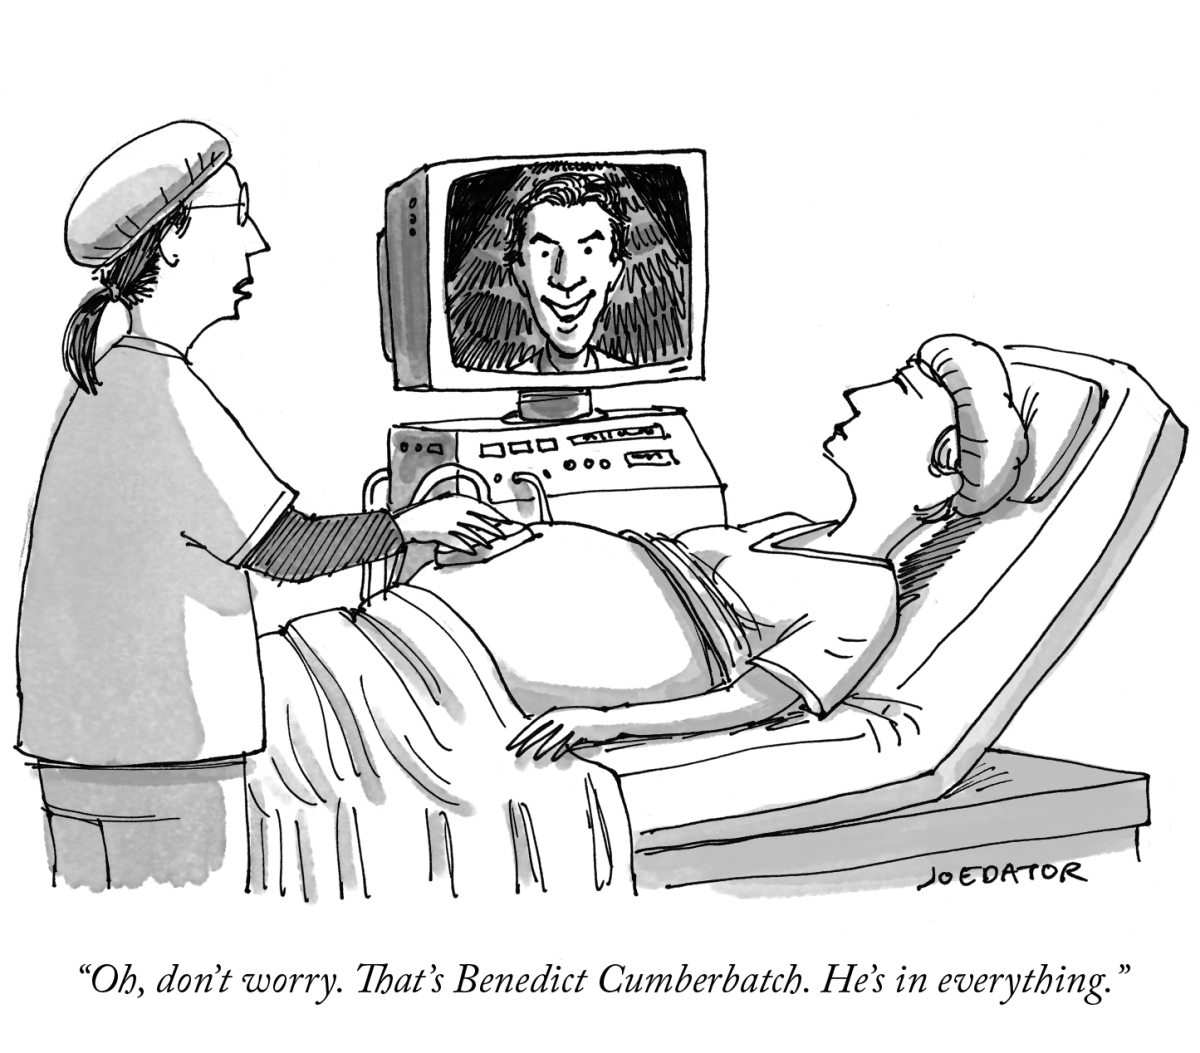
\includegraphics[width=9cm]{cartoon1.png}
\end{center}




\sektion{Number Systems}

\begin{quote}
It really seems almost obscene to go to such a higher layer of pure thought to discuss something as basic as this; but you're mathematicians, you probably look like real weirdos to all your friends, so you can rise to this.  
\begin{flushright}
      \textit{ -  Alessio Corti}
       \end{flushright} 
\end{quote}\vspace*{15pt}


Today \lecturemarker{6}{5 Oct} I take $\N, \Z$ for granted and discuss in some depth $\Q$ (and, a bit, $\R$). 

\subsektion{$\Q$, the Rationals}

Basically, elements of $\Q$ (the rational numbers) are ``things" that you write in the form: $x = m/n$, where $m \in \Z$ and $m \iN, n \neq 0$. There is a catch, and it is that $x$ cannot be uniquely written in this form: 
$2/3\; ``=" \;4/6\; ``=" \;6/9$. This is not a \emph{major} problem: $m = cm'$, $n = cn'$ with $c = \hcf(m,n)$ then the expression for $x$: $x = m'/n'$ is unique. But it is a small problem nonetheless.\\

\begin{definition}
The \emph{cartesian product} of two sets, $A,B$ is 
\[A \times B = \{(a,b) ~|~ a \in A, b \in B\}\]	
\end{definition}

Consider the Cartesian product $\Z \times (\Z \backslash\{0\})$. An element is an ordered pair $(m,n)$ where $m \in \Z$, $n \in \Z\backslash\{0\}$. (think of $(m,n)$ as a ``pedantic" way to start thinking about the fraction $m/n$.)\\

\begin{definition}
$(m,n)$ is equivalent to $(M,N)$, written as $(m,n) \sim 	(M,N)$. If $\exists a,b \in \Z\backslash\{0\}$ such that $am = bM$ and $am = bN$. 
\end{definition}

Properties of equivalence: 
\begin{enumerate}
\item $x \sim x$
\item $x \sim y \implies y \sim x$
\item $(x\sim y)$ and $(y \sim z) \implies x \sim z$	
\end{enumerate}
\emph{Exercise}: Prove this.\\

\begin{definition}
If $(m,n) \in \Z \times (\Z \backslash\{0\})$ then the \emph{equivalence class} of $(m,n)$ is the set 
\[[m,n] = \{(M,N) ~|~ (m,n) \sim (M,N)\}\]
\end{definition}

Alternative notation: $[m,n] = m/n$\\

\begin{definition}
\[\Q = \{[m,n] ~|~ (m,n) \in \Z \times (\Z \backslash\{0\})\}\]	
\end{definition}
Elements $x \iQ$ are written as ``equivalence classes" $m/n$ and now it makes perfect sense to write $2/3 = 4/6 = 6/9$.

\subsubsektion{Binary operations on $\Q$}
Suppose $(p,q)$ and $(m,n) \in \Z \times \Z\backslash\{0\}$. Then 
\[
\begin{aligned}
  (p,q) \widetilde{+} (m,n) &= (pn + qm, qn + pm)\\
  (p,q) \widetilde{\times} (m,n) &= (pm, qn)
\end{aligned}
\]


Suppose $(p,q) \sim (P,Q)$ and $(m,n) \sim (M,N)$. Then
\[
\begin{aligned}
  (p,q) \widetilde{+} (m,n) &\sim (P,Q) \widetilde{+} (M,N)\\
  (p,1) \widetilde{\times} (m,n) &\sim (P,Q) \widetilde{\times} (M,N)
\end{aligned}
\]
This shows that I can use $\widetilde{+}, \widetilde{\times}$ to define operations of equivalence classes: 
\[
\begin{aligned}
  p/q + m/n &= pn + qm/qn\\
  p/q \times m/n &= pm / qn
\end{aligned}
\]

\begin{axiom}[Axioms of $K = \Q, K = \R$]
\begin{enumerate}
\item $a + b = b + a \quad \forall a,b \in K$ ($+$ is \emph{commutative})
\item $a \times b = b \times a \quad \forall a,b \in K$	
\item $a + (b+c) = (a+b) + c$ ($+$ is \emph{associative})
\item $a \times (b \times c) = (a\times b)\times c$
\item $a \times (b + c) = (a\times b ) + (a\times c)$ ($\times$ is \emph{distributive} over $+$)
\item $\exists\, 0 \in K: a + 0 = a \quad \forall a \in K$
\item $\exists\, 1 \in K, 0 \neq 1: a \cdot 1 = a \quad \forall a \in K$
\item $\forall a \in K, \exists (-a) \in K$ such that $a + (-a) = 0$
\item $\forall a \in K \backslash\{0\} (= K^{\times}), \exists (a^{-1})$ such that $a \times (a^{-1}) = 1$. 	
\end{enumerate}\vspace*{5pt}

$\R$ satisfies an additional axiom
\begin{enumerate}
\item[(x)] Completeness axiom (I will talk about this later in the course)	
\end{enumerate}
\end{axiom}\vspace*{5pt}


\textbf{Notation:} \lecturemarker{7}{5 Oct} $a + (-b) = a-b$, and $a \times (b^{-1}) = a/b$.\\

\begin{axiom}[Trichotomy axiom]
The binary relations $<, =, >$ are such that 
\[\forall x \in K \begin{cases}
 \text{either } &x > 0 \\
 \text{or } &x = 0\\
 \text{or } &x < 0	
 \end{cases}
\]	
and only one of these conditions holds.
\end{axiom}
We then have: 
\[
\begin{aligned}
  x > 0 &\iff -x < 0\quad \forall x \in K\\
  x > 0 &\implies a + x > a \quad \forall a \in K\\
  x > 0 &\implies a \times x > 0 \quad \forall a > 0
\end{aligned}
\]

These axioms are not on the exam - it's just an intellectual exercise. We can deduce anything about $\N, \Z, \Q, \R$ from just these axioms. (BUT it can be awkward sometimes). \\

\begin{examples}
\begin{itemize}
\item[(1)] $0 \times x = 0\quad \forall x \in K$
\begin{proof} First note that:
\[(0 + 1) \cdot x = 1\cdot x = x\]
\[0 \cdot x + 1\cdot x = 0 \cdot x + x\]
So $x = 0 \cdot x + x \quad \forall x$
\[
\begin{aligned}
  (-x) + x &= (-x) + (0\cdot x + c)\\
  &= (-x) + (x + 0\cdot x) \quad  &[\text{Axiom (i)}]\\
  &= (-x + x) + 0\cdot x \quad &[\text{Axiom (iii)}]\\
  &= 0 + 0\cdot x \quad &[\text{Axiom (viii)}]\\
  &= 0\cdot x + 0 \quad &[\text{Axiom (i)}]\\
  &= 0\cdot x \quad &[\text{Axiom (vi)}]
\end{aligned}
\]
So $0 = 0\cdot x$. 
\end{proof}\vspace*{5pt}

\item[(2)] $\forall x \in K = \Q$ or $\R$, we have either $x = 0$ or $x^2 > 0$ (but never both)
\begin{proof}
There are 3 cases: 
\begin{enumerate}
\item $x = 0$ - nothing to do
\item $x >  0 \implies x\cdot x > 0$ (not much to do)
\item $x < 0 \implies -x > 0 \implies (-x) \cdot (-x) > 0$. All I need is to show that $(-x)(-x) =x\cdot x$	
\end{enumerate}\vspace*{5pt}

First I claim that $-x = (-1)\times x$ for all $x$. Indeed: 
\[
\begin{aligned}
  0 = 0\cdot x = (1 + (-1))x &= x + (-1)\cdot x\\
  -x + 0 = -x &= -x + x + (-1)\\
  &= 0 + (-1)\cdot x\\
  &= (-1)\cdot x
\end{aligned}
\]

Secondly, I claim $(-1)\cdot(-1) = 1$ (Exercise!), then I can finish (2):

\begin{align*}
  (-x)\cdot(-x) &= (-1)\cdot x \cdot (-1)\cdot x\\
  &= (-1)\cdot (-1)\cdot x\cdot x\\
  &= 1\cdot x\cdot x = x \cdot x\qedhere
\end{align*}
\end{proof}	
\end{itemize}
\end{examples}\vspace*{10pt}


\begin{example} \lecturemarker{8}{30 Oct}
Show that $\sqrt{6} - \sqrt{2} > 1$\\

Remark: If $A, B \in \R,$ \& $A,B \geq 0$, then $A >B \iff A^2 > B^2$ \\(\emph{Exercise:} show this from the axioms)\\

Write $\sqrt{6} - \sqrt{2} > 0 $; indeed $\sqrt{6} > \sqrt{2} \iff (\sqrt{6})^2 > (\sqrt{2})^2 \iff 6 > 2$\\

So 
\[\begin{aligned}
 &\sqrt{6} - \sqrt{2} > 1\\
&\iff (\sqrt{6} - \sqrt{2})^2 > 1^2 \\
& \iff 6 + 2 - 4\sqrt{3} > 1 \\
&\iff 7 > 4\sqrt{3} \\
& \iff (\frac{7}{4})^2 > (\sqrt{3})^2 \\
& \iff \frac{49}{16} > 3 \\
& \iff 49 > 48 \\
& \iff 1 > 0
\end{aligned}\]which follows from the axioms. 
\end{example}\vspace*{10pt}

\begin{example}
Is $\sqrt{2} + \sqrt{3} > \sqrt{10}$? 
\[
\begin{aligned}
  &\sqrt{2} + \sqrt{3} > \sqrt{10} \\
  &\iff (\sqrt{2} + \sqrt{3})^2 > (\sqrt{10})^2 \\
  &\iff 5 + 2\sqrt{6} > 10 \\
  &\iff \sqrt{6} > \frac{5}{2}\\
  &\iff 6 > \frac{25}{4} \\
  &\iff 24 > 25 \\
  &\iff 0 > 1, \text{ which is false. So the answer is no.}
\end{aligned}
\]
\end{example}\vspace*{10pt}

\begin{example}
Solve $x > \dfrac{2}{x+1}$ for $x \in \R$ [$x + 1 = 0 \implies$ RHS makes no sense] \\

Cases: \begin{enumerate}
 \item[(i)]$x + 1 > 0$ 
 \item[(ii)] $x+1<0$ 
 \end{enumerate}

 Starting with (i):
\begin{align*}
   x(x+1) > 2 &\implies x^2 - x - 2 >0\\
   &\implies (x-1)(x+2)>0
\end{align*}
 Recall $x > -1$, so case (i) $\implies x \in (1,\infty) = \{x \;|\; 1 < x\}$\\
 
 Next (ii):
\begin{align*}\\[-1cm]
   x(x+1) <2 &\implies x^2 - x - 2 < 0\\
   & \implies (x-1)(x+2) < 0
\end{align*}
 Then $x \in (-2,1) \cap (-\infty,-1) = (-2,-1)$. So our final answer is:
\[x \in (-2,-1) \cup (1,\infty)\]
\end{example}\vspace*{10pt}


\begin{definition}[Absolute Value Function]
\[|x| = \begin{cases}
 x & \text{if } x \geq 0\\
 -x &\text{if } x < 0
 \end{cases}\]
 (so $|x| \geq 0\quad \forall x\in K$)
 \end{definition}

\emph{Exercise:} Solve for $x \iR$: $|x+4| < |x-5|$, do it properly! (hint: $|x| < A \iff -A < x < A$)


\subsektion{$\R$, the Real Numbers}

A remarkable  \lecturemarker{9}{30 Oct}thing: $\Q \neq \R$. For example: $\sqrt{2} \not\in \Q$. 

Do we know for sure that $\sqrt{2}$ exists? i.e. $\exists x \iR$ such that $x \geq 0$ and $x^2 =2$. We will answer this analyst-style later in the course. The geometer-style makes this obvious: 
\begin{center}
\begin{tikzpicture}
	\draw (0,0) rectangle (2,2);
	\draw (0,0) -- (2,2); 
	\node at (1,-0.3) {$1$};
	\node at (-0.3,1) {$1$};
	\node at (0.9,1.3) {$\sqrt{2}$};
\end{tikzpicture}	
\end{center}

I can prove: $x \in \Q \implies x^2 \neq 2$. 
\begin{proof}
Define $x = p/q$ with $p \in \Z$ and $q\in \Z$ are both are not even. 

Suppose for contradiction that $x^2 = 2$. Then $p^2 = 2q^2$. $p$ must be even, so $p = 2p'$ and $4p'^2 = 2q^2$. Then $q^2 = 2p'^2$. So $q$ is also even: a contradiction. 
\end{proof}

\emph{Exercise:} $\sqrt{3} \not \in \Q$ ($3$-adic argument using divisibility by $3$)\\

\textbf{Claim:} $\sqrt{2} + \sqrt{3} \not \in \Q$. 
\begin{proof}
	Assume for contradiction $r = \sqrt{2} + \sqrt{3} \in \Q$. Then 
	\[
\begin{aligned}
  r^2 &= (\sqrt{2} + \sqrt{3})^2 = 5 + 2\sqrt{6} \in \Q\\
  \implies \sqrt{6} &= \frac{r^2-5}{2} \in \Q 
\end{aligned}
\]
but $\sqrt{6} \not \in \Q$: If $\sqrt{6} = p/q$, we may assume $p,q$ are not both even, then $p^2 = 6q^2$, so $2 \divides p$ and $4p'^2 = 6q^2$. Then $3q^2 = 2p'^2 \implies q$ is also even, a contradiction. 
\end{proof}

\emph{Exercise:} Let $x \iR$. Prove there is a unique $N \in \Z$ such that $N \leq x < N+1$. $N$ is called the \emph{round down} of $x$ and is denotes $N: \lfloor x \rfloor$

[hint: assume $x \geq 0$, then  consider $S = \{n \iN ~|~ n > x\} \subset \N$. Note by the Archimedean axiom $S$ has a smallest element. Claim: $\lfloor x \rfloor = -1 + $ smallest element $(S)$.]


\subsubsektion{Decimal Expansions of Reals}
You are all familiar with the
\[\frac{1}{9} = 0.1111\dots = 0.\overline{1}\]\vspace*{5pt}

\emph{How can we really make sense of this?}
\[
\begin{aligned}
  \frac{1}{9} &= 0.1 + 0.01 + 0.001 + 0.0001 + \dots\\
  &= \frac{1}{10} + \frac{1}{100} + \frac{1}{1000} + \frac{1}{10000} + \dots\\
  &= \; ? \\
  &= \frac{1}{10}\left(1 + \frac{1}{10} + \left(\frac{1}{10}\right)^2 + \left(\frac{1}{10}\right)^3 + \dots \right)\\ 
  &= \frac{1}{10} \cdot\frac{1}{1-\frac{1}{10}} = \frac{1}{10}\frac{10}{9} = \frac{1}{9}
\end{aligned}
\]\vspace*{5pt}

\begin{remark}
\[1 + x + x^2 + \dots + x^n = \frac{1-x^{n+1}}{1-x}\]
If $-1 < x < 1$ then 
\[
\begin{aligned}
  1 + x + x^2 + \dots + x^n + \dots &= \lim_{n\to \infty}\frac{1-x^{n+1}}{1-x}\\
  &= \frac{1}{1-x}
\end{aligned}
\]
For now let's agree that all of this makes sense. 
\end{remark}


\begin{theorem} \lecturemarker{10}{30 Oct}
$\forall x \iR, \;\exists!\,n \iZ : n \leq x < n+1$. We write $n = \lfloor x \rfloor$, the \emph{integer part} of $x$. The \emph{fractional part} of $x$ is $\{x\} = x - \lfloor x\rfloor$, where $0 \leq \{x\} < 1$. 	
\end{theorem}\vspace*{5pt}

\begin{corollary}[Euclid's Algorithm]
	Let $p \iZ,\, q \iN\backslash\{0\}$. Then $\exists a \iZ,\, r \iN$ with 
	$p = qa + r \text{ and } 0 \leq r < q$. 
\end{corollary}
\begin{proof}
Take $a = \lfloor \frac{p}{q}\rfloor$. Then $\frac{p}{q} = a + f$ where $f = \{\frac{p}{q}\}$. Let $r = qf$. Note that $r \iZ$; indeed $r = qf = p-qa \iZ$. Also $0 \leq f < 1 \implies 0 \leq r = qf < q.$ 	
\end{proof}

We will come back to this later in the course. Today I use this to understand decimal expansions. We consider decimal expansions: 
\[x = a_0 . a_1a_2a_3 \dots \qquad (*)\]
where $a_0 \iZ$ and $a_1,a_2,a_3,\dots$ are digits $0 \leq a_i \leq 9$ for all $i$. 

I take $(*)$ to mean: 
\[x = a_0 + \frac{a_1}{10} + \frac{a_2}{10^2} + \dots + \frac{a_n}{10^n}+ \dots\]

\begin{theorem}
Every $x\iR$ has a decimal expansion. 	
\end{theorem}

\begin{proof}
Let $x\iR$. We can construct the decimal expansion of $x$: 

$\exists M \iZ : M \leq x < M+1$ ($M$ is the \emph{round down} of $x$, denoted $\lfloor x \rfloor$). 

We start with $a_0 = M = \lfloor x \rfloor$ and write: 
\[[a_0, a_0+1) = [a_0,a_1 + \frac{1}{10}) \cup [a_0 + \frac{1}{10}, a_0+\frac{2}{10})\cup \dots\cup [a_0 + \frac{9}{10},a_0 + 1)\]	

Clearly there is a unique $a_1 \in \{0,1,\dots,9\}$ such that $x \in [a_0, \frac{a_1}{10} + a_0 + \frac{a_1 + 1}{10})$. This constructs $a_1$. Continue to do this for $a_2$ etc. We have a procedure that inductively determines all of the decimal expansion of $x$. 
\end{proof}\vspace*{5pt}

\begin{example}
$2/7 = 0.\overline{285714}$, using long division. 
\[
   \opdiv[period]{2}{7}
\]

\end{example}

In summary let $x \iR$. Then $x = a.a_1a_2a_3a_4\dots$ with $a,a_k \in \Z$ and $0\leq a_k \leq 9$, where $a = \lfloor x \rfloor$ and $a_k (k \geq 1)$ are defined inductively, starting from $f_0 = \{x\}$ by $a_{k+1} = \lfloor 10f_k\rfloor$ where $f_k = \{10f_{k-1}\}$.\\

\begin{theorem}
Let $x \iR$. Then $x \iQ \iff$	the decimal expansion of $x$ is eventually periodic, i.e. $x = a. a_1\dots a_n \overline{b_1\dots b_k}$
\end{theorem}\vspace*{5pt}

\begin{example}
	$x = 0.1010010001\dots \not \in \Q$. 
\end{example}

Point to take home: the theorem provides a very large supply of explicit, easily described irrational numbers. 

\begin{proof}
$\impliedby$: If the decimal expansion is eventually periodic, then $x\iQ$:
\[x = a.a_1\dots a_n +\frac{1}{10^n}(0.\overline{b_1\dots b_k})\]

It is enough to show that $y = 0.\overline{b_1\dots b_k} \iQ$:
\[
\begin{aligned}
  y &= b_1\dots b_k\left(\frac{1}{10^k} + \frac{1}{10^{2k}} + \frac{1}{10^{3k}} + \dots \right)\\
  &= \frac{b_1\dots b_k}{10^k} \frac{1}{1-\frac{1}{10^k}} \in \Q.
\end{aligned}
\]

Next I prove $\implies$:

 Assume $x = p/q \iQ$, where $p \iZ, q \iZ, q \geq 1$. Then the expansion is eventually periodic: $x = p/q \iQ$. Let $a = \lfloor x \rfloor$, $f = \{x\}$, so by the division theorem $p = aq + r$ where $r = qf$. 

Inductively we calculate: 

$a_1 = \lfloor 10f\rfloor, f_1 = \{10f\}$, so $10r = a_1q + r_1$ where $r_1 =qf_1$. 

$a_2 = \lfloor 10f_1\rfloor, f_2 = \{10f_1\}$, so $10r_1 = a_2q + r_2$ where $r_2 = qf_2$. 

\hspace*{5cm} $\vdots$

$a_k = \lfloor 10f_{k-1}\rfloor, f_k = \{10f_{k-1}\}$, so $10r_{k-1} = a_kq + r_k$ where $r_k = qf_k$. 

\hspace*{5cm} $\vdots$\\


In other words: write $p = aq + r$, then define $r_k (k \geq 1)$, $a_k$ inductively by: $10r_{k-1} = a_kq + r_k\quad 0 \leq r_k \leq 9$. 
(the process / construction guarantees that $0\leq a_k \leq 9$). Because $0 \leq r_k < 9$ for all $k$, at some point $r_n = r_m,\; n > m$. This means that $x = a.a_1 \dots \overline{a_m\dots a_{n-1}}$, that is the decimal expansion is eventually periodic. 
\end{proof}

Non-uniqueness of decimal expansions:  \lecturemarker{11}{30 Oct}
\[
\begin{aligned}
  0.9999 \dots &= 0.\overline{9} = 1\\
  &= \frac{9}{1} + \frac{9}{100} + \dots \\
  &= \frac{9}{10}\left( 1 + \frac{1}{10} + \left(\frac{1}{10}\right)^2 + \dots + \left(\frac{1}{10}\right)^n + \dots \right)\\
  &= \frac{9}{1} \cdot \frac{1}{1 -\frac{1}{10}} = \frac{9}{10} \times \frac{10}{9} = 1
\end{aligned}
\]\vspace*{5pt}

\begin{proposition}
Suppose $x\iR$ has two different decimal expansions. Then these are as follows: 
\[
\begin{aligned}
  x &= a_0 . a_1a_2\dots a_n \overline{9}\\
  &= a_0. a_1a_2\dots (a_{n} + 1) \quad (0 \leq a_n \leq 8)
\end{aligned}
\]
\end{proposition}

\begin{proof}
Suppose the two expansions are:
\[
\begin{aligned}
  x &= a_0 . a_1 a_2 \dots a_n a_{n+1} \dots\\
  &= a_0 . a_1 a_2 \dots b_n b_{n+1} \dots 
\end{aligned}
\]
with $a_n < b_n$. Then: 
\[
\begin{aligned}
   x &= a_0 . a_1 a_2 \dots a_n a_{n+1} \dots \\
   &\leq a_0 . a_1a_2 \dots a_2 999\dots\\
   &= a_0 . a_1a_2 \dots (a_{n} + 1) 000\dots\\
   &\leq a_0 . a_1 a_2 \dots b_n b_{n+1} \dots \\
   &= x
\end{aligned}
\]

So all $\leq$ must have been $=$ and this shows the proposition. 
\end{proof}

\textit{Exercise:} $\forall x,y \iR, x < y$ show that 
\begin{enumerate}
\item $\exists z \iQ: x < z < y$
\item $\exists 	z \not \in \Q: x < z < y$
\end{enumerate}\vsp

%skipped blue part of p52.



\subsubsektion{Rational Powers}
Later in the year you will see the proof of the following: 
\begin{theorem}[Existence of $n$-th root] 
$\forall n \iN \backslash \{0\}$, $\forall x \iR$, $x \geq 0$, $\exists!\, y \iR,\, y \geq 0: y^n = x$. 	
\end{theorem}

\textbf{Notation:} $y = \sqrt[n]{x} = x^{\frac{1}{n}}$. 

Today we take the theorem for granted and draw some consequences. \\

\begin{definition}
For $r = p/q \geq 0$ and $x \iR$, $x \geq 0$ we define $x^r = \left(x^{\frac{1}{q}}\right)^p$.	
\end{definition}

\begin{remark} $x^r$ is well-defined. Recall $p/q = p'/q'$. Iff $\exists m,n$ such that $mp = np'$ and $mq = nq'$. To show $x^r$ is well defined, it is enough to show that $(x^{\frac{1}{q}})^p = ( x^{\frac{1}{mq}})^{mp}$. We'd like to do $(x^{\frac{1}{q}})^p = x^{\frac{mp}{mq}} = x^{\frac{p}{q}} =( x^{\frac{1}{mq}})^{mp}$, 
but this is using precisely the thing that we want to prove.

\begin{proof}
\[
\begin{aligned}
    \left(x^{\frac{1}{q}}\right)^p &= \left(\left(x^{\frac{1}{mq}}\right)^m\right)p \\
    \iff x^{\frac{1}{q}} &= \left(x^{\frac{1}{mq}}\right)^m\\
    \iff x &= \left( x^{\frac{1}{mq}}\right)^{mq} 
\end{aligned}
\]
and this is true by definition of $x^{\frac{1}{mq}}$
\end{proof}
\end{remark}


Properties: Suppose $\alpha, \beta \in \Q_{\geq 0}$, and $x,y \in \R_{\geq 0}$. Then 
\begin{enumerate}
\item $x^\alpha x^\beta = x^{\alpha + \beta}$
\item $x^{\alpha} y^{\alpha} = (xy)^{\alpha}$
\item $(x^\alpha)^\beta = x^{\alpha \beta}$
\end{enumerate}

\begin{proof} (i) Assume the result for integer powers. 
\[
\begin{aligned}
  x^\alpha x^\beta &= \left(x^{\frac{1}{n}}\right)^m \left(x^{\frac{1}{q}}\right)^p\\
  &= \left(x^{\frac{1}{nq}}\right)^{mq} \left(x^{\frac{1}{nq}}\right)^{np}\\
  &= \left(x^{\frac{1}{nq}}\right)^{mq + np}
\end{aligned}
\]
by what we just did. By results on integer powers this is $x^{\frac{mq + np}{nq}} = x^{\alpha + \beta}$. 
\end{proof}
\emph{Exercise:} (ii) and (iii).



\subsektion{$\C$, the Complex Numbers} 


Consider 
\[\R^2 = \R \times \R:= \{(a,b): a \iR, b\iR\}\]

(the symbol $:=$, ``colon equal" means LHS is defined to be RHS)\\

\begin{definition} We define operations on $\R^2$: 
\[
\begin{aligned}
  (a,b) + (c,d) &:= (a+c,b+d)\\
  (a,b) \cdot (c,d) &:= (ac-bd, ad+bc)
\end{aligned}
\]
The two operations satisfy all of the axioms for $K = \R, \Q$ except anything to do with $<, >$. We call $\R^2$ together with $+$ and $\cdot$ as $\C$. 
\end{definition}

We think of $\R$ as a subset of $\C$: 
\[\R \ni x \longmapsto (x,0) \in \C\]
we write $i = (0,1)$. Then we can write every element $(a,b) \iC$ uniquely as
\[
\begin{aligned}
  (a,b) &= (a,0) + (0,b)\\ 
  &= (a,0) + (0,b)(0,1)\\
  &= (a,0) + i(0,b)\\
  &= a + ib
\end{aligned}
\]
and we call this the Cartesian form of the complex numbers $(a,b)$. 

You picture the complex numbers on the Cartesian plane: 

\begin{center}
\begin{tikzpicture}[scale=0.9]
	\draw[->] (-3,0) -- (3,0) node at (2.8, -0.3) {$\Re$};
	\draw [->] (0,-1) -- (0,3) node at (-0.3,2.8) {$\Im$};
	\draw[dashed] (0,2) -- (2,2) node at (2.4,2.4) {$(a,b) = a+ib$};
	\draw[dashed] (2,0) -- (2,2);
	\draw (1,-0.05) -- (1,0.05) node at (1.1,-0.2) {$1$};
	\draw (-0.05,1) -- (0.05,1) node at (-0.2,1.1) {$i$};	
	\fill (2,2) circle (2pt);
\end{tikzpicture}	
\end{center}

Note that addition in $\C$ is the addition of vectors in $\R^2$. 

Now $i^2 = (0,1)^2 = (0,1)\cdot (0,1) = (-1,0) = -1$, so using the properties (axioms) we have: 
\[
\begin{aligned}
   (a+ib)(c+id) &= ac +ibc + aid + ibid &\quad\text{(distributive property)}\\
   &= ac + i^2bd + ibc + iad &\quad\text{(commutative property)}\\
   &= (ac - bd) + i(bd + ad) &\quad\text{(associative property)}
\end{aligned}
\]

This is familiar and it motivates the definition we started out with.

%\textbf{More terminology and notation}

If  \lecturemarker{12}{30 Oct} $z = a + ib \in C$ ($a,b \iR$), then we denote $\bar{z} := a-ib$ as the \emph{complex conjugate} of $z$.

\begin{center}
\begin{tikzpicture}
	\draw[->] (-3,0) -- (3,0) node at (2.8, -0.3) {$\Re$};
	\draw [->] (0,-1.5) -- (0,2) node at (-0.3,2) {$\Im$};
	\draw (1,-0.05) -- (1,0.05) node at (1.1,-0.2) {$1$};
	\draw (-0.05,1) -- (0.05,1) node at (-0.2,1.1) {$i$};	
	\fill (2,1.2) circle (2pt) node at (2.4,1.2) {$z$};
	\fill (2,-1.2) circle (2pt) node at (2.4,-1.2) {$\bar{z}$};	
\end{tikzpicture}	
\end{center}

Conjugation is reflection in the real axis.\\

If $z = a + ib \iC$ ($a,b \iR$) then: 
\begin{itemize}
\item $a =$ real part of $z$, denoted $\mathrm{Re}(z)$
\item $b = $ imaginary part of $z$, denoted $\mathrm{Im}(z)$	
\end{itemize}\vspace*{5pt}

So $z = \mathrm{Re}(z) + i\,\mathrm{Im}(z)$. Notice that \[\mathrm{Re}(z) = \dfrac{z + \bar{z}}{2},\,
\mathrm{Im}(z) = \dfrac{z-\bar{z}}{2i}\]

We denote $|z|:= \sqrt{a^2 + b^2} = \sqrt{z\bar{z}}$ as the \emph{absolute value} of $z\iC$. (note that if $z = a +ib$, then $z\bar{z} = (a+ib)(a-ib) = a^2+b^2$.)\\


\subsubsektion{Properties of the absolute value of complex numbers}
\begin{enumerate}
\item $|z| \geq 0$ and $|z| = 0 \iff z = 0$
\item If $\lambda \iR$, then $|\lambda z| = |\lambda||z|$
\item $|z+w| \leq |z| + |w|$ (triangle inequality)	
\end{enumerate}\vsp

\textbf{Question:} \emph{Why is (iii) called the triangle inequality?}

 First understand $z + w$ in terms of the parallelogram law: 
\[(a+ ib) + (a' + ib') = a + a' + i(b + b')\]
i.e. 
\[\begin{pmatrix}
a \\ b	
\end{pmatrix}
+ \begin{pmatrix}
 a' \\ b'	
 \end{pmatrix}
= \begin{pmatrix}
 a + a'\\ b + b'	
 \end{pmatrix}
\]


\begin{center}
\begin{tikzpicture}
	\draw[->] (-3,0) -- (3,0) node at (2.8, -0.3) {$\Re$};
	\draw [->] (0,-1) -- (0,2.5) node at (-0.3,2.8) {$\Im$};
	\draw (1,-0.05) -- (1,0.05) node at (1.1,-0.2) {$1$};
	\draw (-0.05,1) -- (0.05,1) node at (-0.2,1.1) {$i$};	
	\fill (2,0.8) circle (2pt) node at (2.4,0.9) {$z$};
	\fill (0.5,1.8) circle (2pt) node at (0.4,2.1) {$w$};
	\draw [->] (0,0) -- (0.5,1.8);
	\draw [->] (0,0) -- (2,0.8);
	\draw [dashed] (0.5,1.8) -- (2.5,2.6);
	\draw [dashed] (2,0.8) -- (2.5,2.6) node at (2.7,2.7) {$z + w$};
	\draw [->] (0,0) -- (2.5,2.6);
\end{tikzpicture}	
\end{center}

Secondly, we have an interpretation: $|z| = \text{distance}\,(0,z) = $ distance. The triangle inequality is the obvious fact that the two sides of any triangle (on the Euclidean plane) must be greater than or equal to the other side. 

Also note: $|z| \geq 0$ and $0$ iff $z = 0$. So if $z \neq 0$, then $1 = \dfrac{z\bar{z}}{|z|^2}$. That is, \[z^{-1} = \dfrac{\bar{z}}{|z|^2}\] 


\begin{example}
	Express $\dfrac{1 +i}{1 - 2i}$ in Cartesian form:
	
	\[
\begin{aligned}
  \frac{1+i}{1-2i} &= \frac{1 +i}{1 - 2i} \times \frac{1 + 2i}{1 + 2i}\\[0.3cm]
  &= \frac{(1-2) + (2 + 1)i}{5}\\[0.3cm]
  &= \frac{-1}{5} + \frac{3i}{5}
\end{aligned}
\]

\end{example}




\subsubsektion{Polar form of complex numbers}


(Motivation: the polar form allows us to neatly visualise complex multiplication much in the same way as the Cartesian form allows us to visualise complex addition.) 

\begin{center}
\begin{tikzpicture}[scale = 0.65]
\draw[->] (-2.5,0) -- (2.5,0) node at (2.5,-0.3) {$\Re$};
\draw[->] (0,-2.5) -- (0,2.5) node at (-0.3,2.5) {$\Im$};
\draw (0,0) circle (2);
\draw[->] (0,0) -- (1, 1.73) node at (2, 2.1) {$z = a + ib$};
\draw (0.5, 0) arc (0:40:0.8);
\node at (0.6, 0.4) {$\theta$};
\end{tikzpicture}
\end{center}

$z$ lies on a circle of radius $r = |z|$ and $\theta = $ angle from $\R$ to $z$. The polar form of $z$ is in terms of data $(r,\theta)$. \\

\begin{definition}[Euler's form]
 If $\theta \iR$ then we write 
 \[e^{i\theta} := \cos \theta + i\sin\theta\]
\end{definition}

\emph{How can we motivate this? }

\begin{enumerate}
\item It just works: $e^{i(\theta_1 + \theta_2)} = e^{i\theta_1} + e^{i\theta_2}$ because
\[
\begin{aligned}
  e^{i(\theta_1 + \theta_2)} &:= \cos(\theta_1 + \theta_2) + i\sin(\theta_1 + \theta_2)\\
  &= (\cos\theta_1\cos\theta_2 - \sin\theta_1\sin\theta_2) + i(\sin\theta_1\cos\theta_2 + \sin\theta_2\cos\theta_1)\\
  &= (\cos\theta_1 + i\sin\theta_1)(\cos\theta_2 + i\sin\theta_2)
\end{aligned}
\]
In otherwords, the trig identities allow us to generalise the exponential function to a function of a complex variable: 
\[e^z = e^{x + iy} := e^x (\cos y + i\sin y)\]
while preserving the usual property 
\[e^{z_1 + z_2} = e^{z_1} e^{z_2}\]

\item There are other considerations - you may be familiar with the infinite series for the exponential; if $x \iR$, then 
\[e^x = 1 + x + \frac{x^2}{2!} + \frac{x^3}{3!} + \dots \]
\emph{Could it just be that this makes sense for complex numbers?}
\[
\begin{aligned}
 e^{i\theta} &= 1 + i\theta - \frac{\theta^2}{2!} - \frac{i\theta^3}{3!} + \frac{\theta^4}{4!} + \dots\\
 &= \left( 1 - \frac{\theta^2}{2!} + \frac{\theta^4}{4!} - \frac{\theta^6}{6!} + \dots\right) + i\left( \theta - \frac{\theta^3}{3!} + \frac{\theta^5}{5!} - \dots\right)\\
 &= \cos\theta + i\sin\theta.
\end{aligned}
\]
\end{enumerate}

I gave some motivation for the formula
$e^{i\theta} = \cos\theta + i\sin\theta$. Please now accept this. Thus, $e^{i\theta} = z$ is the complex no. $z$ with $|z| = \cos^2 \theta + \sin^2\theta = 1$ and angle $\theta$ from the $\R$-axis to $z$: 

\begin{center}
\begin{tikzpicture}[scale= .7]
\draw (-3,0) -- (3,0) node at (2.9,-0.2) {$\Re$};
\draw (0,-2.5) -- (0,2.5) node at (-0.2,2.5) {$\Im$};
\draw (0,0) circle (2);
\draw[->] (0,0) -- (1, 1.73) node at (1.2,1.9) {$z$};
\draw[->] (0.5, 0) arc (0:40:0.8);
\node at (0.6, 0.4) {\small $\theta$};
\node at (2.1,-0.3) {$1$};
\fill (2,0) circle (2pt);
\node at (2.22,1.3) {\small $|z|\;\;=\; \sqrt{x^2 + y^2} = 1$};
\end{tikzpicture}
\end{center}


Then every $z = x + iy \iC$ can be written uniquely if $z \neq 0$ in the polar form $z = re^{i\theta}$ for $r = |z| = \sqrt{x^2 + y^2} \iR_{\geq 0}$ and $\theta$ as an angle $\in (-\pi,\pi]$, where I call $r$ the \emph{modulus} of $z$ and $\theta = \mathrm{arg}(z)$, the \emph{argument}. 

Conversion formulas: 
\[\begin{cases}
x &= r\cos\theta\\
y &= r \sin\theta\\
\end{cases}
\qquad 
\begin{cases}
r &= \sqrt{x^2 + y^2}\\
\tan \theta &= \frac{y}{x}
\end{cases}
\]

Note: our formula for $\theta$ does not nail it down uniquely; we need to make sure that $\theta \in (-\pi,\pi]$ is in the correct quadrant.\\

\begin{theorem}[De Moivre's Formula]
If $z_1 = r_1e^{i\theta_1} \iC$ and $z_2 = r_2 e^{i\theta_2}\iC$ then 
\[z_1 \cdot z_2 = r_1 r_2 e^{i(\theta_1 + \theta_2)}\]
\end{theorem}

Basically: modulus' multiplies; arguments add. This allows us to visualise multiplication by $z = r^{i\theta}$: $\C \ni w \longrightarrow z\cdot w \iC$. This is the linear transformation of $\C = \R^2$ which inflates everything by factor $r$ and rotates everything through angle $\theta$.\\


\begin{examples}
Everyone should know these complex numbers: 

\begin{minipage}{6cm}
\begin{center}
\begin{tikzpicture}[scale=.8]
\draw (-2.5,0) -- (2.5,0) node at (2.2,-0.2) {$\Re$};
\draw (0,-2) -- (0,2) node at (-0.2,2) {$\Im$};
\draw (0,0) circle (1.5);
\draw (0.5, 0) arc (0:90:0.5);
\node at (0.5, 0.5) {$\frac{\pi}{2}$};
\draw[->] (0,0) -- (0,1.5) node at (0.2,1.7) {$i$};
\end{tikzpicture}
\end{center}
\begin{center}
\begin{tikzpicture}[scale=.8]
\draw (-2.5,0) -- (2.5,0) node at (2.2,-0.2) {$\Re$};
\draw (0,-2) -- (0,2) node at (-0.2,2) {$\Im$};
\draw (0,0) circle (1.5);
\draw (0.5, 0) arc (0:45:0.5);
\node at (0.7, 0.35) {$\frac{\pi}{4}$};
\draw[->] (0,0) -- (1.05,1.05) node at (1.4,1.3) {$e^{\frac{i\pi}{4}}$};
\end{tikzpicture}
\end{center}

\begin{center}
\begin{tikzpicture}[scale=.8]
\draw (-2.5,0) -- (2.5,0) node at (2.2,-0.2) {$\Re$};
\draw (0,-2) -- (0,2) node at (-0.2,2) {$\Im$};
\draw (0,0) circle (1.5);
\draw (0.5, 0) arc (0:30:0.5);
\node at (0.9, 0.25) {$\frac{\pi}{6}$};
\draw[->] (0,0) -- (1.3,0.8) node at (1.6,1) {$e^{\frac{i\pi}{6}}$};
\end{tikzpicture}
\end{center}
\end{minipage}
\begin{minipage}{6cm}
\[i = e^{\frac{i\pi}{2}}\]

\vspace*{2.5cm}

\[\frac{\sqrt{2}}{2} + i\frac{\sqrt{2}}{2} = e^{\frac{i\pi}{4}}\]


\vspace*{2.5cm}

\[\frac{\sqrt{3} + i}{2} = e^{\frac{i\pi}{6}}\]

\end{minipage}
\vspace*{10pt}

\emph{What's $e^{\frac{i\pi}{12}}$?}

Note that $\frac{1}{4} - \frac{1}{6} = \frac{3-2}{12} = \frac{1}{12}$, so by De Moivre's formula: 
\[
\begin{aligned}
  &= \frac{\sqrt{2} + i\sqrt{2}}{\sqrt{3} + i} \times \frac{\sqrt{3} - i}{\sqrt{3} + i}\\[.2cm]
  &= \frac{(\sqrt{6} + \sqrt{2}) + i(-\sqrt{2} + \sqrt{6})}{4}\\[.2cm]
  &= \frac{\sqrt{6} + \sqrt{2}}{4} + i\frac{-\sqrt{2} + \sqrt{6}}{4}
\end{aligned}
\]


	
\end{examples}\vspace*{5pt}


\subsubsektion{Complex roots of 1}

Consider the equation \lecturemarker{13}{5}
\[z^n = 1 \quad \text{for } z \iC\]

Write $z = re^{i\theta}$, then we want $z^n = r^ne^{in\theta} = 1$. That is, $r^n = 1$ 
\[
\begin{aligned}
  \implies r &=1 \text{ and }n \theta = 2k\pi\text{ for some }k \iZ \\
   \implies \theta &= \frac{2\pi}{n} \cdot R\text{ for some }R \iZ
\end{aligned}
\]


\emph{How many solutions are there?} 

$r = 1$, so $z$ is on the circle of radius $1$. I draw the picture for $n = 12$: 

 
\begin{center}
\begin{tikzpicture}
\draw (-2.5,0) -- (2.5,0) node at (2.5,-0.2) {$\Re$};
\draw (0,-1.5) -- (0,1.5) node at (-0.2,1.8) {$e^{i3\pi/6}$};
\draw (0,0) circle (1.5);
\draw[->] (0,0) -- (-0.866*1.5, -.5*1.5) node at (1.8, 0.8) {$e^{i\pi/6}$};
\draw[->] (0,0) -- (0.866*1.5, -.5*1.5) node at (1.4, 1.6) {$e^{i2\pi/6}$};
\draw[->] (0,0) -- (-0.866*1.5, .5*1.5) node at (-1.4, 1.6) {$e^{i4\pi/6}$};
\draw[->] (0,0) -- (.866*1.5, .5*1.5) node at (-1.8, 0.8) {$e^{i5\pi/6}$};
\draw[->] (0,0) -- (-.5*1.5, -.866*1.5) node at (-1.8, -0.8) {$e^{i7\pi/6}$};
\draw[->] (0,0) -- (-.5*1.5, .866*1.5) node at (-1.4, -1.6) {$e^{i8\pi/6}$};
\draw[->] (0,0) -- (.5*1.5, .866*1.5) node at (1.4, -1.6) {$e^{10\pi/6}$};
\draw[->] (0,0) -- (.5*1.5, -.866*1.5) node at (1.8, -0.8) {$e^{i11\pi/6}$};
\draw[->] (0,0) -- (1.5,0);
\draw[->] (0,0) -- (-1.5,0);
\draw[->] (0,0) -- (0,-1.5);
\draw[->] (0,0) -- (0,1.5);


\end{tikzpicture}
\end{center}

The solutions to $z^n = 1$ ($z \iC$) are the complex numbers
\[z \in \{z = e^{i\frac{2\pi}{n}}k ~|~ k = 0,1,2,\dots,n-1\}\]

They are the vertices of a regular $n$-gon inscribed in the unit circle with a vertex at $1$. Another way to say this: Let $w = e^{i\frac{2\pi}{n}}$. Then the solutions of $z^n = 1$ are $1,w,w^2,w^3,\dots,w^{n-1}$. \\

\begin{example}
Solve for $z$, $z^n = 3$. 

We want $z = re^{i\theta}$ such that $z^n = r^ne^{in\theta} = 3 \iff r^n = 3$ and $e^{in\theta} = 1$. So
 \[z^n = 3 \iff z \in \{\sqrt[n]{3} w^k ~|~ w = e^{\frac{2\pi i}{n}}\; k = 0,1,\dots,n-1\}\]
\end{example}


%missing page 74



\subsektion{Polynomial equations}
\vspace*{10pt}
\begin{theorem}[Fundamental Theorem of Algebra]
Any polynomial with complex coefficients of degree $n \geq 1$: 
\[p(z) = a_n z^n + a_{n-1}z^{n-1} + \dots + a_0\]
($a_0,a_1,\dots,a_n \iC$, and $a_n \neq 0$) has a root $\lambda \iC$. 
\end{theorem}

In other words, there $\exists \lambda \iC$ such that $p(\lambda) = 0$.

\emph{Proof.} In the 2nd year Complex Analysis course. 

One of the most basic things in maths you learn early on is to solve the quadratic equation. The Fundamental Theorem of Algebra says that any equation of order $n$ has such a result. It is an existential result, it doesn't tell you how to find them.

 There is a formula for $n =3$ (next week), it's very complicated, and strangely useless in a deep kind of way. Then there is a formula for $n=4$, which I won't tell you as it takes half an hour to write down. For a long time people tried to find formulas for $n=5$, until in the 19th century Galois proved there is no such formula.


\begin{corollary}
Let 
\[p(z) = a_n z^n + a_{n-1}z^{n-1} + \dots + a_0\]
($a_n \neq 0$) be a complex polynomial of degree $n$. There are $\lambda_1,\lambda_2,\dots,\lambda_n \iC$ such that 
\[p(z) = a_n(z-\lambda_1)(z-\lambda_2)\dots(z-\lambda_n)\]
\end{corollary}

(the equation $p(z) = 0$ has $n$ solutions $\lambda_1,\lambda_2,\dots,\lambda_n \iC$  - perhaps counted with multiplicity). 

\begin{proof}
	This is based on the \emph{long division algorithm} for polynomials. 
	
	Consider any $\lambda \iC:$ I can write: 
	\[
\begin{aligned}
  p(z) &= a_nz^n + a_{n-1}z^{n-1} + \dots + a_0\\
  &= a_n (z-\lambda)(z^{n-1} + b_{n-2}z^{n-2} + \dots + b_0) + r
\end{aligned}
\]
where $r$ is a constant. So 
\[p_n(z) = (z-\lambda)q_{n-1}(z) + r\]

Plug in $z = \lambda$: $p_n(\lambda = r)$, so $\lambda \iC$ is a root of $p$, i.e. $p(\lambda)  = 0 \iff r = 0$. 

So let $\lambda_1 \iC$ be a root of $p(z)$ (such a thing exists by the fundamental theorem); then 
\[p_n(z) = (z-\lambda_1)q_{n-1}(z)\]
where $q_{n-1}(z)$ is a polynomial of degree $n-1$. 

By induction on $n$, $\exists \lambda_2,\dots,\lambda_n$ such that 
\begin{align*}
  q_{n-1}(z) &= a_n(z-\lambda_2)\dots(z-\lambda_n)\\
  \implies p_n(z) &= a_n(z-\lambda_1)(z-\lambda_2)\dots(z-\lambda_n)\qedhere
\end{align*}
\end{proof}\vspace*{10pt}

\begin{example}
Split the polynomial: 
\[p(z) = z^7 - z^6 - 2z^4 + 2z^3 + z -1\]	
into linear factors and hence find all the roots of $p$. 

We note that $\lambda = 1$ is a root. So $z -1$ divides $p(z)$ exactly. Normally we'd do long division, but in this case I can ``see" my way though: 
\[
\begin{aligned}
  p(z)&= +z^6(z-1) - 2z^3(z-1) + (z-1)\\
  &= (z-1)(z^6 -2z^3 + 1)\\
  &= (z-1)(z^3-1)^2
\end{aligned}
\]
To split $z^3 -1$, we need the cube roots of $1$: 

\begin{center}
\begin{tikzpicture}
\draw (-2.5,0) -- (2.5,0) node at (2.5,-0.2) {$\Re$};
\draw (0,-2) -- (0,2) node at (-0.2,2) {$\Im$};
\draw (0,0) circle (1.5);
\draw[->] (0,0) -- (-0.75, 1.3) node at (-2, 2.1) {$\rho = \frac{-1 + i\sqrt{3}}{2} = e^{-\frac{\pi}{3}i}$};
\draw [dashed] (-.75,0) -- (-.75,1.3) node at (-1,-0.2) {$-\frac{1}{2}$};
\draw [dashed] (0,1.3) -- (-.75,1.3) node at (0.3,1.73) {$\frac{\sqrt{3}}{2}$};
\end{tikzpicture}
\end{center}
\[
\begin{aligned}
  \rho^2 &= \bar{\rho} = \frac{-1-i\sqrt{3}}{2} = e^{\frac{-2\pi i}{3}}\\
  &= (z-1)^3(z-\rho)^2(z-\bar{\rho})^2\\
  &= (z-1)^3(z-\rho)^2(z-\rho^2)^2
\end{aligned}
\]
So the roots are $z = 1$, $z = \rho$ and $z = \bar{\rho}$, with multiplicities of $3,\,2$ and $2$ respectively. 
\end{example}\vspace*{5pt}

\begin{example}[Long division of polynomials]
\vspace*{5pt}

\polyset{vars=z}
\polylongdiv{z^3+z^2+z+1}{z-2}
	
Conclusion: 
\[z^3 + z^2 +  z + 1 = (z-2)(z^2 + 3z + 7) + \underbrace{15}_{\text{remainder}}\]
\[\frac{z^3 + z^2 + z + 1}{z-2} = \underbrace{z^2 + 3z + 7}_{\text{quotient}} + \frac{15}{z-2}\]
\end{example}\vsp

\begin{corollary}[For polynomials with real coefficients]
Let 
\[p(x) = a_nx^n + a_{n-1}x^{n-1} + \dots + a_0\]
be a polynomial with real coefficients (that is $a_0,a_1,\dots,a_n \iR$). 

Then $p(x)$ can be written as a product of linear (i.e. degree $1$) and quadratic (i.e. degree $2$) polynomials with real coefficients. 
\end{corollary}

\emph{Proof.} Left as an exercise. You will need to use two things: 
\begin{enumerate}
\item If $\lambda \iC$ is a root of $p(x)$, then $\bar{\lambda}$ is also a root. ($\overline{z+ w} = \bar{z} + \bar{w}$, and $\overline{z \cdot w} = \bar{z} \cdot \bar{w}$)

\item If $\lambda \iC$ then 
\[
\begin{aligned}
  (x-\lambda)(x-\bar{\lambda}) &= x^2 - (\lambda + \bar{\lambda})x + \lambda\bar{\lambda}\\
  &= x^2 - 2Re(\lambda)x + |\lambda|^2
\end{aligned}
\]
this is a polynomial with real coefficients. \\
\end{enumerate}


\subsubsektion{Roots and Coefficients of Algebraic Equations}
We can write any general $n$th polynomial as
\[
\begin{aligned}
  (z-\lambda_1)(z-\lambda_2)\dots(z-\lambda_n) = z^n + a_{n-1}z^{n-1} + \dots + a_0
\end{aligned}
\]
where 
\[
\begin{aligned}
  a_{n-1} &= -(\lambda_1 + \lambda_2 + \dots + \lambda_n)\\
  a_{n-2} &= \sum_{i < j} \lambda_i\lambda_j\\
  a_{n-3} &= -\sum_{i < j< k} \lambda_i \lambda_j \lambda_k\\
  &\vdots \\
  a_0 &= (-1)^n \lambda_1\dots \lambda_n
\end{aligned}
\]

Message to take home: the coefficients are simple expressions of the roots.\\

\begin{example}
Find a cubic with roots $\lambda_1 = 1$, $\lambda_2 = 1 + i$, $\lambda_3 = 1-i$.

The cubic will be 
\[z^3 + a_2 z^2 + a_1z + a_0\]
where 
\[
\begin{aligned}
    a_2 &= -(\lambda_1 + \lambda_2 + \lambda_3)\\
  &= -(1+ 1 + i + 1 -i) = -3\\[0.3cm]
    a_1 &= \lambda_1\lambda_2 + \lambda_1\lambda_3 + \lambda_2\lambda_3\\
  &= 1 + i + 1 - i + (1+i)(1-i)\\
  &= 4\\[0.3cm]
  a_0 &= -\lambda_1\lambda_2\lambda_3 \\
  &= -(1 + i)(1-i)\\
  &= -2
\end{aligned}
\]

So the cubic is $z^3 -3z^2 + 4z - 2$. 
\end{example}\vspace*{10pt}

\begin{example}
Suppose $ax^2 + bx + c$ has roots $\lambda,\, \mu \iC$. Find a quadratic equation with roots $\lambda^2,\, \mu^2$. 

Rewrite the quadratic as
\[x^2 + \frac{b}{a}x + \frac{c}{a}\]
then $\lambda + \mu = -\frac{b}{a}$, $\lambda\mu = \frac{c}{a}$

\[
\begin{aligned}
  \lambda^2 + \mu^2 &= (\lambda + \mu)^2 - 2\lambda\mu\\
  &= \frac{b^2}{a^2} - 2\frac{c}{a}\\[0.3cm] 
\lambda^2\mu^2 &= \frac{c^2}{a^2}
\end{aligned}
\]

The quadratic polynomial is then 
\[x^2 - \textstyle{(\frac{b^2}{a^2} - \frac{2c}{a})x + \frac{c^2}{a^2}}\]

Clearing the denominators: 
\[a^2x^2 + (2ca - b^2)x + c^2\]

\end{example}
\vspace*{5pt}

\subsubsektion{* The Cubic Equation *}
Everybody remembers that $ax^2 + bx + c = 0$ has roots  \lecturemarker{14}{5}
\[x = \frac{-b\pm \sqrt{b^2 - 4ac}}{2a}\]

I want to tell you a similar formula for cubics: 
\[Ax^3 + Bx^2 + Cx + D = 0\]

Recall how to derive the quadratic formula (for solving $ax^2 + bx + c = 0, a \neq 0$).

For simplicity we deal with
\[x^2 + \frac{b}{a}x + \frac{c}{a} = 0\]

The first step was to ``complete the square": 
\[
\begin{aligned}
  &= x^2 + 2\frac{b}{2a}x + \left(\frac{b}{2a}\right)^2 + \frac{c}{a} - \left(\frac{b}{2a}\right)^2\\
  &= \left(x + \frac{b}{2a}\right)^2 + \frac{c}{a} - \left(\frac{b}{2a}\right)^2 = 0
\end{aligned}
\]
Solving for $x$, we get:
\[
\begin{aligned}
  x + \frac{b}{2a} &= \textstyle{\pm\sqrt{\left(\frac{b}{2a}\right)^2 - \frac{c}{a}}}\\[0.2cm]
  &= \pm \frac{\sqrt{b^2 - 4ac}}{2a}\\[0.2cm]
  \implies x &= \frac{-b \pm\sqrt{b^2 - 4ac}}{2a}
\end{aligned}
\]

Suppose now that we have a cubic equation:
\[x^3 + Ax^2 + Bx + C = 0\]

The first step is to ``complete the cube". Note that 
\[(x+ \alpha)^3 = x^3 + 3x^2 \alpha + 3x\alpha^3 + \alpha^3\]

I want to see a ``cube" where $3\alpha = A$: 
\[
\begin{aligned}
x^3 + Ax^2 + Bx + C &=   \textstyle{x^3 + 3\frac{A}{3}x^2 + 3\cdot \frac{A^2}{9}x + \frac{A^3}{27} + Bx + C - \frac{A^2}{3}x - \frac{A^3}{27}}\\[0.2cm]
  &= \textstyle{(x + \frac{A}{3})^3 + (B-\frac{A^2}{3})x + C - \frac{A^3}{27}}\\[0.2cm]
  &= \textstyle{(x + \frac{A}{3})^3 + (B - \frac{A^2}{3})(x + \frac{A}{3}) + C - \frac{A^3}{27} - (B-\frac{A^2}{3})\frac{A}{3}}
\end{aligned}
\]

So if we substitute $y = x + \frac{A}{3}$ we have an equation for $y$ of the form \[y^3 + 3py + 2q = 0\]
($p$ and $q$ are easily computed from $A,B,C$). 

Completing the cube did not quite solve the problem, but it made it simpler. 

\emph{Interesting fact:} the cubic formula was discovered by Cardano in the early 1500s.

Now we study:
\[y^3 + 3py + 2q = 0\]

We are looking for a solution in the form of $y = u + v$ (Why Prof. Corti? I don't know, it just works...)
\[y^3 = (u+v)^3 = u^3 + v^3 + 3uv(u+v)\]

On the one hand 
\[y^3 = -3py - 2q\]

on the other hand
\[y^3 = +3uvy + (u^3 + v^3)\]

One way this could happen is if: 
\[
  \begin{cases}
  u \cdot v &= -p\\
  u^3 + v^3 &= -2q	
  \end{cases}
  \implies 
\begin{cases}
u^3 \cdot v^3 &= -p^3\\
u^3 + v^3 &= -2q	
\end{cases}
\]

So $u^3, v^3$ are the two roots of the quadratic equation 
\[z^2 + 2qz -p^3= 0\]

We find $u^3,v^3$ with the quadratic formula: 
\[u^3,v^3 = -q \pm \sqrt{q^2 + p^3}\]

ad at the end of the day, we obtain :

\[y = u+ v = \sqrt[3]{-q + \sqrt{q^2 + p^3}} + \sqrt[3]{-q - \sqrt{q^2 + p^3}}\]

Note: we seem to have $3 \times 3 = 9$ solutions! (??) The key point is $u \cdot v = -p$. Once you find $u$, determine $v$ uniquely from this.\\

\begin{example}
A typical (but nice) example: \lecturemarker{15}{11/13 thursday} Solve for $y$
\[y^3 - y + 1= 0\]	

Using Cardano's formula: 
\[
\begin{aligned}
  y &= \sqrt[3]{-\frac{1}{2} + \sqrt{\frac{1}{4}- \frac{1}{27}}} +\sqrt[3]{-\frac{1}{2} - \sqrt{\frac{1}{4}- \frac{1}{27}}}\\
  &= \sqrt[3]{-\frac{1}{2} + \frac{1}{6}\sqrt{\frac{23}{3}}} + \sqrt[3]{-\frac{1}{2} - \frac{1}{6}\sqrt{\frac{23}{3}}} 
\end{aligned}
\]
This is a real root of the equation. 

Fact: You can't simplify this expression in any substantial way. 

There are $2$ complex roots: 
\[\rho\sqrt[3]{-\frac{1}{2} + \frac{1}{6}\sqrt{\frac{23}{3}}} + \rho^2\sqrt[3]{-\frac{1}{2} - \frac{1}{6}\sqrt{\frac{23}{3}}} \]
\[\rho^2\sqrt[3]{-\frac{1}{2} + \frac{1}{6}\sqrt{\frac{23}{3}}} + \rho\sqrt[3]{-\frac{1}{2} - \frac{1}{6}\sqrt{\frac{23}{3}}} \]
where $\rho = e^{\frac{2\pi i}{3}} = \frac{-1 + i\sqrt{3}}{2}$. 
\end{example}\vspace*{10pt}

\begin{example}
A non-typical example - solve
\[y^3 - 6y - 40 = 0\]	

Calculating with the formula, we find that 
\[y = \sqrt[3]{20 + 14\sqrt{2}} + \sqrt[3]{20 - 14\sqrt{2}}\]

Here something very special happens:
\[\sqrt[3]{20\pm 14\sqrt{2}} = 2 \pm \sqrt{2}\] 
(this cube root is a ``mirage")

I verify this: 
\[
\begin{aligned}
  (2 + \sqrt{2})^3 &= 8 + 3\times 4\sqrt{2} + 3 \times 2 \times 2 + 2\sqrt{2}\\
  &= 20 + 14\sqrt{2}
\end{aligned}
\]

So in fact the formula gives: 
\[y = 2 + \sqrt{2} + 2 - \sqrt{2} = 4\]

The explanation for the simplified $\sqrt[3]{20 + 14\sqrt{2}} = 2 + \sqrt{2}$ relies precisely on the fact that the equation has a root $y \iQ$. The reason is that the other two roots are complex conjugated, and you need to extend your field more (??). This is complicated enough that I cannot tell you the whole story, as it's a long story. Even when you do Galois Theory you focus on other examples. These guys in the 1500s had absolutely no right to discover this formula as they didn't have the right equipment to deal with it, and the truth is neither do you.  
\end{example}\vspace*{10pt}

It is easy to find rational roots without using the cubic formula: 

\begin{proposition}
Suppose the equation
\[a_0y^m + a_1y^{n-1} +\dots + a_n = 0 ~(a_i \in \R)\]	
has a root $y = \frac{p}{q} \iQ$, then $p \divides a_n$ and $q \divides a_0$. 
\end{proposition}

(Message: to find rational roots, we only need to sift though finitely many candidates)\\


\begin{example}
A typical (but not so nice, but interesting) example	. Suppose you try to find a nice expression for $x = \cos\frac{\pi}{9}$ by solving a cubic using the formula. 


\begin{center}
\begin{tikzpicture}[scale = .8]
\draw (-2.5,0) -- (2.5,0) node at (2.5,-0.2) {$\Re$};
\draw (0,-2) -- (0,2) node at (-0.2,2) {$\Im$};
\draw (0,0) circle (1.5);
\draw[->] (0,0) -- (1.409,0.513) node at (1.8,0.8) {$ e^{\frac{\pi}{9}i}$};
\draw [dashed] (1.409,0) -- (1.409,0.513) node at (1.409,-0.2) {$x$};
\draw [dashed] (0,0.513) -- (1.409,0.513) node at (-0.3,0.513) {$y$};
\end{tikzpicture}
\end{center}

Consider $z = e^{\frac{\pi i}{9}} =x +iy$, with $x = \cos\pi/9$ and $y = \sin\pi/9$. This satisfies 
\[
  z^3 = e^{\frac{\pi i}{3}} = \frac{1}{2} + \frac{i\sqrt{3}}{2}
\]


This leads to a cubic equation for $x = \cos\frac{\pi}{9}$: 
\[4x^3 - 3x - \frac{1}{2} = 0\]

The cubic formula: 
\[
\begin{aligned}
  x &= \sqrt[3]{\frac{1}{16} + \frac{i}{16}\sqrt{3}} + \sqrt[3]{\frac{1}{16} - \frac{i}{16}\sqrt{3}}\\
  &= \frac{1}{2}\left(\sqrt[3]{\frac{1}{2} + \frac{i}{2}\sqrt{3}} + \sqrt[3]{\frac{1}{2} - \frac{i}{2}\sqrt{3}} \right)
\end{aligned}
\]

I am faced with the same problem that I started out with! Namely, I was looking for an expression for 
\[z = \sqrt[3]{\frac{1}{2} + \frac{i\sqrt{3}}{2}}\]
The cubic formula didn't help!

The fact here is: there is no ``nice" expression for $x = \cos\frac{\pi}{9}$ (i.e. all expressions involving any number of radicals of rational numbers). In some sense, the best you can do with $x = \cos\frac{\pi}{9}$ is to remember that it is a solution of the cubic equation:
\[4x^3 -3x - \frac{1}{2} = 0\]
\end{example}\vspace*{10pt}


\emph{What is the key difference between the two ``typical" examples (2.27 and 2.30)? }

Assuming $p, q\iR$ and even better, $p, q \iQ$, it happens that: 
\[
\begin{aligned}
  q^2 + p^3 > 0 &\iff \text{ cubic formula gives nice expression for roots}\\
  &\iff 1 \mbox{ real root \& $2$ complex conjugate roots}\\[0.2cm]
  q^2 + p^3 < 0&\iff \mbox{ cubic formula doesn't help much}\\
  &\iff 3 \text{ real roots.} 
\end{aligned}
\]





\sektion{Introduction to $\N$}

\begin{quote}
If you don't get this, get a tattoo that you can see, not where your boyfriend/girlfriend can see.  
\begin{flushright}
      \textit{ -  Alessio Corti}
       \end{flushright} 
\end{quote} 


\subsektion{Highest Common Factor}\vspace*{5pt}

\begin{theorem}[Divison Algorithm]\lecturemarker{16}{burch} 
$\forall a,b \iN$, $b \neq 0$, $\exists q, r\iN$ such that 
\[a = qb + r \quad \text{with } 0 \leq r < b\]	
($q$ is the \emph{quotient}, $r$ is the \emph{remainder}.)
\end{theorem}\vspace*{5pt}


You probably met this in elementary school. Psychoanalysis is based on this - you have to regress back to your childhood to understand what the natural numbers are. We're not going to go all the way back to childhood, well maybe, but not to pre-birth and your past lives...\\

\begin{remark}
I've already proved this. The proof was based on taking the $\lfloor \frac{a}{b}\rfloor = q$. In turn this rested on the Archimedean axiom in $\R$. This is ``unclean" to use $\R (\Q)$ to prove something about $\N$. I now do a proof in $\N$: 	
\end{remark}

\begin{proof}
\[S = \{a - kb ~|~ k \iN, 0 \leq a - kb \} \subset \N\]	

$S \neq \emptyset$ because $k = 0$ gives $a \in S$. Therefore $S$ has a smallest element. Clearly $\exists q \iN$ such that $a = qb + r$. 

To finish, I show that $r < b$. Suppose for a contradiction $ r \geq b$. Then 
\[a - (q+1)b = (a-qb)- b = r-b \geq 0\]
So $r-b \in S$ and $r-b < r$. So $r$ was not the smallest element. This contradiction finishes the proof.
\end{proof}

Exercise: Prove the following variant: \[\forall a,b \iZ, b \neq 0,\,\exists q,r\iZ\text{ such that }a = qb + r\text{ with }0 \leq |r| \leq \frac{|b|}{2}\]

\begin{definition}
Let $c,a \in \Z$. I say that $c$ \emph{divides} $a$ (and I write $c \divides a$) if \[\exists k\iZ : a = k\cdot c\]	
\end{definition}\vspace*{5pt}

\begin{definition}
For $a,b \iZ$ the \emph{highest common factor}, hcf$(a,b)$ is 
\[d = \hcf(a,b) = \max\{c: c ~|~ a \;\&\; c ~|~ b\}\]
\end{definition}


\subsubsektion{Computing hcf}

Note: hcf$(a,b) = $ hcf$(\pm a,\pm b) = $ hcf$(b,a)$, so I'm fine to always assume $a,b \iN$ and $a \geq b$. From our division algorithm, we can write $a = qb + r$ with $ 0 \leq r < b$.

\textbf{Claim:} $(c \divides a$ and $c \divides b) \iff (c \divides b$ and $c \divides r)$. 	

\begin{proof}$\implies:$
$c \divides a$ and $c \divides b$, so we can write  $a = k_1c,\, b = k_2c$. Then
\[\begin{aligned}r &= a - qb = k_1c - qk_2c\\ &= (k_1-qk_2)c\end{aligned}\]

So $c \divides r$. 
The other direction is similar. 
\end{proof}

Recall:\\

\begin{definition}
Let $p \iN\backslash \{0,1\}$. $p$ is \emph{irreducible} iff
\[p = nm \implies n = 1 \text{ or } m = 1\quad (n,m \iN)\]
\end{definition}\vsp

\begin{definition}
Let $p\iN \backslash \{0,1\}$. $p$ is \emph{prime} iff:
\[(p \divides ab \implies p \divides a \text{ or } p\divides b)\]	
\end{definition}\vsp

\begin{proposition}
$p$ is irreducible $\iff p$ is prime.	
\end{proposition}

\begin{proof}
Suppose $p$ is prime. Let $ p = n \cdot m$. Clearly $p \divides n\cdot m$, so $p \divides n$ or $p \divides m$. Assume wlog that $p \divides n$, so $\exists k$ such that $n = kp$, and then 
\[
\begin{aligned}
 & p = nm = p\cdot(km)\\
  &\implies km =1\\
  &\implies m =1
\end{aligned}
\]
This shows that $p$ is irreducible. 

Now suppose that $p$ is irreducible. If $p \divides ab$, let $c = $ hcf$(p,a)$. Then $c \divides p$, so either $c = p \implies p \divides a$ or $c = 1$. So assume $c = $ hcf$(p,a) = 1$. Then $\exists\, xy \in \Z$ such that $px + ay = 1$. So $b = pxb + aby \implies p \divides b$. 
\end{proof}

\begin{remark}
The claim follows from $c \divides A, c \divides B \implies c \divides A + B$.	
\end{remark}

The claim means that 
\[\boxed{\hcf(a,b) = \hcf(b,r)}\]

This is it! $a \geq b$ and $b > r$ means that the pair $(b,r)$ is simpler (smaller) than the pair $(a,b)$, so I may assume inductively that I can handle computing hcf$(b,r)$. \pagebreak

\begin{theorem}[Bezout's Lemma]
Let $d =$ hcf$(a,b)$. Then
\[\exists\,x,y \iZ: ax + by = d\]	
\end{theorem}\vsp

This is a \textbf{really} important fact.\vsp

\begin{corollary}
Suppose $c \divides a,\, c\divides b \implies c\divides \hcf(a,b)$.	
\end{corollary}

\begin{proof}
First remark that 
$c \divides A,\, B \iZ \implies c \divides AB$.

Then $c \divides a,\, c \divides b \implies c \divides ax,\, c\divides by \implies c \divides ax + by \implies c \divides \hcf(a,b)$. 
\end{proof}

\begin{proof}[Proof of Theorem]
Write $a = bq + r$. By induction $\exists\, x', y'$ such that 
\[
\begin{aligned}
  \hcf(a,b) = \hcf(b,r) &= bx' + ry'\\
  &= bx' + (a-bq)y'\\
  &= ay' + b(x' - qy')
\end{aligned}
\]
So let $x = y',\, y = x' - qy'$ to obtain the theorem.
\end{proof}\vspace*{5pt}

\begin{example} \lecturemarker{17}{balsh} 
Compute hcf$(5817, 1428) = d$, and find $x,y\iZ$ such that $5817 x + 1428 y = d$. 	

Using Euclid's algorithm: 

\[
\begin{aligned}
  5817 &= 4 \times 1428 + 105\\
  1428 &= 13 \times 105 + 63\\
  105 &= 1 \times 63 + 42\\
  63 &= 1 \times 42 + 21\\
  42 &= 2 \times 21 + 0
\end{aligned}
\]

So $21 = \hcf(5817,1428)$.\\ 


We can then find $x,y$ such that $5817x + 1428y = d$ by working backwards:
\[
\begin{aligned}
  21 &= -42 + 63\\
  &= -105 + 2\times 63\\
  &= -105 + 2 \times(-13 \times 105 + 1428)\\
  &= -27 \times 105 + 2 \times 1428\\
  &= 27 (-5817 + 4\times 1428) + 2\times 1428\\
  &= -27(5817) + 110(1428)
\end{aligned}
\]

So I can take $x = -27$, $y = 110.$
\end{example}\vspace*{5pt}

\begin{definition}
$a,b \iZ$ are \emph{co-prime} iff hcf$(a,b) = 1$. 	
\end{definition}\vspace*{5pt}

\begin{proposition}
Suppose $a,b \iZ$ are co-prime. Then
\begin{enumerate}
\item $a\divides c,\, b \divides c \implies ab \divides c$
\item $a \divides bc \implies a \divides c$	
\end{enumerate}
\end{proposition}

\begin{proof}
By Bezout's Lemma, $\exists \, x,y \iZ$ such that $ax + by = 1$. Let me show $(i)$:

Consider $axc + byc = c$. We can see that 
\[
\begin{aligned}
  a \divides c &\text{ so } \exists k_1 \text{ such that } c = ak_1\\
 \&\, b \divides c &\text{ so } \exists k_2 \text{ such that }  c = bk_2\\
\end{aligned}
\]
\[
\begin{aligned}
  \implies abxk_2 + abyk_1= c\\
  \implies ab(xk_2 + y_k1) = c
\end{aligned}
\]
so $ab \divides c$, showing (i). 

To show part (ii) again: $a \times c + byc = c \implies a \divides (a\times c) + (byc)$, so $a \divides c$.
\end{proof}\vsp

\textbf{Terminology.} We know irreducible $\iff$ prime. From now on I just use the word prime.\\

\begin{theorem}[Fundamental Theorem of Arithmetic]
	Every $n \iN$ can be written uniquely in the form:
	\[n = p_1^{a_1}p_2^{a_2}\dots p_r^{a_r}\]
	where $p_1 < p_2 < \dots < p_r$ are prime and $a_i \in \N$. 
\end{theorem}

\begin{proof}
We already know that $n$ can be written in this form (we proved this using the fact that primes are irreducible.) 

We need to show uniqueness. Suppose: 
\[
\begin{aligned}
  n &= p_1^{a_1}p_2^{a_2}\dots p_r^{a_r}, \quad p_1<p_2<\dots < p_r \text{ primes}\\
  &= q_1^{b_1}q_2^{b_2}\dots q_s^{b_s}, \quad q_1<q_2<\dots < q_s \text{ primes}\\
\end{aligned}
\]
We said in the definition that $p$ being prime means $p \divides ab \implies p \divides a$ or $p \divides b$, but in fact: 
\[p \divides a_1a_2\dots a_m \implies p \divides a_i \text{ for some }i \in \{1,\dots,p-1\}\]
From the first expression $p_1 \divides n$. From the second expression, we get $p_1 \divides q_i$ for some $i$. So $q_i = p_1c$ and then because $q_i$ is irreducible, $c = 1$, so in fact $p_1 = q_i$. Dividing through by $p_1$:
\[
\begin{aligned}
  \frac{n}{p_1} &= p_1^{a_1 -1}p_2^{a_2}\dots p_r^{a_r}\\
  &= q_1^{b_1} \dots q_i^{b_i -1}\dots q_s^{b_s}
\end{aligned}
\]
But $\frac{n}{p_1} < n$, so I could assume (by strong induction) that the two decompositions of $\frac{n}{p_1}$ are identical $\implies$ the two decompositions for $n$ were also identical. 
\end{proof}\vsp

\begin{corollary}
Suppose that $a = \Pi q_i^{r_i}$ and $b = \Pi p_i^{s_i}$. Then 
\[\hcf(a,b) = \Pi p_i^{\min\{r_i,s_i\}}\]	
\end{corollary}

Note: This is not a good way to compute $\hcf(a,b)$! (use Euclid's algorithm.)\\


\begin{theorem}[Euclid]
There are infinitely many primes.
\end{theorem}

\begin{proof}
Suppose for a contradiction that the set of all primes is finite, and that
\[p_1,p_2,\dots,p_r\]	
is the list of all primes. Consider 
\[N = p_1p_2\dots p_r + 1\]
\textbf{Claim:} hcf$(N,p_i) =1$ for all $i$; that is $p_i \centernot\divides N$.

Indeed:
\[
\begin{aligned}
  1 &= N - (p_1\dots \hat{p_i}\dots p_r)p_i\\
  &= Nx + p_iy
\end{aligned}
\]
with $x,y \iZ \implies $ hcf$(N,p_i) = 1$ because $c \divides N$ and $c \divides p_i \implies c \divides 1$. 

But then the prime decomposition of $N$ must involve primes other than $p_1,\dots,p_r$. This contradicts the assumption that $p_1,\dots,p_r$ has the list of all primes.
\end{proof}

\emph{Exercise:} Show that there are infinitely many primes of the form $4k+1$ and also of the form $4k+3$. (One of the two is a lot harder than the other one) \\

\subsubsektion{Applications of the fundamental theorem}\vspace*{5pt}

\begin{definition} \lecturemarker{18}{balsh} 
$n \iN$ is a square if $\exists k \iN$ such that $n = k^2$.	
\end{definition}\vspace*{5pt}

\begin{example}
$n \iN\, \sqrt{n} \iQ \implies n$ is a square (i.e. $k = \sqrt{n} \iN$). 

Idea: every prime divides $n$ an even number of times. 

\begin{proof}
Suppose $\sqrt{n} = \frac{a}{b} \iQ$, with $a,b \iN$ and $\hcf(a,b) = 1$. Then $a^2 = nb^2$. 

\emph{A small digression.} Suppose $p$ is prime and $N \iZ$. We define 
\[\mathrm{ord}_pN = \max\{k\iN ~|~ p^k \divides N \}\]
So \[N = \pm \displaystyle{\prod_{p \text{ prime}} p^{\mathrm{ord}_pN}}\]
Note: $\mathrm{ord}_p(N_1N_2) = \mathrm{ord}_pN_1 + \mathrm{ord}_pN_2$.\\

Back to the example. Let $p$ be prime. 
\[
\begin{aligned}
  \mathrm{ord}_p(a^2) &= 2 \mathrm{ord}_pa \\
  &= \mathrm{ord}_pnb^2 = \mathrm{ord}_pn + 2\mathrm{ord}_pb\\
  \implies \mathrm{ord}_pn &= 2(\mathrm{ord}_pa - \mathrm{ord}_pb)
\end{aligned}
\]
i.e. $p \divides n$ an even number of times.
\end{proof}
\end{example}\vspace*{10pt}

\begin{example}
The equation
\[(2y)^2 = x^3 + 1\]	
has no solutions for $x,y \iZ$, other than $x =-1,\, y =0$. 

\begin{proof} 
\[
\begin{aligned}
  x^3 = (2y)^2 - 1 = (2y-1)(2y+1)
\end{aligned}
\]
Note: $\hcf(2y-1,2y+1) = 1$. 

Indeed $2 = (2y+1) - (2y-1)$, so if $c \divides 2y + 1$ and $c \divides 2y-1\implies c \divides 2$, so $\hcf\divides 2$, so $\hcf = 1$ or $2$. But both numbers are odd, so $\hcf = 1$.\\

 \begin{lemma} $\hcf(2y-1,2y+1) = 1$ and $(2y-1)(2y+1)$ is a cube $\implies$ both $2y-1$ and $2y+1$ are cubes.
 	
 \end{lemma}

 
 \emph{Proof of Lemma.} Suppose $p \divides x^3$. Then 
 \[
\begin{aligned}
  0 < \mathrm{ord}_px^3 &= 3(\mathrm{ord}_px)\\
  &= \mathrm{ord}_p(2y-1) + \mathrm{ord}_p(2y+1)
\end{aligned}
\]
because $\hcf(2y-1,2y+1) = 1$, so $p$ cannot divide both. So either 
\[\mathrm{ord}_p(2y-1) = 0 \implies 3(\mathrm{ord}_px) = \mathrm{ord}_p(2y+1)\]
or
\[\mathrm{ord}_p(2y+1) = 0 \implies 3(\mathrm{ord}_px) = \mathrm{ord}_p(2y-1)\]
This shows the lemma. 

\emph{What are the cubes?}
\[-1,0,1,8,27,64,125,\dots\]
Manifestly then $2y -1 = -1$ and $2y + 1 = 1\implies x=-1,\, y = 0$.  
\end{proof}
\end{example}\vspace*{10pt}

\begin{example}
Suppose that all months have 30 days. Show that some month must start on a Monday. 

The whole point is $\hcf(7,30)=1$: 

\[
\begin{aligned}
  30 &= 7 \times 4 + 2\\
  7 &= 2 \times 3 = 1\\[0.2cm]
  1 &= 7 -3\times (30 - 4 \times 7)\\
  &= 13 \times 7 - 3 \times 30
\end{aligned}
\]
So 
\[\boxed{3 \times 30 = 13 \times 7 -1}\]

Every 3 months I start exactly one day earlier. So in the worst case I need $3 \times 6 = 48$ months before I have worked through all days of the week. 
\end{example}


\subsektion{The Least Common Multiple}
\emph{Corti was a bastard and delayed covering this until he was in the middle of modular arithmetic so he could set a horrible test question; the lecture numbering is improvised.}\\
\begin{definition} 
Let $a,b \iZ$. We define \lecturemarker{23}{balsh} 
\[\text{lcm}(a,b) = \mbox{ smallest $> 0$ integer divisible by both $a$ and $b$}\]	
\end{definition}

Note: A linguistic wrinkle: nothing is divisble by $0$, hence lcm$(a,0)$ is undefined. 

\begin{proposition}
Suppose $k$ is divisble by $a,b$. Then $k$ is divisible by lcm$(a,b)$	
\end{proposition}

I will prove this together with the following:

\begin{proposition}
Write $d = \hcf(a,b)$. $b = db',\, a = da'$, then $\text{lcm}(a,b) = da'b'$. 	
\end{proposition}

Before even getting into the proof, not that hcf$(a'b') = 1$. [If $c = \hcf(a',b')$, then $dc \divides da' = a$ and $dc \divides db' = b \implies c = 1$]

\begin{proof}
Set $m = da'b'$. Note that $m = ab' = a'b$, so $m$ is divisible by both $a$ and $b$. 

First step: If $k$ is divisible by $a,b$ then $k$ is divisible by $m$. 
\[
\begin{aligned}
  k &= ap = bq\\
  &= a'dp = b'dq
\end{aligned}
\]

Thus $a'p = b'q$, so $a'\divides b'q$ and hcf$(a'b') =1 \implies a'\divides q$ (by something that we proved earlier). So we can write $q = a'c$, and $
  k = bq = ba'c = da'b'c = mc$, meaning $k$ is divisible by $m$. 

Second Step: Let $S = \{k ~|~ k>0,\, k \text{ is divisible by } a,b\}$

\textbf{Claim:} lcm$(a,b) = min \,S$ We know that $m \in S$. We also know $k \in S \implies k$ is divisible by $m$. In particular $k \in S \implies k \geq m$. So indeed $m = \min\,S$ and then $m = \text{lcm}(a,b)$. 
\end{proof}\vspace*{5pt}


\subsubsektion{Equations of the form $ax + by = c$}\vspace*{5pt}

\begin{remark}
The equation has a solution $\iff$ hcf$(a,b) \divides c$. 

\begin{proof}Indeed suppose $\exists x,y \iZ$ such that $ax + by = c$. Then \[d = \hcf(a,b),\; d \divides ax,\, d\divides by \implies d \divides ax + by = c\] 

Vica-versa: Suppose $d \divides c$, i.e. $c = dc'$. We know there are $x', y' \iZ$ such that $ax' + by' = d$ by Bezout's Lemma. 

Multiply them by $c'$: 
\[a(x'c') + b(y'c') = dc' = c\]	

So $x = x',\, y = y'c$ solve the original equation.\end{proof}
\end{remark}

Assuming $d \divides c$, let us describe all the solutions:
\begin{remark}
Suppose $x_0, y_0$ is a solution: 
\[ax_0 + by_0 = c\]	
Then 
\[
\begin{aligned}
  ax + by = c &\iff a(x-x_0) + b(y-y_0) = 0\\
  &\iff x',y' \iZ \text{ is a solution of}\\
  & \qquad \quad \text{ the homogeneous equation } ax' + by' = 0
\end{aligned}
\]
\end{remark}\vspace*{5pt}

\begin{remark}
$ax' + by' = 0 \iff x' = tb', y' = -ta'$ for some $t \iZ$, where again $d = \hcf(a,b)$ and $a = a'd,\, b = b'd$. 

\begin{proof}Indeed $k = ax' = -b'$ is divisible by $a$ and $b$. So $k$ is divisible by lcm$(a,b) = a'b'd$, so $k= ta'b'd = ax'$. Thus $x' = t'$ and similarly $y' = -ta'$. \end{proof}
\end{remark}\vspace*{5pt}

\begin{example}
Solve for $x,y \iZ$: 
\[5x + 11y = 1\]	

hcf$(5,11) = 1$, so the equation is soluble. In general, a solution can always be found by Euclid's algorithm. In this case we can just ``eyeball" the solution: $x_0 = -2, y_0 = 1$ solved the equation as $-2 \times 5 + 1 \times 11 = 1$. 

We solve the homogeneous equation
\[5x' + 11y' = 0\]
\[\iff x' = 11t,\, y' = -5t, \text{ some } t \iZ\]

The set of all solutions to the original equation is 
\[\{(x,y) = (-2 + 11t, 1-5t) ~|~ t \iZ\}\]
\end{example}\vspace*{5pt}

Sometimes $a,b, c >0$ are integers and we want to solve $ax + by = c$ for $x,y  > 0$.\\

\begin{example}
\emph{When is $5x + 11y = c$ soluble for $x,y \iN$? }

Here is a picture of $\Z^2 \subset \R^2$: 

\begin{center}
\begin{tikzpicture}[scale =0.5]
\draw [->] (-8,0) -- (8,0);
\draw [->] (0,-5) -- (0,5);
  \foreach \x in {-7,...,7}
  	\foreach \y in {-4,...,4}
    \fill (\x,\y) circle (2pt);
\draw(-4.5,4) -- (8,-3.2);    
\fill (-1,2) circle (3pt);
\end{tikzpicture}
\end{center}

\emph{Is there a solution in the positive quadrant $\N^2$?}


We know $\exists$ a solution $x_0,y_0\iZ^2$. We also know every other $x,y \iZ^2$ is of the form: 
\[
\begin{aligned}
 & x_0 + 11y, y_0 - 5t \quad t \iZ\\
 &= (x_0,y_0) + t(11,-5)
\end{aligned}
\]

For sure we can find a solution $x,y \iN^2$ if
\[
\begin{aligned}
  ||(11,-5)|| &\leq ||\textstyle{\left(\frac{c}{5},\frac{c}{11}\right)}||\\
  \implies \sqrt{11^2 + 5^2} &\leq \sqrt{\textstyle{\frac{c^2}{5^2}+\frac{c^2}{11^2}}}
\end{aligned}
\]

So we're OK if $55 \leq c$. One can do better though! 
\end{example}


Recall that the equation
$ax \equiv 1 \pmod{m}$
is soluble for $x \iff \hcf(a,m) = 1$.



\subsektion{Modular Arithmetic}\vspace*{8pt}

\begin{definition}\lecturemarker{24}{11/20} 
$a,b\iZ$ $n\iN$. $a$ is \emph{congruent} to $b$ mod $n$: 
\[a \equiv b \pmod{n}\quad  \mbox{if $n \divides a - b$. } \]	
\end{definition}

\begin{remark}
$a \equiv a \pmod{n}$. $a \equiv b \iff b \equiv a \pmod{n}$. If $a \equiv b, b \equiv c \implies a \equiv c \pmod{n}$. 	
\end{remark}

In modular arithmetic, we are really jut interested in classes: 
\[[a] = \{b ~|~ a \equiv b \pmod{n}\}\]

\begin{remark}
$\forall a, \exists!\, b$ such that $a \equiv b \pmod{n}$ and $0 \leq b < n$. This is just the division algorithm: $a = qn + b:\; 0 \leq b < n$, so $ a \equiv b$. 
\end{remark}

So in fact I can , if I want, think of the set of classes mod $n$: 
\[\{[a] ~|~ a \iZ\} = \{0,1,2,\dots, n-1\}\]

\textbf{Notation.} $\Z \backslash n\Z = $ the set of classes.\\

\begin{proposition}
If $a \equiv b \pmod{n}$ and $c \equiv d \pmod{n}$, then:
\[
\begin{aligned}
  a + c &\equiv b + d \pmod{n}\\
  a \cdot c &\equiv b \cdot d \pmod{n}
\end{aligned}
\]
i.e. it makes sense to add and multiply $\pmod{n}$. 
\end{proposition}

There is no point trying to remember this proof, because it's just too easy:
\begin{proof}
$n \divides a -b$, i.e. $\exists k: a-b = n$. Similarly $\exists h: c -d = hm$. 

\[
\begin{aligned}
  (a+c) - (b+d) &= (a-b) + (c-d)\\
  &= kn + hn = (k+h)n
\end{aligned}
\]
So $a+c \equiv b + d \pmod{n}$. 

Similarly: 
\[
\begin{aligned}
  (a-b)(c+d) &= kn(c+d)\\
  &= ac - bd + ad - bc\\
  &= ac - bd + ad - ac + ac - bc\\
  &= ac - bd + a(d-c) + c(a-b)\\
  &= ac - bd - ahn + ckn\\
  ac - bd &= ahn - ckn + kn \\
  &= n[ah - ck + k(0)]
\end{aligned}
\]
So $ac \equiv bd \pmod{n}$. 
\end{proof}


Thus, addition and multiplication are defined in $\Z / n\Z$. It makes sense to say 
\[
\begin{aligned}
  [a] + [c] &= [a + c]\\
  [a][c] &= [a \cdot c]
\end{aligned}
\]


\textbf{Demonstration.} $\Z/ 5\Z = \{0,1,2,3,4\}$

Addition table mod $5$: 

\def\arraystretch{1.2}
\begin{table}[h]
\centering 
    \begin{tabular}{l||l|l|l|l|l}
     $+_5$ & $0$ & $1$ & $2$ & $3$ & $4$  \\ \hline \hline 
    $0$ & $0$ & $1$ & $2$ & $3$ & $4$ \\ \hline 
    $1$ & $1$ & $2$ & $3$ & $4$ & $0$ \\ \hline 
   $2$ & $2$ & $3$ & $4$ & $0$ & $1$ \\ \hline 
    $3$ & $3$ & $4$ & $0$ & $1$ & $2$ \\\hline 
    $4$ & $4$ & $0$ & $1$ & $2$ & $3$ \\    
    \end{tabular}
\end{table}

\pagebreak

Multiplication table mod $5$: 
\begin{table}[h]
\centering
    \begin{tabular}{l||l|l|l|l|l}
    $\times_5$ & $0$ & $1$ & $2$ & $3$ & $4$  \\ \hline \hline 
    $0$ & $0$ & $0$ & $0$ & $0$ & $0$ \\ \hline 
    $1$ & $0$ & $1$ & $2$ & $3$ & $4$ \\ \hline 
   $2$ & $0$ & $2$ & $4$ & $1$ & $3$ \\ \hline 
    $3$ & $0$ & $3$ & $1$ & $4$ & $2$ \\\hline 
    $4$ & $0$ & $4$ & $3$ & $2$ & $1$ \\    
    \end{tabular}
\end{table}

Note: $\forall a \in \Z / 5\Z$, $a \neq 0, \exists b \in \Z/ 5 \Z : ab = 1$. This is not true in $\Z / 6\Z$ e.g. $2\cdot 3 = 0\pmod{6}$, since $6$ is not prime; this will be proved in \textsc{M1P2 Algebra I} next term.

Some examples to familiarise ourselves with modular arithmetic. \\

\begin{example}
What is the remainder when I divide $7$ into $15^{99}$? 

It is $= 1$! 

Since $15 \equiv 1\pmod{7}$, so $15^{99} \equiv 1 \pmod{7}$, i.e. $15^{99} = k\cdot 7 + 1$, for some $k$.
\end{example}\vspace*{5pt}


\begin{example}
What is the smallest residue of $2^{100} \pmod{15}$? 	

Mucking about: \[2^4 = 16 \equiv 1 \pmod{15}\implies 2^{100} = (2^4)^{25} \equiv 1^{25} = 1\pmod{15}\]
\end{example}\vspace*{5pt}


\begin{example}
Compute $5^{67} \pmod{14}$ [method: successive squaring]
\[
\begin{aligned}
  67 &= 64 + 3 = 64 + 2 + 1 \\
  &= 2^6 + 2 + 1
\end{aligned}
\]
(in binary $67 = 1000011$). 

I compute $5^{64} \pmod{14}$ by successive squaring: 
\begin{align*}
  5^1 &\equiv 5 \pmod{14}\\
  5^2 &= 25 \equiv -3 \pmod{14}
 \end{align*}
\begin{align*}
  5^4 &\equiv 9 \equiv -5 \pmod{14}\\
  5^8 &\equiv -3 \pmod{14}\\
  5^{16} &\equiv -5 \pmod{14}\\
  5^{32} &\equiv -3 \pmod{14}\\
  5^{64} &\equiv -5 \pmod{14} 
\end{align*}

So
\[
\begin{aligned}
  5^{67} &= 5^{64} \cdot 5^2 \cdot 5\\
  &\equiv (-5) \times (-3) \times 5\\
  &= 1\cdot 5 \equiv 5 \pmod{14}
\end{aligned}
\]
\end{example}\vspace*{5pt}

\begin{example}
For every $n\iN$, $5n + 3$ is not a square. i.e. $\not\exists k \iN$ such that $k^2 = 5n + 3$. 

\begin{proof}
It may be quite hard to do the proof directly. The statement actually says: there is no $k \iZ$ such that $k^2 \equiv 3 \pmod{5}$. 

There are $5$ cases to discuss. Let $k\iZ$, then one of the following $5$ cases occurs: 
\begin{enumerate}
\item $k \equiv 0\pmod{5} \implies k^2\equiv 0 \pmod{5}$
\item $k \equiv 1\pmod{5} \implies k^2\equiv 1 \pmod{5}$
\item $k \equiv 2\pmod{5} \implies k^2\equiv 4 \pmod{5}$
\item $k \equiv 3\pmod{5} \implies k^2\equiv 4 \pmod{5}$
\item $k \equiv 4\pmod{5} \implies k^2\equiv 1 \pmod{5}$
\end{enumerate}

So $k^2$ is never $\equiv 3 \pmod{5}$, i.e. $\not\exists k$ such that $k^2  = 5n+3$.
\end{proof}
\end{example}\vspace*{5pt}

\begin{proposition}
Fix $m \in \N, a \in \Z$. The equation $ax \equiv 1 \pmod{m}$ is soluble for $x \iZ$ (modulo $m$) iff hcf$(a,m) = 1$. 	
\end{proposition}

\begin{proof}
\begin{align*}
  &ax \equiv 1 \pmod{m}\\
  &\iff \exists y \iZ: ax +my = 1\\
  &\iff \hcf(a,m) = 1.\qedhere
\end{align*}
\end{proof}

\begin{example}
The equation
\[x^2 + 5y^2 = 3z^2 \tag{$*$}\]	
has no solution for $x,y,z \iZ$. (except the trivial one where $x = y = z = 0$).

\begin{proof}
Note that if $x,y,z \iZ$ is a solution and $k\iZ$ then $kx,ky, kz$ is also a solution. So assume for contradiction that $x,y,z$ is a nontrivial solution. I may assue hcf$(x,y,z) = 1$. Now consider $(*)$ mod $5$: 
\[x^2 \equiv 3z^2 \pmod{5}\]

Exercise: $\implies$ both $x,z \equiv 0 \pmod{5}$. (idea again: $3$ is not a square modulo $5$)

Going back to the original equation $(*)$, we have $x = 5x'$, $z = 5z'$. 

Substituing into $(*)$
\[
\begin{aligned}
  25x'^2 +& 5y^2 = 3\times 25 z'^2\\
  \implies y^2 &= 5 (15 z^{12} - 5x^{12})\\
  &\equiv 0 \pmod{5}\\
  \implies y &\equiv0 \pmod{5}
\end{aligned}
\]
Then $5 \divides x,\; 5 \divides z$ and $5\divides y$, a contradiction.
\end{proof}
\end{example}\vspace*{5pt}


\begin{definition} \lecturemarker{25}{22 Oct}
\[
\begin{aligned}
  \Z / m\Z^\times &= \{\text{multiplicatively invertible elements of } [a] \in \Z / m \Z\}\\
  &= \{[a] \in \Z / m \Z ~|~ \exists [x] \text{ s.t. } [a][x] = [1]\}\\
  &= \{[a] ~|~ \hcf(a,b) = 1\}
\end{aligned}
\]
\end{definition}

Note: hcf$(a,m) = \hcf(a + km, m)$ for all $k \iZ$. So the statement hcf$(a,m) = 1$ only depends on $[a] \pmod{m}$. 

For a finite set $A$, I will denote $|A|$ as the number of elements of $A$. Next week I will find formulas for $\phi(n) = |(\Z/ n\Z)^\times |$. For now just note the following:

 If $n = p$ is prime, then for all $a \iZ$: either $p \divides a \implies a \equiv 0 \pmod{m}$, or $\hcf(p,a) = 1 \implies a \in (\Z / p\Z)$. So $(\Z / p\Z)^\times = \Z / p\Z / \{0\}$. In other words, every non-zero $a \in \Z / p\Z$ is \emph{multiplicatively invertible}. 

The operations $+, \times$ on $\Z / p\Z$ satisfy the same axioms for $k = \Q, \R, \C$. We say that $\Z / p\Z$ is a \emph{field.} (whereas e.g. $\Z$ is just a \emph{ring}). When we insist that $\Z / p\Z$ is a \emph{field}, then we call if $\mathbb{F}_p$. Note also that $\phi(p) = p-1$. \\


\begin{theorem}[Fermat's Little Theorem]
Suppose that $p$ is prime, $a \neq 0 \pmod{p}$. Then 
\[a^{p-1} \equiv 1 \pmod{p}\]
\end{theorem}\vspace*{5pt}

If you know about groups, then the proof is very quick: 
\begin{proof}
$(\Z / p\Z)^\times, \times = G$, is a group with $p-1 = n$ elements. It is a general fact (Lagrange's theorem) that if $G$ is a finite group, and $|G| = n$, then $g^n = e\; \forall g \in G$. 
\end{proof}

I give a proof that's good enough for you:
\begin{proof}

Notation: If $n \iZ$ then $\bar{n}= $ the smallest residue mod $p$, i..e $0 \leq \bar{n} < p$ and $n \equiv \bar{n} \pmod{p}$. (formally we write $n = kp + r,\, 0 \leq r < p$, so then $r = \bar{n}$)

Consider $S = \{1,2,3,\dots,p-1\}$. Next consider $S_n = \{\bar{a},\overline{2a},\overline{3a},\dots,\overline{(p-1)a}\}$. 

\textbf{Claim.} $S_n =S$. 

All I need to check is that 
\[1 \leq k_1 < k_2 \leq p-1 \implies \overline{k_1a} \neq \overline{k_2a}\]
or in fact $k_1a \not\equiv k_2a \pmod{p}$. But this is completely obvious: 
\[ \leq k_1 < k_2 \leq p-1 \implies 0 < k_2 - k_1 < p-1\]
So \[\begin{aligned}p \centernot\divides k_2 - k_1 \text{ and }p \centernot\divides a &\implies p \centernot\divides (k_2-k_1)a\\ &\iff (k_2-k_1)a \not\equiv 0\pmod{p}\\ &\iff k_1a \not \equiv k_2 a\pmod{p}\end{aligned}\] 

Next: 
\[
\begin{aligned}
  1\cdot 2 \cdot 3 \dots \cdot (p-1) &= (p-1)!\\
  &= \overline{a}\;\overline{2a}\;\overline{3a} \dots \overline{(p-1)a}\\
  &= (p-1)!\; a^{p-1}\pmod{p}
\end{aligned}
\]

and all we need to observe is that $(p-1)! \not\equiv 0 \pmod{p}$.
Indeed: $p \centernot\divides 1,\; p \centernot\divides 2, \dots, p\centernot\divides (p-1) \implies p \centernot\divides (p-1)!$,  so I can divide though by $(p-1)!$ mod $p$ and conclude that 
$a^{p-1} \equiv 1 \pmod{p}$.
\end{proof}\vspace*{5pt}

\begin{theorem}[Chinese Remainder Theorem]
Suppose hc$(m_1,m_2) = 1$. Then for all $a_1,a_2$ the system of equations
\[\begin{cases}
x &\equiv a_1 \pmod{m_1}\\
x &\equiv a_2 \pmod{m_2}	
\end{cases}
\]
has a unique solution mod $m_1 m_2$. 
\end{theorem}

\begin{proof}
Existence: We want $y_1,y_2 \iZ$ such that
\[a_1 + y_1 m_1 = a_2 + y_2m_2\]
so then I can put $x = a_1+y_1m_1$. 

I need to solve
\[y_1 m_1 - y_2m_2 = a_2 - a_1\]
for $y_1,y_2 \iZ$, and this is OK since $\hcf(m_1,m_2) = 1$. 

Uniqueness: Suppose we have two solutions $x_1,x_2 \iZ$, then 
\[
\begin{aligned}
  x_1 - x_2 &\equiv a_1 - a_1 = 0 \pmod{m_1}\\
  &\equiv  0 \pmod{m_2}
\end{aligned}
\]
So $m_1 \divides x_1 - x_2$ and $m_2 \divides x_1 - x_2$. But $\hcf(m_1,m_2) = 1$, so lcm$(m_1,m_2) = m_1m_2 \divides x_1 - x_2$. So $x_1 \equiv x_2 \pmod{m_1m_2}$. 
\end{proof}


In other words: if $\hcf(m_1,_2) = 1$, \[\Z / m_1m_2\Z = \Z/ m_1\Z \times \Z / m_2\Z  \]
(recall if $A,B$ are sets then we denote the cartesian product as $A \times B = \{(a,b) ~|~ a \in A,\, b \in B\}$.) I think of this as a kind of \emph{holography.}\\



\subsubsektion{RSA Cryptography}
Application of \lecturemarker{26}{22 Oct}
Fermat's Little Theorem ($p$ prime, $a \not \equiv 0 \pmod{p} \implies a^{p-1} \equiv 1 \pmod{p}$, e.g. $2^4 = 16 \equiv 1 \pmod{5}$). Perhaps the longest delay between something in mathematics becoming discovered and being applied usefully. 

RSA = Riverst, Shamir, Alderman (MIT '77). It was actually discovered earlier by Clifford Cocks (GCHQ '73), though computers at the time were sufficiently slow that it was only thought of as a mathematical curiosity than something useful. 

Public key cryptography: You can publish the encryption key publicly, so anyone can send you a message - only you can decrypt the message. 


\begin{proc}[RSA Encryption]~\\[-.25cm]
\begin{enumerate}
\item Choose 2 big prime numbers $p,q$. (in practice, we want $|p-q$ to be big)
\item Compute $N = pq$ - make $N$ public. 
\item Compute $(p-1)(q-1)$ - keep this secret
\item Choose $e$ with $\hcf(e,(p-1)(q-1)) = 1$. Make $e$ public
\item Compute $d$ such that (from Euclid's algorithm) $de \equiv 1 \pmod{(p-1)(q-1)}$. Keep $d$ secret. 
\end{enumerate}	
\end{proc}

Write down your message. Turn it into a number $0 \leq x < N$. Compute $y= x^3 \pmod{N}$. $y$ is the encrypted version of $x$, and now send $y$, the encrypted message. 

\emph{How do we get $x$ back from $y$?}\\

\begin{theorem}
	$x \equiv y^d \pmod{N}$
\end{theorem}
\begin{proof}
$N = pq,\, p \neq q$. We have $e,d: de \equiv 1 \pmod{(p-1)(q-1)}$. 

\textbf{Claim:} $x^{de} \equiv 1 \pmod{N}$. 

note that $de = 1 + m(p-1)(q-1)$, so $x^{de} = x\left(x^{(p-1)(q-1)}\right)^m$. 

\[x^{p-1} \equiv \begin{cases}
 1 (x \neq 0 \pmod{p}) \pmod{p}\\
 0 ( x \equiv 0 \pmod{p}) \pmod{p}	
 \end{cases}
\]	
So 
\[
\begin{aligned}
  x^{de} &= x(x^{p-1})^{m(q-1)}\\[.2cm]
  &\equiv \begin{cases}
 x(1)^{m(q-1)} \text{ if } x \not\equiv 0 \pmod{p}\\[.2cm]
 x(0)^{m(q-1)} \text{ if } x \equiv 0 \pmod{p}
 \end{cases}\\
 &\equiv x \pmod{p}.	
 \end{aligned}
\]

Similarly $x^{de} \equiv x \pmod{q}$. So $p$ and $q$ both divide $x^{de} - x$. Also $\hcf(p,q) = 1$.\\

\textbf{Claim:} This implies that $N = pq$ divides $x^{de} -x$. This follows from:

\begin{lemma}
If $\hcf(a,b) = 1,\, a \divides m,\, b \divides m \implies ab \divides m$. 	
\end{lemma}
\emph{Proof.} If $b\divides ac$ and $\hcf(a,b) = 1$, then $b \divides c$. ($\exists x,y$ such that $ax + by = 1$, so $axc + byc = c$, i.e. $x(ac) + yc(b) = c$.) By assumption, $a \divides m$, so $m = ac$ for some $c$. Also $b \divides m = ac$, so $b \divides c$, say $c = bk$. So $m = ac = (ab)k$ is divisible by $ab$. 
\end{proof}\vspace*{5pt}


\textbf{Recap:} Choose $p,q$, so $N = pq$. Choose $e$ with $\hcf(e,(p-1)(q-1)) = 1$. Find $d$ such that $de \equiv 1 \pmod{(p-1)(q-1)}$. Take a message $x$ with $ 0 \leq x < N$. 

Encrypt: $y \equiv x^e \pmod{N}$. Decrypt: $x \equiv y^d \pmod{N}$.\\

\begin{example}[Silly example]
$p  = 5, q = 7, e = 7$. $N = pq = 35$. 

Message: $x = 20 \pmod{35}$. Then the encryption is $y = 20^7 \pmod{35}$. We calculate $20^7$ by repeated squaring: $20^7 = 20\cdot 20^2 \cdot 20^4$, so 

\[
\begin{aligned}
  20^2 &= 400 \equiv 50 \pmod{35}\\
  &\equiv 15 \pmod{35}\\[0.2cm]
  20^4 &\equiv (15)^2 = 225 = 210 + 15\\
  &\equiv 15 \pmod{35}\\[0.2cm]
  20^7 &= 20\cdot 20^2 \cdot 20^4\\
  &\equiv 20\cdot 15 \cdot 15\\
  &\equiv 20 \cdot 15\\
  &\equiv 20 \pmod{35}
\end{aligned}
\]
[$20 \cdot 15 - 20 = 20 \cdot 14 = 4\cdot 5\cdot 2 \cdot 7 \equiv 0 \pmod{35}$]

So $y = 20$ - the same as the original message! 

To ``decrypt" this, first work out $d$: 
\[\begin{aligned}de &\equiv 1 \pmod{(p-1)(q-1)} = 24\\
\implies 7d &\equiv 1 \pmod{24}\end{aligned}\]
We do this by Euclid's algorithm: 
\[
\begin{aligned}
  24 &= 3 \cdot 7 + 3\\
  7&= 2\cdot 3 + 1
\end{aligned}
\]
So working backwards:
\[
\begin{aligned}
  1 &= 7 - 2\cdot 3\\
  &= 7 - 2(24 - 3\cdot 7)\\
  &= 7\cdot 7 - 2 \cdot 24
\end{aligned}
\]
So $7 \cdot 7 \equiv 1 \pmod{24}.$ So $d = 7$. Claim: $x \equiv y^d \pmod{N}$, so $x \equiv 20^7 \equiv 20 \pmod{35}$ as we saw before. 
\end{example}

Notice that our private key was $N = 35 = 7 \times 5$; $5$ and $7$ are very close to each other, which makes $35$ easy to factor with: 

\subsubsektion{Fermat Factorisation.}

If $p,q$ are very close, you can find them by looking at squares. 

Idea: Use $a^2 - b^2 = (a+b)(a-b)$. 


Take $p = a+b, q = a-b \implies a = \frac{p+q}{2}, b = \frac{p-q}{2}$. 

We want to write $N = a^2 - b^2$. Then bo back to $p= a + b, q = a-b$. 

So take $N$, and compute $N + 1, N+4,N+9,\dots$ and check if any of them are squares. \\

\begin{examples}
\begin{enumerate}
\item In our example, $35 + 1 = 36 = 6^2$, take $a = 6, b = 1$. Then	 $p = 6 + 1 =7 , q = 6-1 = 5$. 

\item $n = 187$. Calculate $N+1 = 188,\,N+4 = 191,\, N+9 = 196 = 14^2$, so $a = 14, b = 3$ and $p = 17, q =11$.
\end{enumerate} 
\end{examples}
%\vspace*{1.5cm}




\sektion{Counting}

\begin{quote}
I don't know how to count. \begin{flushright}
      \textit{ -  Alessio Corti}
       \end{flushright} 
\end{quote} \vspace*{5pt}

\subsektion{Combinations}

If \lecturemarker{27}{22 Oct} $S$ is a set, I'll write $|S| = $ number of elements in $S$ ($\iN \cup \infty$) [the \emph{order} of $S$]

\emph{Counting:} the art of finding formulas for $|S|$ for different types of $S$.\\ 


\begin{example}
How many $4$-digit PINs are there? (e.g. $0741$)

There are $10$ choices for the 1st digit, $10$ choices for the 2nd digit etc. So the number of combinations is:
\[10 \times 10 \times 10 \times 10 = 10,000\]	
\end{example}\vspace*{5pt}

\begin{example}
How many odd $2$-digit PINs with $2$ distinct digits are there? 	

\[\underbrace{9}_{\text{choices for the 1st digit}} \times \underbrace{5}_{\text{choices for the 2nd (1,3,5,7,9)}} = 45\]

Key point: Choose the second digit first. 
\end{example}


\textbf{First result:}

No. of ways of ordering the numbers $1,2,3,\dots,n$ (equally: ordering the objection of a set of $n$ elements) 
\[ = n \times (n-1) \times (n-2) \times \dots \times 1 = n!\]





\subsubsektion{Binomial coefficients}
\textbf{Notation.} 
\[
\begin{aligned}
\binom{n}{r} &= ``n \text{ choose } r"\\
  &= \mbox{No. of subsets of order $r$ of } \{1,2,3,\dots,n\}
\end{aligned}
\]

\begin{proposition}
\[\binom{n}{r}= \frac{n!}{r!(n-r)!}
\]	
\end{proposition}

\begin{proof}
There are $n!$ factorial ways of ordering $1,2,3,\dots, n$. We do the ordering by choosing $r$ objects first, ordering those, and then ordering the remaining $n-r$ objects. 

Thus
\[n! = \binom{n}{r} r! (n-r)! \qedhere\]
\end{proof}

Note: we could take it as convention that $\binom{n}{0} = 1
$. \\

\begin{proposition}
\[
\begin{aligned}
  (x + y)^n &= x^n + nx^{n-1}y + \binom{n}{2}x^{n-2}y^2 + \binom{n}{3}x^{n-3}y^3 + \dots + y^n\\
  &= \sum_{k=0}^{n} \binom{n}{k} x^{n-k}y^k
\end{aligned}
\]
\end{proposition}

\begin{proof}
Write out
\[(x+y)^n = \underbrace{(x+y) \cdot (x+y) \cdot(x+y) \dots (x+y)}_{n \text{ times}}\]	

When you expand $n$ times you select that the term $x^{n-k}y^k$ by choosing $y$  from $k$ of the brackets and there are $\binom{n}{k}$ ways to do that. 
\end{proof}

\emph{Excercise:} Prove, by induction or otherwise, that 
\[\binom{n+1}{r} = \binom{n}{r} + \binom{n}{r-1}\]
\vsp

\subsubsektion{Multinomial Coefficients}\vspace*{8pt}

\begin{definition}
Let $S = \{1,2,\dots,n\}$ (or any set of order $n$). A \emph{partition} of $S$ is a collection $S_1,S_2,\dots,S_k$ of subsets of $S$ such that every $x \in S$ belongs to one and only one of these subsets. 
\end{definition}

Another way to say this is that $S = S_1 \cup S_2 \cup \dots \cup S_k$ and $S_i \cap S_j = \phi \,$ for $i \neq j$. 


\textbf{Notation.} $S = S_1\coprod S_2 \coprod S_3 \coprod \cdots \coprod S_k $ ($\coprod$ is for disjoint union). An \emph{ordered partition} is a partition where the sets $S_1,\dots,S_k$ are ordered. \\

\begin{example}
For $n = 8$, the following are two different \emph{ordered} partitions, though they're actually the same partition: 
\[\{1,2,3,4\}, \{5,6\}, \{7,8\}\]	
\[\{1,2,3,4\}, \{7,8\}, \{5,6\}\]	
\end{example}\vspace*{5pt}

\begin{definition}
The no of ordered partitions of $\{1,2,3,\dots,n\}$ into $k$ subsets $S_1,S_2,\dots,S_k$ of orders $r_1,r_2,\dots,r_k$ is 
\[\binom{n}{r_1,r_2,\dots,r_k}\]	
\end{definition}\vspace*{5pt}

\begin{proposition}
	\[\binom{n}{r_1,r_2,\dots,r_k} = \frac{n!}{r_1!r_2!\dots r_k!}\]	
\end{proposition}
\begin{proof}
	Order the elements $1,2,\dots,n$ by first making an ordered partition $S_1,S_2,\dots,S_k$ and then order the elements of $S_1$, then order the elements of $S_2, S_3,\dots$: 
	\[n! = \binom{n}{r_1,r_2,\dots,r_k}r_1!r_2!\dots r_k!\qedhere\]
\end{proof}\vsp

\begin{remark}
$r_1+r_2 + \dots + r_k = n$ and $\binom{n}{r,n-r} = \binom{n}{r}$	
\end{remark}

\begin{example}
Suppose $9$ students are to be assigned to $3$ projects $S_1,S_2,S_3$ which need $4,\,2$ and $3$ students respectively. 
\emph{In how many ways can the students be assigned to the projects?}

\[
\begin{aligned}
  \binom{9}{4,3,2} &= \frac{9!}{4!3!2!}\\
  &= \frac{5\cdot 6\cdot 7\cdot 8\cdot 9}{2\cdot 6}\\
  &= 4\cdot 5 \cdot 7 \cdot 9 = 1260
\end{aligned}
\]
\end{example}\vspace*{5pt}

\begin{theorem}[Multinomial Theorem]
\[(x_1 + x_2 + \dots + x_k)^n = \sum_{\substack{r_1,\dots,r_k\geq 0\\r_1+r_2\dots+r_k = n}} \binom{n}{r_1,r_2,\dots r_k}\;x_1^{r_1}x_2^{r_2}\dots x_k^{r_k}\]
\end{theorem}

\begin{proof}
Expand the product:
\[\underbrace{(x_1+x_2+\dots+x_k)\cdot(x_1+x_2+\dots + x_k) \dots (x_1 + x_2 + \dots + x_k)}_{n}\]
Score $x_1^{r_1}x_2^{r_2}\dots x_k^{r_k}$ by choosing $x_1$ from $r_1$ brackets, $x_2$ from $r_2$ brackets etc. Then there are precisely $\binom{n}{r_1,r_2,\dots,r_k}$ ways to do that. 
\end{proof}

\begin{example}
Compute the constant coefficient $c_n$ of 
\[\left(x + y + z + \frac{1}{xyz}\right)^n\]	

Note that 
\[c_n = \begin{cases}
 0 & \text{ if } 4 \centernot\divides n\\
 \binom{4k}{k,k,k,k} &\text{ if } n = 4k	
 \end{cases}
\]

\[
\begin{aligned}
  x^{r_1}y^{r_2}z^{r_3} \left(\frac{1}{xyz}\right)^{r_4} &= \frac{  x^{r_1}y^{r_2}z^{r_3} }{x^{r_4}y^{r_4}z^{r_4}} = 1\\
  &\iff r_4 = r_1 = r_2 = r_3 = k
\end{aligned}
\]

This monomial appears with coefficient $\binom{n}{k,k,k,k}$ when $4k =n $. 
\end{example}

\subsubsektion{Inclusion-Exclusion Principle}

It's obvious that  \lecturemarker{28}{22 Oct}
\[|A \cup B| = |A| + |B| -|A\cap B|\]
Similarly 
\[|A\cup B\cup C| = |A| + |B| + |C| - |A\cap B| - |A\cap C| - |B\cap C| + |A\cap B\cap C|\]

Proof by picture: 
\begin{center}
  \def\firstcircle{(90:1.75cm) circle (2.5cm)}
  \def\secondcircle{(210:1.75cm) circle (2.5cm)}
  \def\thirdcircle{(330:1.75cm) circle (2.5cm)}
    \begin{tikzpicture}[scale=0.4]
      \begin{scope}
    \clip \secondcircle;
    \clip \firstcircle;
    \fill[Blue!25] \thirdcircle;
      \end{scope}
      \begin{scope}
    \clip \firstcircle;
    \clip \secondcircle;
    \fill[Blue!25] \thirdcircle;
      \end{scope}
      \draw \firstcircle node[text=black,above] {$A$};
      \draw \secondcircle node [text=black,below left] {$B$};
      \draw \thirdcircle node [text=black,below right] {$C$};
    \end{tikzpicture}
\end{center}


When I write $|A| + |B| + |C|$. I count twice $x \in A\cap B$ (and $A\cap C, B \cap C$) I better take them out: $- |A \cap B|- |A \cap C| - |B\cap C|$. 
This creates a new problem with $x \in A \cap B \cap C$. It was counted $3$ times the first time around. I also took it out $3$ times. So I better add those back again: $+|A \cap B\cap C|$.

There is a more general version involving an arbitrary (finite) no. of sets:

\begin{theorem}
[Inclusion-Exclusion Principle]
  Let $A_i$ be subsets of a finite set $X$, for $1 \leq i\leq n$. Then
  \[
    |\bar A_1\cap \cdots \cap \bar A_n| = |X| - \sum_i |A_i| + \sum_{i < j}|A_i\cap A_j| -  \cdots + (-1)^n|A_1\cap \cdots A_n|.
  \]
%  Equivalently,
%  \[
%    |A_1\cup \cdots \cup A_n| = \sum_i|A_i| - \sum_{i < j}|A_i\cap A_j| + \cdots +(-1)^{n-1}|A_1\cap \cdots \cap A_n|.
%  \]
%  The two forms are equivalent since $|A_1\cup\cdots\cup A_n| = |X| - |\bar A_1\cap \cdots \cap \bar A_n|$.
\end{theorem}\vspace*{10pt}


\begin{example}
Let 
\[S =\{n ~|~ 0 \leq n < 360,\,\hcf(n,360)=1\}\]
\emph{What is $|S|$?}

Consider instead
\[S^C\{n ~|~ 0 \leq n < 360: \hcf(n,360) \neq 1\}\]

$360 = 2^3 \times 3^2 \times 5$, so $S^C = A_2\cup A_3 \cup A_5$ where $A_k = \{u ~|~ 0 \leq n < 360 \;\&\; k \divides n\}$. Then by exclusion-inclusion:
\[
\begin{aligned}
  |S^C| &= |A_2| + |A_3| + |A_5| - |A_6| - |A_{10}| - |A_{15}|+ |A_{30}|\\
  &= 180 + 120 + 72 - 60 - 36 0 24 + 12\\
  &= 262\\
  \implies |S| &= 360 - 264 = 96
\end{aligned}
\]
This was the complicated way to use it as an illustration of the exclusion-inclusion principle. There was a simpler way to dos it, using the Chinese Remainder Theorem: 

 To give a number $n:  0 \leq n < 360 
\iff$ to give 3 numbers:
\[
\begin{cases}
 0 \leq a < 8\\
 0 \leq b < 9\\
 0 \leq c < 5  
\end{cases} \implies 
\begin{cases}
n \equiv a \pmod{8}\\
n \equiv b \pmod{9}\\
n \equiv c \pmod{5}	
\end{cases}
\]
\[\hcf(n,360) = 1 \iff \begin{cases}
 \hcf(a,8) = 1\\
 \hcf(b,9) = 1\\
 \hcf(c,5) = 1	
 \end{cases}
 \]
 
There are
\[
\begin{aligned}
  4 \text{ choices for } &a \quad (1,3,5,7)\\
  6 \text{ choices for } &b \quad (1,2,4,5,7,8)\\
  4 \text{ choices for } &c \quad (1,2,3,4)
\end{aligned}
\]

So $|S| =  4 \times 6 \times 4= 96$. 
\end{example}\vspace*{5pt}


Recall that 
\[
\begin{aligned}
   \Z / n \Z^\times &= \{n \in \Z / n \Z ~|~ \exists x \in \Z / m\Z: ax \equiv 1 \pmod{n}\\
   &= \{[a] \in \Z/m\Z ~|~ \hcf(a,n) = 1\}\\[0.2cm]
   \phi(n) &= |\Z /n \Z^\times|
\end{aligned}
\]\vsp

\begin{proposition}
\[\phi(n) = n\prod_{p \divides n} \left(1-\frac{1}{p}\right)\]	
\end{proposition}
\begin{proof}

\textsc{Step 1:} $\phi$ is a multiplicative function, that is: 
	\[\hcf(n,m) = 1 \implies \phi(n,m) = \phi(n)\phi(m)\]
	Indeed by the Chinese Remainder Theorem, 
	\[\text{ the system } \begin{cases}
 	x&\equiv a \pmod{n}\\
 	x&\equiv b \pmod{m}
 \end{cases}
\]
has a unqiue solution mod $nm$ and (exercise!) \[\hcf(x,nm) = 1\iff \hcf(a,n) = 1 \& \hcf(b,m)=1\]
So $(\Z / nm\Z)^{\times} = (\Z/n\Z)^\times \times (\Z / m\Z)^\times$ and $\phi(nm) = \phi(m)\phi(n)$.\\

\textsc{Step 2:} If $p$ is prime, then $\phi(p^a) = p^a - p^{a-1}$. Indeed: \[\Z / p^a\Z ^\times = \{0 \leq n < p ~|~ p \divides n\}^C\]
\end{proof}





\subsektion{Relations}

Recall the Cartesian product of sets, $A \times B = \{(a,b,) ~|~ a \in A, b \in B\}$. 

A picture: For $A = \{a_1,a_2,a_3\}\; B = \{b_1,b_2\}$

\begin{center}
\begin{tikzpicture}
\draw [->] (0,0) -- (5,0) node at (5.3,0) {$A$};
\draw [->] (0,0) -- (0,3) node at (0.4,3) {$B$};	
\node at (1,1) {$(a_1,b_1)$};
\node at (2.5,1) {$(a_2,b_1)$};
\node at (4,1) {$(a_3,b_1)$};
\node at (1,2) {$(a_1,b_2)$};
\node at (2.5,2) {$(a_2,b_2)$};
\node at (4,2) {$(a_3,b_2)$};
\fill (1,0) circle (2pt) node at (1,-0.3) {$a_1$};
\fill (2.5,0) circle (2pt) node at (2.5,-0.3) {$a_2$};
\fill (4,0) circle (2pt) node at (4,-0.3) {$a_3$};
\fill (0,1) circle (2pt) node at (-0.3,1) {$b_1$};
\fill (0,2) circle (2pt) node at (-0.3,2) {$b_2$};

\end{tikzpicture}
	
\end{center}
The construction is called the Cartesian product by analogy with the construction of the 2-plane by Descartes, as the set of ordered pairs $(a,b)$:
\[
\begin{aligned}
  \text{Plane } &= \{(a,b) : a \iR,\, b\iR\}\\
  &= \R \times \R = \R^2
\end{aligned}
\]
The notation $\R \times \R = \R^2$ is by analogy with $r \times r = r^2$, where $r$ is a number.\\


\begin{definition}
A \emph{relation} $\mathcal{R}$ on a set $S$ is a subset $\mathcal{R} \subset S \times S$. 

We write $a \sim_{\mathcal{R}} b \iff (a,b) \in \mathcal{R}$. 
\end{definition}

Remember that it's an \emph{ordered} pair; suppose you considered a relation between people: you could get $x$ loves $y$ as a relation, which is \emph{not} automatically reflexive or transitive etc. The friend of your friend is not automatically your friend. In fact a friend of my best friend could be my best enemy. If $x$ loves $y$ it does not follow that $y$ loves $x$ - I'm sure you will have experienced this\footnote{Especially if you're gay...}. And finally, most strangely, but true, it's not a fact that $x$ loves $x$.

\textbf{Notation.} The \emph{diagonal} is $\triangle_S = \{(s,s): s \in S\} \subset S \times S$.\\

	\begin{examples}
	\begin{enumerate}
	\item  $\triangle_{\R} \subset \R \times \R$:
	\begin{center}
	\begin{tikzpicture}[scale=.8]
	\draw[->] (-3,0) -- (3,0) node at (3.1,-0.2) {$\R$};	
	\draw[->] (0,-2) -- (0,2) node at (-0.2,2) {$\R$};	
	\draw (-2,-2) -- (2,2) node at (1.1,0.8) {$\triangle_{\R}$};
	\end{tikzpicture}
	
	\end{center}
	
	This isn't a particularly interesting relation.
	\item 
	
	$\rel = \{(x,y) ~|~ x \leq y\} \subset \R^2$ [a relation on $\R$]
	\begin{center}
	\begin{tikzpicture}[scale=.8]
	\fill[Blue!25] (-2,-2) -- (-2,2) -- (2,2);
	\draw[->] (-2,0) -- (3,0) node at (3.1,-0.2) {$\R$};	
	\draw[->] (0,-2) -- (0,2) node at (-0.2,2) {$\R$};	
	\draw (-2,-2) -- (2,2);
	\end{tikzpicture}
	\end{center}
	
	$x \sim_\rel y \iff x \leq y$
	
		\end{enumerate}
	\end{examples}
	
	\begin{warning}
If $x\sim_\rel y$, it does not follow that $y \sim_\rel x$. 

E.g. $\rel = S \times S \backslash \triangle_S$. $(a,b) \in \rel \iff a \neq b$. 
\end{warning}


Let me just ask this strange question:\\

\begin{example}
\emph{How many relations are there on the set $S = \{1,2\}$?}

First some remarks:

1. A finite set $T$ has exactly $2^{|T|}$ subsets. 

Let $S$ be a set $|S| = n$. Let $P(s) = \{T ~|~ T \subset S\}$. Then $|P(s)| = 2^n$. Let $P_k(s) = \{T ~|~ T \subset S \& |T| = k\}$. Then we know $|P_k(s)| = \binom{n}{k}$. Then 
\[|P(s)| = \sum{k=0}^n \binom{n}{k} = 2^n\]



2. If $S_1, S_2$ are finite sets then $|S_1 \times S_2| = |S_1||S_2|$.\\

Consider now $S = \{1,2\}$. A relation is a subset of $S \times S$, so here are $2^{|S \times S|} = 2^4 = 16$ relations on $\{1,2\}$. Let us picture them all: 

\begin{center}
\begin{tikzpicture}[scale=0.7]
  \foreach \y in {0,...,4}
      \draw (0,2.2*\y) -- (10,2.2*\y);
  \foreach \x in {0,...,4}
      \draw (2.2*\x+0.5,-0.5) -- (2.2*\x+0.5,9.1);
      
  \foreach \x in {0,...,3}
  \foreach \y in {0,...,3}
   \fill (2.2*\x+0.95,2.2*\y+1.8) circle (2pt);
   
     \foreach \x in {0,...,3}
  \foreach \y in {0,...,3}
   \fill (2.2*\x+2.1,2.2*\y+1.8) circle (2pt);
   
        \foreach \x in {0,...,3}
  \foreach \y in {0,...,3}
   \fill (2.2*\x+2.1,2.2*\y+0.9) circle (2pt);

        \foreach \x in {0,...,3}
  \foreach \y in {0,...,3}
   \fill (2.2*\x+0.95,2.2*\y+0.9) circle (2pt);

   \draw (0.95,8.4) circle (5pt);
      \draw (4.3,8.4) circle (5pt);
            \draw (7.55,7.5) circle (5pt);
                        \draw (6.5,7.5) circle (5pt);

   
   \draw (0.95,6.2) circle (5pt);
      \draw (2.1,6.2) circle (5pt);
            \draw (5.35,5.3) circle (5pt);
                        \draw (4.3,5.3) circle (5pt);
      \draw (3.15,6.2) circle (5pt);
                           \draw (5.35,6.2) circle (5pt);

      \draw (8.7,6.2) circle (5pt);
                           \draw (8.7,5.3) circle (5pt);   
                           
	\draw (2.1,4) circle (5pt);
      \draw (0.95,3.1) circle (5pt);
      
      	\draw (4.3,3.1) circle (5pt);
      \draw (3.15,3.1) circle (5pt);
      
        \draw (8.7,4) circle (5pt);
        \draw (8.7,3.1) circle (5pt);
      \draw (7.55,3.1) circle (5pt);
      
        \draw (6.5,4) circle (5pt);
        \draw (5.35,4) circle (5pt);
      \draw (6.5,3.1) circle (5pt);
      
  \draw (0.95,1.8) circle (5pt);
  	  \draw (0.95,0.9) circle (5pt);
	   \draw (2.1,0.9) circle (5pt);
	   
	     \draw (3.15,1.8) circle (5pt);
  	  \draw (3.15,0.9) circle (5pt);
	   \draw (4.3,1.8) circle (5pt);
	   

	     \draw (5.35,1.8) circle (5pt);
  	  \draw (5.35,0.9) circle (5pt);
	   \draw (6.5,0.9) circle (5pt);
	   \draw (6.5,1.8) circle (5pt);
\end{tikzpicture}	
\end{center}


\end{example}

I'm always surprised to see people who take in inside themselves a foreign object, like a new mathematical idea for example... You have to find a way to take them inside yourself, otherwise it's pointless to be here. One way is to do lots of examples, to think of your own examples and to draw pictures.\\

\begin{definition}[Properties of relations]
\begin{enumerate}
\item A relation $\rel$ on $S$ is \emph{reflexive} if $\forall a \in S$, $a\sim_\rel a$. 
\item A relation is \emph{symmetric} if $\forall a, b \in S, a\sim_\rel b \implies b\sim_\rel a$
\item A relation is \emph{transitive} if $\forall a,b,c \in S,\, a\sim_\rel b,\, b\sim_\rel c \implies a \sim_\rel c$. 	
\end{enumerate}
\end{definition}

	

\begin{examples}
	\begin{enumerate}
	\item $\rel$ on $\R: \,\rel\, = \{(x,y) \iR^2 : x \neq y\}$.
	
	This is symmetric ($x \neq y \implies y \neq x$). It is not reflective or transitive. 
	\item $\rel\, = \{x,y ~|~ x < y\} \subset \R^2$ a relation on $\R$. 	
	
	It is transitive, but not reflexive or symmetric. 
	
	\item $\rel\, \{x,y ~|~ x \leq y\} \subset \R^2$ a relation on $\R$. This is reflexive, transitive but not symmetric. 
	\end{enumerate}

\end{examples} 


\emph{Exercise:} For every $T \subset \{\text{(i), (ii), (iii)}\}$. Find some $S$, some $\rel$ on $S$ such that $\rel$ has property $(*) \iff (*) \in T$. [hint: see what you can do with $16$ relations on $\{1,2\}$]\\

\begin{definition}
$\rel \subset S \times S$ is an \emph{equivalence relation} iff $\rel$ satisfies (i), (ii), (iii).
\end{definition}

\pagebreak
\textbf{Recap:} A \lecturemarker{29}{22 Oct}
relation on a set $S$ is a subset $\rel \subset S\times S$. $\rel$ is an \emph{equivalence relation} if: 
\begin{enumerate}
\item Reflexive: $\forall a \in S, (a,a) \in \rel$
\item Symmetric: $(a,b) \in \rel \iff (b,a) \in \rel$
\item Transitive: $(a,b) \in \rel$ and $(b,c) \in \rel \implies (a,c) \in \rel$.
\end{enumerate}\vspace*{10pt}


\begin{examples}
\begin{enumerate}
	

\item[1.] $(a,b) \in \rel \iff a \equiv b \pmod{n}$. (fix $n \in \N$, a relation on $\Z$)


\item[2.] $\rel$ on $S = \Z \times (\Z /\{0\})$. $((p,q),(N,M)) \in \rel \iff \exists a,b \in \Z/\{0\}$ such that $pa = Nb$ and $qa = Mb$.
\end{enumerate}

\end{examples}\vspace*{5pt}


\begin{definition}If $a \in S$, the \emph{class of $a$} is:
\[[a] = \{b \in S ~|~ (a,b) \in R\}\]
\end{definition}


In example 1 $[a]$ = the ``class of $a$ mod $n$'', in example 2 $[(p,q)]$ = $\frac{p}{q} \in \Q$. In both examples we have a good way to ``picture'' the set of classes, which are $\Z / n\Z$ and $\Q$.\\


\textbf{Notation.} If $R \subset S \times S$ is an \emph{equivalence relation} on $S$ then we write:\[a,b \in S~ a \sim b \iff (a,b) \in R\]

We can then re-write (i), (ii), (iii) as:
\begin{enumerate}
\item $a \sim a \quad \forall a\in S$	
\item $a \sim b \iff b \sim a$
\item $a \sim b, b \sim a \implies a \sim c$\\
\end{enumerate}

\begin{remarks}~
\begin{itemize}
\item If $a \sim b$ then $[a] = [b] \subset S$
\item For all $a,b\in S$ then either $[a] = [b]$ or $[a] \cap [b] = \emptyset$ (obviously not both)\\
\end{itemize}
\end{remarks}

\textbf{Claim:} 	$[a] = \{b ~|~ a \sim b\} \subset S$. 

\begin{proof}
	Suppose $a \sim b$. Then $b \in [a]$. I show that $[b] \subset [a]$. Suppose $c \in [b]$. Then $b \sim c$. But $a \sim b, b\sim c \implies a \sim c \implies c \in [a]$. Similarly since $b \sim a$, $[a] \subset [b]$, so then $[a] = [b]$.\\

Now suppose $c \in [a] \cap [b]$. This means $a \sim c$ and $b \sim c$, and then by what we just did $[a] = [c] = [b]$. 
\end{proof}\vspace*{5pt}

\begin{definition}[Quotient Set] If $\rel $ is an equivalence relation on $S$, then we denote the quotient set:
\[
\begin{aligned}
  S/\rel &= \{[a] ~|~ a \in S\}\\
  &= \text{ the set of classes}
\end{aligned}
\]
\end{definition}

In Example 1, $\rel$ is on $\Z$ where $a \sim b \iff a \equiv b \pmod{n}$. Then $\Z/\rel = \Z/n\Z$. In Example 2, $\Z \times(\Z\backslash\{0\}) /\rel = \Q$. This is the foundation upon which the rational numbers depend on, which is higher - Maths is a tree that grows downward.  \\

\begin{remark}
What makes it easier to work with examples 1 and 2 is that every class has a \emph{distinguished element}. In example 1, every $[a]$ has a unique element $\bar{a}$ such that $ 0\leq \bar{a} < n$. So we think of the quotient set 
\[\Z /\rel \{k ~|~ 0 \leq k < n\}\]	

In example 2, every $[(p,q)]$ has a unique element $(p',q')$ such that $\hcf(p',q') = 1$. This \emph{is} the rational number $p'/q' \in \Q$ in lowest terms. 
\end{remark}

Recall that a \emph{partition} of set $S$ is a set $\{S_i ~|~ i \in I\}$ of subsets of $S$ such that : 
\begin{enumerate}
\item $S = \bigcup_{i \in I} S_i$
\item $\forall i,j \in I$ either $S_i = S_j$ or $S_i \cap S_i = \emptyset$	
\end{enumerate}\vspace*{5pt}




\begin{theorem}
To give an equivalence relation on $S$ is the same as to give a partition of $S$. 	
\end{theorem}

\begin{proof}
Suppose that $\{X_i ~|~ i \in I\}$ is a partition. Define the relation
\[\rel = \{(a,b) ~|~ \exists i \in I \text{ such that } a,b, \in S_i\} \subset S \times S\]

\emph{Exercise:} verify that $\rel$ is an equivalence relation.

Suppose $\rel \subset S \times S$ is an equivalence relation. Then 
$\{[a] ~|~ a \in S\}$
is a partition of $S$. 

\emph{Exercise:} verify that this set is a partition. Persuade yourself that the two constructions are inverses of each other:


\[\begin{aligned}\rel \subset S \times S &\longrightarrow \text{ form } \{[a] ~|~ a \in \}\\ &\longrightarrow \text{ form } \{\rel' = \{(a,b) ~|~ \exists c \in S\; (a,b) \in [c]\}\\
&\implies \rel' = \rel
\end{aligned}
\]

Start with 
\[\begin{aligned}\{S_i ~|~ i \in I\}&\longrightarrow \text{ form } \rel = \{(a,b) ~|~ \exists i \in I\; a,b \in S_i\}\\
&\longrightarrow \{[a] ~|~ a \in S\}\\
&\text{ then } \{[a] ~|~ a \in S\} = \{S_i ~|~ i \in I\}\qedhere
\end{aligned}\]  
\end{proof}




\sektion{Functions}
\begin{quote}
It is amazing how economists get Nobel prizes by saying that when there is enough demand, the shit will turn up.\begin{flushright}
      \textit{ -  Alessio Corti}
       \end{flushright} 
\end{quote} \vspace*{15pt}

\begin{definition} \lecturemarker{30}{22 Oct}
Let $X,Y$ be sets. A \emph{function}, $f: X \to Y$, ``$f$ from $X$ to $Y$" is a subset: $\Gamma_f \subset X \times Y$, sometimes called \emph{the graph of $f$}, such that 
\[\forall x \in X,\,\exists!\, y \in Y: (x,y) \in \Gamma_f\]	

This unique $y$ is denoted $y = f(x)$ and is called the \emph{value} of $f$ at $x$. 
\end{definition}

The usual definition for a function is a ``thing" that $\forall x \in X$ spits out a unique $y \in Y$ called $f(x)$.\\

\textbf{Terminology.} $X$ is the \emph{domain} of $f$. $Y$ is the \emph{range} of $f$. The \emph{image} of $f$ is the set 
\[f(X) = \{y \in Y ~|~ \exists x \in X \text{ with } f(x) = y\}\]
\vsp
\begin{warning}
Do not confuse the \emph{image} with the \emph{range.}	

E.g. The function $f: \R \to \R$ such that $f(x) = x^2$. ($\Gamma_f = \{(x,y) \in \R \times \R ~|~ y = x^2\}$.) We have range$(f) = \R$, and image$(f) = \R_{\geq 0} = \{y ~|~ y \geq 0\}$.\\
\end{warning}

There are two ways to make a new function from an old one.\\Suppose $f: X \to Y$ is a function. 

\begin{enumerate}
\item Restriction of the domain. 

If $A \subset X$, then $f_{|A} : A \to Y$ is the function such that $f_{|A}(a) = f(a)$ for all $a \in A$ ($f$ is \emph{restricted} to $A \subset X$)

\item Restriction of the range. 

If im$(f) \subset B \subset Y$ then I can define a function $g: X \to B$ such that $g(x) = f(x)$ for all $x \in X$. \\
\end{enumerate}

\begin{examples}
\begin{enumerate}
\item The function $g: \R \backslash\{0\} \to \R$ such that $g(x) = x^2$. Then $g = f_{|\R\backslash\{0\}}$ where $f:\R \to \R$ such that  $f(x) = x^2$.
\item The function $g: \R \to \R_{\geq 0}$, $g(x) = x^2$ is obtained from the function $f:\R \to \R$ with  $f(x) = x^2$. by restricting its range. 
\item The function $g: \R_{\geq 0} \to \R_{\geq 0}$ such that $g(x) = x^2$ is obtained from $f:\R \to \R$ with $f(x) = x^2$ by restricting the domain and the range. 
\end{enumerate}	
\end{examples}\vspace*{5pt}


\begin{definition}
$f: X \to Y$ is \emph{injective} (a.k.a. 1-to-1) iff: 
\[\forall x_1,x_2 \in X,\, x_1 \neq x_2 \implies f(x_1) \neq f(x_2)\]	

$f$ is \emph{surjective} (a.k.a. onto) iff: im$(f) = Y$, or in otherwords: 
\[\forall y \in Y,\, \exists\,x \in X: f(x) = y.\]
Such an $x$ need not be unique. 	
\end{definition}\vspace*{10pt}


\begin{definition}
Let $X,Y,Z$ be sets. Let $f: X \to Y$ and $g: Y \to Z$ be functions. Then the composition $g \circ f$ (read as ``$g$ composed $f$") is the function $g \circ f: X\to Z$ such that $\forall x \in X,\, (g \circ f)(x) = g(f(x))$. 
\end{definition}

Draw a picture: 
\begin{center}
\begin{tikzpicture}
 \draw [->, blue] (-2.1,0.4) to [out=40,in=140] (2.9,0.4);
 \node at (-2.2,0) {$X$};
 \draw [->, blue] (-1.8,0) -- (-0,0);
 \node  at (-0.9,-0.5) {$f$};
 \node at (0.5,0) {$Y$};
 \draw [->, blue] (1,0) -- (2.6,0);
 \node at (1.8, -0.5) {$g$};
\node at (3,0) {$Z$};
\node at (1,1.8) {$g \circ f$};
\draw [->, blue] (2.903,0.365) -- (2.91,0.355);
\end{tikzpicture}\end{center}

\begin{definition}
Let $X$ be a set. The \emph{identity function} is the function 
\[\text{id}_X: X \to X \text{ such that } \text{id}_X(x) = x\; \forall x \in X\]
\end{definition}\vspace*{5pt}

\begin{definition}
Let $f: X \to Y$ be a function. Then $f$ is \emph{invertible} iff $\exists\, g: Y \to X$ such that $g \circ f = \text{ id}_X$ and $f \circ g = \text{ id}_Y$. Such a $g$ is (necessarily unique) called the \emph{inverse} of $f$ and denoted $g = f^{-1}$. 
\end{definition}\vspace*{5pt}

\begin{examples}
\begin{enumerate}
\item $f: \R \to \R$ such that $f(x) = x^2$. $g: \R_{\geq 0} \to \R$ such that $g(y) = \sqrt{y}$. 

Note: $f \circ g = \R_{\geq 0} \to \R$. $f \circ g(y) = (\sqrt{y})^2 = y \neq \text{id}$ of anything. 

On the other hand, it does not make sense to do $g \circ f$ because range$(f) = \R \neq \text{domain}(g) = \R_{\geq 0}$\\

\item Take  $f: \R \to \R_{\geq 0}$ such that $f(x) = x^2$ and $g: \R_{\geq 0} \to \R$ such that $g(y) = \sqrt{y}$.

Now $f\circ g : \R_{\geq 0} \to \R_{\geq 0}$, $\forall y \in \R_{\geq 0}$. Now I can say $f \circ g = \mathrm{id}_{\R \geq 0}$. 

I am also now allowed to take $g \circ f: \R \to \R$. Then $g\circ f(x) = \sqrt{x^2}= |x|$. This is not the same as $\mathrm{id}_{\R}$. 

The function $g$ is not the inverse of $f$ and vice-versa. In fact $f$ is not invertible ($g$ is neither).

\item Take $f: \R_{\geq 0} \to \R_{\geq 0}\; f(x) = x^2$ and $g: \R_{\geq 0} \to \R_{\geq 0}\; g(y) = \sqrt{y}$. 

Now $f \circ g (y) = (\sqrt{y})^2 = y$. $g \circ f(x) = \sqrt{x^2}=x$. So $f\circ g = \mathrm{id}_{\R \geq 0}$ and $g \circ f = \mathrm{\R \geq 0}$. So $g = f^{-1}$ and $f = g^{-1}$. 
\end{enumerate}
\end{examples}


\begin{theorem}
A function $f: X \to Y$ is invertible $\iff f$ is injective and surjective. 	
\end{theorem}

\begin{proof} $\implies$:

$f$ is injective: Suppose $x_1 \neq x_2$ and let $y_1 = f(x_1)$, $y_2 = f(x_2)$. Then $g(y_1) = x_1$ and $g(y_2) = x_2$, so $y_1 \neq y_2$. 

$f$ is surjective: Let $y \in Y$. Then $f \circ g(y) = y$. So $x = g(y) \in X$ is an element such that $f(x) = y$. 

$\impliedby:$

Indeed $g: Y \to X$ such that $g \circ f = \text{ id}_X$ and $f \circ g = \text{ id}_Y$. Take 
\[\Gamma_g = \{(y,x) \in Y \times X ~|~ (x,y) \in \Gamma_f \} \subset Y \times X\]	
$\Gamma$ is a function. Indeed
\[\forall y \in Y,\, \exists x \in X\text{ such that } (y,x) \in \Gamma_g\]
i.e. $y = f(x)$ because $f$ is surjective. Moreover, this $x \in X$ is unique because $f$ is injective. I leave it to you to show that $g \circ f =\text{ id}_X$ and $f\circ g = \text{ id}_Y$. 
\end{proof}\vsp

\begin{definition}
A function $f$ is \emph{bijective} $\iff$ it is injective and surjective. 
\end{definition}

The last theorem also means bijective $\iff$ invertible. \\

\begin{proposition}{\normalfont\lecturemarker{31}{22 Oct}}
Let $X,Y$ be finite sets and $f: X \to Y$ a function. 
\[
\begin{aligned}
  f \text{ injective } \implies |X| \leq |Y|\\
  f \text{ surjective } \implies |X| \geq |Y|\\
  f \text{ bijective } \implies |X| = |Y|
\end{aligned}
\]
\end{proposition}

\begin{proof}
Suppose $X = \{x_1,x_2,x_3,\dots,x_m\}$. If $f$ is injective, then $f(x_1),\dots,f(x_m) \in Y$ are $n$ distinct elements of $Y$. So $|Y| \geq n$. 

Similarly if $f$ is surjective and $Y = \{y_1,\dots,y_m\}$ then there exists elements (necessarily distinct) $x_1,x_2,\dots,x_m \in X$ with $f(x_i) = y_i$ for $i = 1,\dots,n$. This shows $|X| \geq n$. 

Finally if $f$ is bijective, it's both injective and surjective, so $|X| \leq |Y|$ and $|Y| \leq |X| \implies |X| = |Y|$. 	
\end{proof}\vsp

\begin{definition}
Let $Y, X$ be sets. The \emph{power set} is
\[Y^X := \{f : X \to Y ~|~ f \text{ is a function} \}\]
\end{definition}

This notation is designed to reflect this: 
\begin{lemma}
If $X,Y$ are finite sets, then : 
\[|Y^X| = |Y|^{|X|}\]	
\end{lemma}

\begin{proof}
Say $X = \{x_1,\dots,x_m\}$. Then you have for a function $f: X \to Y$. 	There are
\[
\begin{aligned}
  |Y| &\text{ choices for } f(x_1)\\
  |Y| &\text{ choices for } f(x_2)\\
 &\vdots \\
  |Y| &\text{ choices for } f(x_n)\\
\end{aligned}
\]
So overall: 
\[|Y|^{|X|} = \underbrace{|Y| \times |Y| \times \dots \times |Y|}_{n \text{ times}} \text{ choices for } f.\qedhere\]
\end{proof}

Application: Remember that I told you: If $S$ is a finite set, then $S$ has $2^{|S|}$ subsets. Let $Z = \{T: T \subset S\}$. Let $2 = \{0,1\}$. 

\textbf{Claim.} There is a ``canonical" (natural) bijective function: 
\[F: Z \to 2^{S}\]
\begin{proof}
Define $F$ as the mapping of
\[T \longmapsto \chi_T: S \to \{0,1\}\]
where $\chi_T$ is defined as 
\[\chi_T(s) = \begin{cases} 
 1 &\text{ if } s \in T\\
 0 &\text{ if } s \not\in T	
 \end{cases}
\]
Then $F^{-1}$ is defined as the mapping of:
\[\chi:S \to \{0,1\} \longmapsto T = \{s \in S ~|~ \chi(s) = 1\}\]

It is quite clear that $F$ and $F^{-1}$ are inverses of each other, in other words that $F$ is invertible and so bijective. The whole thing implies that 
\[|Z| = |2^S| = 2^{|S|}\qedhere\]	
\end{proof}

Let me draw you a picture: 

\[Z = \{T ~|~ T \subset S\} \qquad \qquad \qquad \qquad \qquad \{\chi: S \to \{0,1\}\}\]
\begin{center}
\begin{tikzpicture}[scale=0.8]
\draw (0,0) ellipse (2cm and 1.2cm);
\draw(-0.2,0.2) ellipse (0.8cm and 0.5cm);
\fill[blue!20] (-0.2,0.2)ellipse (0.8cm and 0.5cm);
\node at (-0.2,0.2) {\small $T$};
\node at (1.5,-1) {$S$};

\begin{scope}[shift={(7,-0.2)}]
\draw (0,0) ellipse (2cm and 1.2cm);
\draw (-0.2,1.3) ellipse (0.8cm and 0.4cm);
\fill[blue!20] (-0.2,1.3) ellipse (0.8cm and 0.4cm);
\draw (-1,1.3) -- (-1,.2);
\draw (.6,1.3) -- (.6,.2);
\draw (-0.2,.2) ellipse (0.8cm and 0.4cm);    
\node at (-0.2,1.3) {\small $1,1,1,1$};
\node at (1.5,-1) {$S$};
\draw [->] (-2,0) -- (-2, 1.4);
\node at (-2.2,0) {\small $0$};
\node at (-2.2,1.4) {\small $1$};
\node at (0,-0.7) {\small $0$};
\node at (-0.8,-0.4) {\small $0$};
\node at (-1.4,0.4) {\small $0$};
\node at (.5,-.5) {\small $0$};

\end{scope}

\end{tikzpicture}
	
\end{center}

\subsektion{Function maps}

\textbf{Question.} Let $A,B,C$ be sets.

 Suppose we're given functions $f: A \to B$ and $h: A \to C$: 

\begin{center}
\begin{tikzpicture}[scale=.9]
\node at (0,0) {$A$};
\draw [->] (0.2,0.2) -- (2,1.5) node at (2.3,1.6) {$B$};	
\draw [->] (0.3,0) -- (2.5,0) node at (2.8, 0) {$C$};
\node at (1,1.1) {$f$};
\node at (1.4,-0.3) {$h$};
\end{tikzpicture}
\end{center}
\emph{Is there a function $g: B \to C$, such that $h = g \circ f$}?

\begin{center}
\begin{tikzpicture}[scale=.9]
\node at (0,0) {$A$};
\draw [->] (0.2,0.2) -- (1.8,1.8) node at (2,2) {$B$};	
\draw [->] (0.3,0) -- (2.7,0) node at (2.9, 0) {$C$};
\draw [dashed, ->] (2.2,1.7) -- (2.8,0.2);
\node at (0.9,1.2) {$f$};
\node at (1.4,-0.3) {$h$};
\node at (2.8,1.2) {$g?$};
 \draw [->]  (1.2,0.2) .. controls (0.6,0.8) and +(0.8,.8) .. +(1,0.1);
 \draw [->] (2.2,0.3) -- (2,0.1);
\end{tikzpicture}
\end{center}


\textbf{Basic Point:} Not always!\\

\begin{example}

\begin{center}
\begin{tikzpicture}[scale=.9]
\draw [->] (0.15,0.2) -- (1.8,1.8);	
\draw [->] (0.3,-0.1) -- (1.9,1.6);	
\draw [->] (0.1,0.1) -- (2.7,0);
\draw [->] (0.4,-0.2) -- (3.0,-0.3);
\draw [dashed, ->] (2.2,1.7) -- (2.8,0.2);
\node at (0.9,1.2) {$f$};
\node at (1.5,-0.6) {$h$};
\node at (2.8,1.2) {$g?$};
\fill (-0.1,0.1) circle (2pt) node at (-0.2,-0.1) {$a_1$};
\fill (0.2,-0.2) circle (2pt) node at (0.2,-0.5) {$a_2$};
\fill (2,2) circle (2pt) node at (2,1.7) {$b$};
\fill (2.9,0) circle (2pt) node at (3.1,0.2) {$c_1$};
\fill (3.2,-0.3) circle (2pt) node at (3.5,-0.3) {$c_2$};
\draw (0,-0.2) circle (0.85cm) node at (-0.4,-0.6) {$A$};
\draw (1.95,1.85) circle (0.8cm) node at (2.3,2.3) {$B$};
\draw (3.1,0) circle (0.75cm) node at (3.5,0.4) {$C$};
\end{tikzpicture}
\end{center}

In this situation $g$ does not exist here, as $g$ would have to map $b$ to both $c_1$ and $c_2$ - impossible! In other words:

Suppose that $g$ existed: 

Let $a_1, a_2 \in A$ and assume $f(a_1)= f(a_2)$. Then 
\[h(a_1) = g(f(a_1)) = g(f(a_2)) = h(a_2).\]
\end{example}

\begin{theorem}
$g$ exists if and only if 
\[\forall a_1,a_2 \in A, f(a_1) = f(a_2) \implies h(a_1) = h(a_2)\]	
\end{theorem}
\begin{proof}
$\implies$: We already did this. 

$\impliedby$: Choose any element $c \in C$. Suppose $b \in B$.
\begin{enumerate}
\item If $b \not\in im(f)$ then I declare $g(b) = c$	
\item If $b \in im(f)$ then $\exists a \in A: f(a) = b$. In this case I declare $g(b) = h(a)$. 
\end{enumerate}
This function is well defined, i.e. independent of the choice of $a \in A$ such that $f(a) = b$. Indeed if $a' = A$ and $f(a') = b$ then $h(a) = h(a')$
\end{proof}

\textbf{A special case:} Take $h = \text{id}_A$
\begin{center}
\begin{tikzpicture}[scale=.9]
\node at (0,0) {$A$};
\draw [->] (0.2,0.2) -- (1.8,1.8) node at (2,2) {$B$};	
\draw [->] (0.3,0) -- (2.7,0) node at (2.9, 0) {$C$};
\draw [dashed, ->] (2.2,1.7) -- (2.8,0.2);
\node at (0.9,1.2) {$f$};
\node at (1.4,-0.3) {$h = \text{id}_A$};
\node at (2.8,1.2) {$g$};
\end{tikzpicture}
\end{center}

i.e. $h(a) = a$ for all $a$. Then $\exists g : B\to A$ such that $g \circ f = \text{id}_A$ if and only if $\forall a_1,a_2 \in A, f(a_1) = f(a_2) \implies a_1 = a_2$. i.e. $\exists g: B\to A$ such that $g \circ f = \text{id}_A$ iff $f$ is injective. Such a $g$ is called a \emph{left inverse of $f$}.\vspace*{5pt}

We found: \textbf{$f$ has a left inverse iff $f$ is injective.}\vspace*{10pt}

\emph{A variation on the theme:}

Let $A, B, C$ be sets. Let there be functions $g: B \to C$, $h: A \to C$. 

\begin{center}
\begin{tikzpicture}[scale=.9]
\node at (0,0) {$A$};
\draw [dashed,->] (0.3,0.3) -- (1.7,1.7) node at (2,2) {$B$};	
\draw [->] (0.3,0) -- (2.6,0) node at (2.9, 0) {$C$};
\draw [->] (2.2,1.7) -- (2.8,0.3);
\node at (0.9,1.2) {$f?$};
\node at (1.4,-0.3) {$h$};
\node at (2.8,1.2) {$g$};
\end{tikzpicture}
\end{center}


\emph{Is there $f:A \to B$ such that $g \circ f = h$?}\\

\begin{theorem}$f$ exists $\iff \mathrm{im}(h) \subset \mathrm{im}(g)$. \end{theorem}

\begin{proof}[Sketch Proof.] 
$\impliedby$: Suppose $\mathrm{im}(h) \subset \mathrm{im}(g)$. Let me define $f$ for you.

 Let $a \in A$. I want to make a decision about $f(a)$. Let $a = h(a)$. Because $\mathrm{im}(h) \subset \mathrm{im}(g)$ and $c \in \mathrm{im}(h)$ then $c \in \mathrm{im}(g)$, so $\exists b\in B$ such that $g(b) = c$. Choose such a $b$ and define \[f(a):= b\]

%There's something in set theory call the axiom of choice that will allow you to make such choices of very large sets. We're not going to go there, I'm going to take this business of choice as a completely naive thing.
	
\emph{Exercise:} $\impliedby$ direction. 
\end{proof}

\textbf{Special case:} Take $h =\text{id}_A$. 

\begin{center}
\begin{tikzpicture}[scale=.9]
\node at (0,0) {$A$};
\draw [dashed,->] (0.3,0.3) -- (1.7,1.7) node at (2,2) {$B$};	
\draw [->] (0.3,0) -- (2.6,0) node at (2.9, 0) {$C$};
\draw [->] (2.2,1.7) -- (2.8,0.3);
\node at (0.9,1.2) {$f$};
\node at (1.4,-0.3) {$\text{id}_A$};
\node at (2.8,1.2) {$g$};
\end{tikzpicture}
\end{center}

There exists $f$ such that $g \circ f = \text{id}_A \iff A \subset im(g)$ i.e. $A = im(g)$, i.e. $g$ is surjective. Such an $f$ is called a \emph{right inverse} of $g$.

We found: \textbf{$g$ has a right inverse iff $g$ is surjective.}\vspace*{5pt}

\emph{Exercise:} Suppose $f: A \to B$ is injective and surjective:

 Then $f$ has a left inverse. Prove that this left inverse is unique and it also has a right inverse, therefore it is the inverse of $f$. Also do the opposite: 

Then $f$ has a right inverse. Prove that this right inverse is unique, and it is also a left inverse, therefore it is the inverse of $f$.\vspace*{5pt}

\emph{There is a method to this madness.} 


\subsektion{Countability}\vspace*{5pt}

\begin{definition}
A set $S$ is \emph{countable} iff there exists a bijective function $f: \N \to S$. 	
\end{definition}\vspace*{5pt}

Informally, this means that I can ``list" all the elements of $S$: 
\[S = \{s_1,s_2,s_3,s_4,s_5,\dots\}\]
more formally, $s_n = f(n)$. 

N.B. A countable set is always infinite! \vspace*{5pt}


\begin{proposition}
Suppose $S \subset \N$ is infinite. Then $S$ is countable. 	
\end{proposition}

Informally: Take $s_1 = \min S$. $s_2$ is the next element: $s_2 = \min S \backslash\{s_1\}$; $s_3$ as the next element: $s_3 = \min S \backslash\{s_1,s_2\}$ and so on. This is making a list of all the elements of $S$. More formally:

\begin{proof}
	Define $f: \N \to S$ inductively as follows: 
	\begin{itemize}
	\item $f(1) = \min S$
	\item Assume $f(1),\dots, f(n-1)$ is defined already. 
	
	Then define 
	\[f(n) = \min S \backslash \{f(1),\dots,f(n-1)\}\]	
	\end{itemize}
	One can prove by induction that this procedure does define a function. One does need a bit of work to show this function is bijective: 
	
	$f(1) < f(2) < f(3) < \dots$, so $f$ is injective. We'd also have to show $f$ is surjective. If $f$ were not surjective, then $\exists$ smallest $s \in S \backslash \mathrm{im}\,(f)$. Either $s$ is smallest element of $S$ - impossible because $s = f(1)$, or $\exists s' \in S, s' < s$ - pick the largest such, then $s' = f(n)$ and by our rule $s = f(n+1)$. 
\end{proof}\vsp


\begin{proposition} {\normalfont\lecturemarker{33}{22 Oct}}
$\Z$ is countable. 
\end{proposition}

Idea: 
\begin{center}
\begin{tikzpicture}
  \foreach \x in {-3,...,4}
    \fill (\x,0) circle (2pt) node at (\x,-0.5) {$\x$};;
  \draw [->, blue] (0.2,0) -- (0.8,0);
 \draw [->, blue] (0.9,0.2) to [out=150,in=30] (-0.9,0.2);
 \draw [->, blue] (-1.1,0.2) to [out=40,in=150] (1.9,0.2);
 \draw [->, blue] (1.9,0.4) to [out=140,in=30] (-1.9,0.2);
 \draw [->, blue] (-2.1,0.2) to [out=40,in=140] (2.9,0.2);
 \node at (-4,0) {$\dots$};
 \node at (5,0) {$\dots$};
 \draw [->, blue] (1.9,0.19) -- (1.95,0.16);
  \draw [->, blue] (2.9,0.195) -- (2.95,0.16);
  \draw [->, blue] (-1.9,0.195) -- (-1.95,0.16);
\end{tikzpicture}
\end{center}


\begin{proof}
Define a bijection $f: \N \to \Z$ by declaring: \[\begin{cases}
f(k) &= k/2 \mbox{, if $k$ is even}\\
f(k) &= -\frac{k+1}{2} \mbox{, if $k$ is odd}	
\end{cases}
\]
\emph{Exercise:} Show that $f$ is indeed bijective. 
\end{proof}\vspace*{5pt}
	
\begin{proposition}
$\Q$ is countable.	
\end{proposition}

Sketch of the usual proof: Consider $\Q_+$ and then arrange pairs $(p,q) \iN^2$ in a square: 
 
 \begin{center}
    \begin{tikzpicture}
      \draw [->] (0, 0) -- (8, 0) node [right] {$p$};
      \draw [->] (0, 0) -- (0, 4.5) node [left] {$q$};
      \foreach \x in {1,...,7}{
      \draw (\x, -.1) -- (\x,.1);
      \node at (\x,-0.5) {$\x$}; }
      \foreach \y in {1,...,4}{
      \draw  (-.1, \y) -- (.1, \y);
       \node at (-0.5,\y) {$\y$}; }
       
       \foreach \x in {1,...,5}
       \foreach \y in {1,...,4}
       \node at (\x,\y) {\small $(\x,\y)$};
		\draw [->, blue] (1,0.2) -- (1,0.8); 
		\draw [->, blue] (1.3,1) -- (1.7,1);
		\draw [->, blue] (1.9,1.2) -- (1.2,1.8);
		\draw [->, blue] (1,2.2) -- (1,2.8); 
		\draw [->, blue] (1.2,2.8) -- (2.9,1.2);
		\draw [->, blue] (3.3,1) -- (3.7,1);
	\draw [->, blue] (3.9,1.2) -- (3.2,1.8);
		\draw [->, blue] (2.9,2.2) -- (2.2,2.8);
		\draw [->, blue] (1.9,3.2) -- (1.2,3.8);
		\draw [-, blue] (1.3,4) --(2,4);
		\draw [->, blue] (2,4) -- (5,1.2);
	\node at (-0.5,0) {$0$};
    \end{tikzpicture}
  \end{center} 
  
 There are two disadvantages to this: You have to cross out pairs which aren't in the lowest terms, and then it is difficult to write down an explicit formula for the $k$th element. This is just not good enough to write down a bijective formula from $\N$ to $\Q$. I'm going to do something a bit more rigorous: 
 


\begin{proof}
Let me show first that 
\[\Q_{+} = \{ x = m/n \in \Q: x > 0\}\]	
is countable: Define $f: \Q_+ \to \N$ as $f(m/n) \to 2^n3^m$.\footnote{Or just use $f(m/n) \to 2^{m}(2n-1)$ which is already a bijection onto $\N$.} $f$ is injective. $f$ is not surjective, but it is surjective to $S = \mathrm{im}(f)$, so $\Q_+$ is a bijective correspondence with $S \subset \N$. By Proposition 6.1, $S$ is countable: 
\[\Q_+ \overset{f}{\longrightarrow} S \overset{g}{\longrightarrow} \N\]
So $h = g \circ f: \Q_+ \to \N$ is bijective. 

To finish off, we prove as an exercise the following: If $A$ is countable, and $B$ is countable, then $A \cup B$ is countable. This implies that $Q = Q_- \cup \{0\} \cup \Q_+$ is countable.
\end{proof}

\

\begin{theorem}
$\R$ is uncountable.
\end{theorem}

There are different degrees of infinities. This sort of bothers me a little bit, but maybe I shouldn't go there. 

\begin{proof} (Cantor's Diagonal Argument)
Suppose for a contradiction that you could ``list" all the real numbers. Let this be the list: 

\[
\begin{aligned}
  x_1 &= a_1 \cdot a_{11}\,a_{12}\,a_{13}\,a_{14}\dots\\
  x_2 &= a_2 \cdot a_{21}\,a_{22}\,a_{23}\,a_{24}\dots\\
  x_3 &= a_3 \cdot a_{31}\,a_{32}\,a_{33}\,a_{34}\dots\\
  x_4 &= a_4 \cdot a_{41}\,a_{42}\,a_{43}\,a_{44}\dots\\
  &\vdots \\
  x_m &= a_m \cdot a_{m1}\,a_{m2}\,a_{m3}\,a_{m4}\dots 
\end{aligned}
\]

Here $a_1,a_2,a_3 \iZ$ and $a_{11},a_{12},\dots,a_{ij} \in \{0,1,2,\dots,9\}$. 

We produce a real number $x \iR$ which is not on the list:

\begin{enumerate}
\item Pick $b_1 \iZ$ such that $b_1 \neq a_1$
\item Pick $c_1 \in \{0,1,\dots,8\}$ such that $c_1 \neq a_{21}$
\item Pick $c_2 \in \{0,1,\dots,8\}$ such that $c_2 \neq a_{32}$	

\hspace*{20pt} \vdots
\item[(n)] Pick $c_n \in \{0,1,\dots,8\}$ such that $c_n \neq a_{n+1\,n}$

\hspace*{20pt}\vdots 
\end{enumerate}

Notice: We don't allow $9$, so we don't end up with the number ending in recurring $9$'s.

Let $x = b_1\cdot c_1\,c_2\dots c_n \dots$. Then $x$ is not on the list. $x \neq$ every number on the list (at least one digit in the decimal expansion is different!)
\end{proof}\vspace*{10pt}

I'm not a big fan of countability and uncountability, so this is all I'm going to say about this topic. Philosophically I am uncomfortable with there being an infinite set strictly bigger than the set of natural numbers. I have a hard time making this ontological commitment to a higher degree of infinity than the smallest I need to accept. There are ways to justify this position mathematically, but they have some catches, and that wouldn't be the mainstream view so I'm not going to go there. 
\vspace*{2cm}


\begin{center}
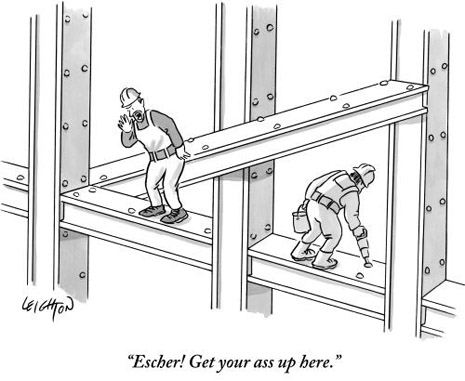
\includegraphics[width=8cm]{cartoon3.png}
\end{center}


\sektion{Foundations of Analysis}
\begin{quote}
If you really understood this course, you won't need to do any revision. Just relax and have some beer. 
\begin{flushright}
      \textit{ -  Alessio Corti}
       \end{flushright} 
\end{quote} \vspace*{5pt}

\subsektion{The Completeness Axiom}\vspace*{5pt}
\begin{definition}
Let $\emptyset \neq S \subset \RR$. Any element $x \in S$ is the \emph{maximum} of $S$:
\[x = \max S\text{ if }\forall y \in S,~y \leq x\]
Similarly $x \in S$ is the \emph{minimum} of $S$	
\[x = \min S\text{ if }\forall y\in S,~x \leq y\]
\end{definition}\vspace*{5pt}

It makes sense to call it \emph{the} maximum as there can only be one.\vspace*{5pt}

\begin{remark}
If $\emptyset \neq S \subset \RR$ then let $\phi \neq -S = \{-x ~|~ x \in S\}\subset \RR$, $\min S = -\max(-S)$. 	
\end{remark}\vspace*{5pt}
\begin{warning}
Make sure $S \neq \emptyset$, as the empty set has no maximum. 	
\end{warning}\vspace*{10pt}


\begin{examples}
\begin{enumerate}
\item $S = \{x ~|~ x \geq 0\}$
then $S$ has no maximum, min\,$S = 0$.

\item $S = (0,1)$
We would like to say that $1$ is the max, but this is not true because $1 \not \in S$. So $S$ has no maximum. $S$ has no min either. Clearly $x = 1$ is an ``important'' number for the set $(0,1)$. The next few definitions address this. 	
\end{enumerate}
\end{examples}\vspace*{5pt}


\begin{definition}
$\emptyset \neq S \subset \RR$ is \emph{bounded above} if 
\[\exists M \iR \text{ s.t. } \forall x \in S,~x \leq M\]
such an $M$ is called an \emph{upper bound} for $S$. 

$S$ is \emph{bounded below} if
\[\exists M \in \R \text{ such that } \forall x \in S, M \leq x\]
Such an $M$ is called a \emph{lower bound}.

$S$ is \emph{bounded} if $S$ is \emph{bounded above} and \emph{below}. 
\end{definition}\vspace*{5pt}

Equivalently $S$ is bounded if 
\[\exists R >0 \text{ such that } \forall x \in S, -R \leq x \leq R\]
or equivalently 
\[\exists R >0 \text{ such that } \forall x \in S, |x| \leq R\]\vspace*{2pt}

\begin{examples}~
$S = \{x \iR ~|~ x \geq 0\}$ is bounded below but not above. 

$S = \{x \iR ~|~ x \leq 0\}$ is bounded above, not below. 

$S = (0,1) = \{x \iR ~|~ 0 < x < 1\}$ is bounded (above and below). 	
\end{examples}\vspace*{5pt}

\begin{definition}
Suppose $\emptyset \neq S\subset \R$ is bounded above. The \emph{least upper bound} of $S$ a.k.a. the ``sup" (\emph{supremum}) of $S$, is the smallest of all upper bounds (assuming that it exists!), i.e.
 \[x = \mathrm{sup}\, S = \min T\text{ where }\emptyset \neq T = \{y ~|~ y \text{ is an upperbound for } S\}\]
 
 Similarly the \emph{greatest lower bound} of $S$, or ``inf" (\emph{infimum}) is the largest of all lower bounds (assuming that it exists!) i.e. 
 \[x = \mathrm{inf}\, S = \max T\text{ where }\emptyset \neq T = \{y~|~ y \text{ is a lower bound for } S \}\]
\end{definition}\vspace*{5pt}

\begin{example}
$S = (0,1)$. Then $T = \{y ~|~ y \text{ is an upperbound for } S\}$. 

$T$ has a minimum: $1 = \min T = \mathrm{sup}\, (0,1)$. Similarly $0 = \mathrm{inf}(0,1)$. 
\end{example}\vspace*{5pt}


\begin{axiom}[Completeness of $\RR$]
Suppose that $\emptyset \neq S \subset \RR$ is bounded above. Then $S$ has a supremum.
\end{axiom}

This is an article of faith about the real numbers. There are very strange things that I would like to discuss that I won't tell you as I don't want to scare your innocent minds.

 You may want to use set theory to construct the real numbers and prove that the completion axiom is a theorem there. But what's worse is that if you study logic carefully, then you cannot state this axiom in ``first order logic", but I'm not going to go there; it's something that bothers me but it shouldn't bother you. \emph{Just believe it.}\\


Consequence: If $\emptyset \neq S \subset \R$ is bounded below then $S$ has an inf. Indeed: $S$ is bounded below $\implies -S$ is bounded above and inf $S=- \mathrm{sup}(-S)$.\\

\emph{Exercise.} Prove that there is a real number $x \iR$ such that $x^2 = 2$. In other words, $\sqrt{2}$ exists as a real number. 

Hint: \begin{enumerate}
 \item Let $r = \sup\,\{x \iR ~|~ x^2 < 2\}$. You next try to show $r^2 = 2$. To do that the following characterisation of sup $S$ may help. 
 \item $L = \mathrm{sup}\,S$ iff 
 \begin{enumerate}
 \item $L$ is an upperbound ($\forall x \in S,\, x \leq L$)
 \item $\forall \epsilon >0, \epsilon \iR$, $\exists \, x \in S$ such that $L-\epsilon < x$
 \end{enumerate}
 \end{enumerate}\vspace*{10pt}


So \lecturemarker{27}{blah}
I introduced sup $S$ for $\emptyset \neq S \subset \R$ bounded above: 
\[
\begin{aligned}
  \mathrm{sup}\,S &= \min\{ t\iR: t \text{ an upper bound for } S\}\\
  &= \min\{t \iR ~|~ \forall x \in S, x \leq t\}
\end{aligned}
\]

\textbf{Criterion to help recognising sup $S$}

$L = \sup\,S$ if and only if
\begin{enumerate}
\item[(1)] $L$ is an upper bound for $S$, i.e. $\forall x \in S, x \leq L$.
\item[(2)] $\forall \epsilon >0, \exists x \in S$ such that $L-\epsilon <x$.
\end{enumerate}\vspace*{5pt}

I think the idea is easy to understand: 

\begin{center}
\begin{tikzpicture}[scale=5, node distance=2cm]
\draw[latex-latex] (-0.5,0) -- (1.5,0) ; %edit here for the axis
\draw[shift={(0.75,0)},color=black] (0pt,0pt) -- (0pt,-1pt) node[above, yshift=0.3cm] 
{$x \in S$};
\draw[shift={(0.6,0)},color=black] (0pt,1pt) -- (0pt,-1pt) node[above, yshift=-0.5cm] 
{$L-\epsilon$};
\draw[shift={(1,0)},color=black] (0pt,1pt) -- (0pt,-1pt) node[above, yshift=-0.5cm] 
{$L$};
%\draw[*-o] (0.92,0) -- (2.08,0);
\draw[very thick] (0.6,0) -- (1,0);
\end{tikzpicture}%picture of line
\end{center}

Think: $\epsilon$ is \emph{small}, then $L-\epsilon$ is a little bit smaller than $L$; then (2) is just saying that $L-\epsilon$ is not an upperbound for $S$. 

[Recall that $M$ is an upperbound for $S \iff \forall x \in S, x \leq M$. $M$ is not an upperbound for $S \iff \exists x \in S$ such that $M < x$]

Equivalent formulation of (2) is 
\[\forall \epsilon > 0,\, L-\epsilon \text{ is not an upper bound for } S\]
also equivalent
\[(2\dagger) \quad \forall L', L'<L, L' \text{ is not an upper bound for } S.\]

\begin{proof}[Proof of the Criterion]
	Suppose that $L$ is sup $S$. Then (1) is obvious (the min of a set by definition belongs to that set.)
	
(2) is done by the definition of min: If $L'$ is an upper bound $\implies L \leq L'$, or equivalently $L'$ is not an upperbound $\impliedby L' <L$. This shows that $(2\dagger)$ holds, hence (2) holds. 
	
	For the converse, suppose that (1) and $(2\dagger)$ hold. I want to show $L =$ sup $S$. i.e. $L = \min T$, where $T = \{t \iR ~|~ t \text{ an upper bound of } S$. (1) is saying $L \in T$. $(2\dagger)$ is saying $L' \in T \implies L \leq L'$. i.e. indeed $L = \min T$.
\end{proof}

Application: 
\begin{theorem}[Existence of Square-Root]
$\forall y \iR, y \geq 0,\,\exists! x \iR, x \geq 0\text{ such that }x^2 =y$.
\end{theorem}\vspace*{5pt}

\begin{remark}~\\[-0.5cm]

(1) $x = \sqrt{y}$. This shows the existence of the square-root function.

(2) Using the same ideas, you can show $\forall n \geq 2, n \iN:$
\[\forall y\iR, y\geq 0, \exists! x \iR, x\geq 0 \text{ such that } x^m = y\]	
(i.e. the existence of the $n$-th root function.)
\end{remark}

\begin{proof}
We are supposed to do this using sup. 

Fix  $y \geq 0$. Let $x = \mathrm{sup}\,\{t \geq 0~|~ t^2 \leq y\}$. In order for this to make sense, we need to check that $T = \{t \geq 0~|~ t^2 \leq\}$ is bounded above. [$0 \in T$, so $T \neq \emptyset$]

Indeed $M = \max\{1,y\}$ is an upper bound for $T$. (think about this as an exercise). 

\textbf{Claim.} $x^2 =y$. 

Step 1: $x^2 \leq y$. I want to use property (2) of the criterion for sup. If $x'$ is a little smaller than $x$ then $x'$ is not an upperbound for $T$. So \[\exists t \in T: x' < t \implies x'^2 < y^2 \leq y.\] So again: $\forall x', x'< x \implies x'^2 \leq y$. In other words, $\forall \epsilon >0,\,(x-\epsilon)^2 \leq y$
\[\begin{aligned}
\implies x^2 - 2\epsilon \leq (x-\epsilon)^2 &= x^2 - 2\epsilon x + \epsilon^2 \leq y	
\end{aligned}\]
i.e. 
$\forall \epsilon >0:$
\[x^2 \leq y + 2\epsilon x \leq y + 2M\epsilon\]

\emph{Exercise:} Let $x_1,x_2 \iR, A >0$. Suppose $\forall \epsilon >0, x_1\leq x_2 + A\epsilon$. Then $x_1 \leq x_2$. 

Once you've done this, you will have shown $x^2\leq y$ i.e. Step 1.\\ 

Step 2: $y \leq x^2$. We take this back to property (1) of the criterion for sup. $x$ is an upper bound for $T = \{ t ~|~ t^2 \leq y\}$. 

Suppose for contradiction $x^2 < y$. Then I claim $x$ is not an upper bound for $T$, i.e. 
\[\exists \epsilon >0 \text{ such that } x + \epsilon \leq T\]
i.e. 
\[\exists \epsilon >0 \text{ such that } (x+\epsilon)^2 <y\]
In other words:
\[\text{If } x^2 < y, \text{ then }\exists \epsilon >0 \text{ such that } (x+\epsilon)^2 < y\]

Compute
\[(x+\epsilon)^2 = x^2 + 2\epsilon x + \epsilon^2\]
provided that I choose my $\epsilon$ to be $\leq 1$, this is $\leq x^2 + 2\epsilon x + \epsilon = x^2 + \epsilon(2x + 1)$. 

Formally, I choose: 
\[0 < \epsilon < \min\left\{1,\frac{y-x^2}{2x+1}\right\}\]
then I claim $(x+\epsilon)^2 < y$ (and this finishes the proof). 

Indeed: 
\begin{align*}
  (x+\epsilon)^2 &= x^2 + 2\epsilon x + \epsilon\\
  &\leq x^2 + 2\epsilon x + \epsilon \\
  &= x^2 + \epsilon (2x + 1)\\
  &< x^2 + \frac{y-x^2}{2x+1}2x+1 = y\qedhere
\end{align*}
\end{proof}\vsp

\subsektion{* Sequences and Limits *}
\emph{The}\lecturemarker{31}{blah} \emph{rest of these notes are unexamined in M1F (but are in M1P1, where it's recovered).}\\

\begin{definition}
A \emph{sequence} of real numbers is an infinite list of real numbers: 
\[a_1,a_2,a_3,\dots,a_n,\dots\]	
one for each positive integer $n$.
\end{definition}

\textbf{Notation.} We denote a sequence $(a_n)_{n \iN^{\times}}$, or just $(a_n)$. 

Note the ``round" parentheses $(,)$ to distinguish from the notation for sets that uses $\{,\}$ curly brackets.\vspace*{5pt}

\begin{remark}
A sequence is a function $a: \N^\times \to \R$ with $a(n) = a_n$. 	
\end{remark}\vspace*{5pt}


\begin{examples}
\begin{enumerate}
\item $1,\frac{1}{2},\frac{1}{3},\frac{1}{4},\dots,\frac{1}{n},\dots$
\[a_n = \frac{1}{n}\]

\item $1,0,1,0,1,0,1,\dots$
\[a_n = \frac{1-(-1)^n}{2} = \begin{cases}
1 \mbox{ if $n$ is odd}\\
0 \mbox{ if $n$ is even}	
 \end{cases}
\]	
	
\item $1,1,2,3,5,8,\dots$ - the Fibonacci sequence. 

The easiest way to define this is by induction:
\[\begin{cases}
a_1 &= a_2 = 1\\
a_n &= a_{n-1} + a_{n-2} \quad \text{ for } n \geq 3	
\end{cases}
\]
\item $1,1 + \frac{1}{2}, 1 + \frac{1}{2}+ \frac{1}{3},\dots$. 
\[a_n = \sum_{k=1}^n \frac{1}{k}\]
\item $\frac{1}{2},\frac{2}{3},\frac{3}{4},\frac{4}{5},\dots$
\[a_n = \frac{n}{n+1}\]
\end{enumerate}
\end{examples}

I want to define the notion of a limit of a sequence ($a_n$) as $n \to \infty$. (``$n$ tends to $\infty$")\vspace*{5pt}

\textbf{A little preparation}

Here $l \iR, \epsilon >0$. The statement $|x-l|<\epsilon$ means ``$x$ is within $\epsilon$ of $l$", i.e.
\[-\epsilon < x-l<\epsilon \iff l-\epsilon < x < l + \epsilon\]

in other words $x \in$ open window of radius $\epsilon$ centred at $l$. I picture this: 

\begin{center}
\begin{tikzpicture}[scale=5, node distance=2cm]
\fill[blue!20] (0.4,-0.02) rectangle (0.8,0.02);
\draw[latex-latex] (-0.5,0) -- (1.5,0) ; %edit here for the axis
\draw[shift={(0.6,0)},color=black] (0pt,1pt) -- (0pt,-1pt) node[above, yshift=0.3cm] 
{$l $};
\draw[shift={(0.4,0)},color=black] (0pt,1pt) -- (0pt,-1pt) node[above, yshift=-0.5cm] 
{$l-\epsilon$};
\draw[shift={(0.8,0)},color=black] (0pt,1pt) -- (0pt,-1pt) node[above, yshift=-0.5cm] 
{$l+\epsilon$};
\node at (1.5,-0.07) {$\R$};
%\draw[*-o] (0.92,0) -- (2.08,0);
%\draw[very thick] (0.92,0) -- (1.92,0);
\end{tikzpicture}%picture of line
\end{center}


\begin{definition}
Let $(a_n)$ be a sequence and $l \iR.$ I say that $a_n \to l$ (``$a_n$ tends to $l$") as $n \to \infty$ and I write this as $\lim_{n \to \infty} a_n = l$ iff: 
\[\forall \epsilon >0,\, \exists N \iN\text{ such that } n \geq N \implies |a_n - l| < \epsilon\]
\end{definition}

Intuitively: If $n$ is large, then $a_n$ is very close to $l$.\\


\begin{example}
$a_n = \frac{1}{n} \to 0$ as $n \to \infty$
\begin{proof}
Fix $\epsilon >0$.

Let $N$ be any integer such that $N > \frac{1}{\epsilon}$. (we know such $N$ exists by the Archimedean axiom.) If $n \geq N$ then 
\[|a_n - 0| = \frac{1}{n} \leq \frac{1}{N} <\epsilon\]
\end{proof}
\end{example}\vspace*{5pt}

\begin{example}
Let $a_n = \dfrac{1-(-1)^n}{2}$, i.e. $a_n = \begin{cases}
 1 \mbox{ if $n$ is odd}\\
 0 \mbox{ if $n$ is even}	
 \end{cases}$
 
 This sequence tends to \emph{no limit}. 
 
 This is rather awkward to prove directly from the definition, becuase you would have to show 
 \[\forall l \iR,\, \exists >0 \forall N, \exists n \geq N\text{ s.t. } |a_n - l| \geq \epsilon\]
 But you try. You'll then see there are tricks that allow you do this more efficiently. Indeed the thing I do next will help you prove this directly. 
\end{example}\vspace*{5pt}



\begin{proposition}[Uniqueness of limits]
Let $(a_n)$ be a sequence. Suppose $l_1 = \lim_{n \to \infty} a_n$ and	$l_2 = \lim_{n \to \infty} a_n$. Then $l_1 = l_2$.
\end{proposition}

Picture of proof: 

\begin{center}
\begin{tikzpicture}[scale=5, node distance=2cm]
\fill[blue!20] (0.6,-0.02) rectangle (1,0.02);
\fill[red!20] (-0.1,-0.02) rectangle (0.3,0.02);
\draw[latex-latex] (-0.5,0) -- (1.5,0) ; %edit here for the axis
\draw[shift={(0.8,0)},color=black] (0pt,1pt) -- (0pt,-1pt) node[above, yshift=0.3cm] 
{\small $l_2$};
\draw[shift={(0.6,0)},color=black] (0pt,1pt) -- (0pt,-1pt) node[above, yshift=-0.5cm] 
{\small $l_2-\epsilon$};
\draw[shift={(1,0)},color=black] (0pt,1pt) -- (0pt,-1pt) node[above, yshift=-0.5cm] 
{\small$l_2+\epsilon$};

\node at (1.5,-0.07) {$\R$};
\begin{scope}[shift={(-.5,0)}]
\draw[shift={(0.6,0)},color=black] (0pt,1pt) -- (0pt,-1pt) node[above, yshift=0.3cm] 
{\small $l_1$};
\draw[shift={(0.4,0)},color=black] (0pt,1pt) -- (0pt,-1pt) node[above, yshift=-0.5cm] 
{\small $l_1-\epsilon$};
\draw[shift={(0.8,0)},color=black] (0pt,1pt) -- (0pt,-1pt) node[above, yshift=-0.5cm] 
{\small $l_1+\epsilon$};	
\end{scope}
\end{tikzpicture}%picture of line
\end{center}

We pick $\epsilon < \frac{l_2-l_1}{2}$. Then the windows $(l_1-\epsilon,l_1+\epsilon)$ and $(l_2-\epsilon,l_2+\epsilon)$ are disjoint, however $\exists N$ such that $n \geq N \implies a_n$ has to go in both windows, a contradiction.


\begin{proof}
Fix $\epsilon >0$. By the definition of a limit 
\[\exists N_1 \text{ such that } n \geq N_1 \implies |a_n - l_1| <\epsilon/2\]	
\[\exists N_2 \text{ such that } n \geq N_2 \implies |a_n - l_2| <\epsilon/2\]	

Consider $N = max\{N_1,N_2\}$. If $n \geq N \implies |a_n - l_1| < \epsilon/2$ and $|a_n - l_2| <\epsilon/2$. 

Now look at this: 
\[
\begin{aligned}
  |l_1 - l_2| &= |l_1 - a_n + a_n - l_2|\\
  &\leq |a_n - l_1| + |a_n - l_2|\\
  &< \epsilon /2 + \epsilon/2 =\epsilon 
\end{aligned}
\]

So $|l_1 - l_2| < \epsilon \implies |l_1 - l_2| = 0$, i.e. $l_1 = l_2$. 
\end{proof}


\textbf{Strategy to prove $a_n \to l$ directly}\lecturemarker{32}{blah}

Step 1: Fix $\epsilon >0$. 

Step 2: Compute $|a_n - l|$

STEP 3: Solve (for $n$) the inequality $|a_n - l| < \epsilon$. 

Step 4: Choose $N \iN$ such that $n \geq N \implies |a_n - l| < \epsilon$	

Step 5: Turn this ``upside down" and write your own proof.\\

\textbf{Felina.} Finally we will show the limits of two sequences: 
\[(1)\; a_n= \dfrac{n+5}{n+1} \to 1 \quad (2)\; a_n = \dfrac{n^2 - 5}{n^3-50} \to 0\]

It's blindingly obvious that this is the limit, and no one in their right mind would spend a fraction of their life thinking about it.	Similarly for the second example, the $-5$ is just a red herring, $-50$ is just some bullshit; I could have put $5$ billion or whatever, it doesn't matter.

 You might think this is the educational equivalent of sadism - I keep this dungeon with lots and lots of questions like this, which I use to torment you! That's not the real purpose; I'm not a sadist, believe it or not. But it's to develop a skill, to write a precise mathematical argument, and develop a greater control of your thought processes, it's a kind of yoga of the brain, not the body. At the beginning when you go to yoga class you don't do those amazing things you see when you open up a yoga master book. It will take some time and training, and in yoga 101 you do some pretty stupid things, and it's the same with maths. It's a bit silly, this is  not a problem about sequences, but it does develop the skill. That's why you do it.\\


\begin{example}
Show $a_n= \dfrac{n+5}{n+1} \to 1$.


\emph{Rough work.} 
Step 1: Fix $\epsilon >0$. 

Step 2: Calculate $|a_n-l|$
\[
\begin{aligned}
  |a_n - l| &= \frac{n+5}{n+1} - 1 = \frac{n+5-n-1}{n+1}\\
  &= \frac{4}{n+1}
\end{aligned}
\]

STEP 3: solve for $n$ $|a_n - l| < \epsilon$. 
\[
\begin{aligned}
  \frac{4}{n+1} < \epsilon &\iff 4 < \epsilon(n+1)\\
  &\iff n_1 > \frac{4}{\epsilon}\\
  &\iff n > \frac{4}{\epsilon} -1
\end{aligned}
\]


Step 4: If $N = \lceil \frac{4}{\epsilon} -1\rceil + 1$, then $n \geq N \implies |a_n -l| < \epsilon$.\vspace*{5pt}

(\textbf{Notation:} if $\alpha \in \R$, than $\lceil \alpha\rceil =$ \emph{round up} of $x = \min \{k\iZ ~|~ k \geq \alpha\})$

Step 5: Turn this into a proof. 

\begin{proof}
Fix $\epsilon >0.$ Let $N = \lceil \frac{4}{\epsilon} -1\rceil +1$. Now if $n \geq N$, then 
\begin{align*}
  n > \frac{4}{\epsilon} - 1 &\implies n + 1> \frac{4}{\epsilon}\\
  &\implies \frac{4}{n+1} = |a_n - l| < \epsilon.\qedhere
\end{align*}
\end{proof}
\end{example}\vspace*{5pt}

	
	
\begin{example} Show that $a_n = \dfrac{n^2 - 5}{n^3-50} \to 0$.\\
	
	
	\emph{Rough work.} We want to prove that $a_n \to 0$. Compute: 
	\[|a_n - l| = \frac{|n^2- 5|}{|n^3 - 50|}\]
	It is going to be awkward to solve for $n$: 
	\[\frac{|n^2- 5|}{|n^3 - 50|} < \epsilon\]
	

	We need to modify STEP 3 and 4: 
	
	(2$\frac{1}{2}$) Find $b_n \geq 0$ and $n_0 \iN$ such that $n \geq n_0 \implies |a_n -l| \leq b_n$. 
	
	(3') Solve for $n$, $b_n < \epsilon$.
	
	(4') Choose $N \geq n_0 \in \Z$ such that $n \geq N \implies b_n <\epsilon$. 
	
	(5) Turn this upside down and write your proof.\\
	
	\textbf{Let's try this:}
	
	(2$\frac{1}{2}$) Choose $b_n$, now $|a_n -l| = \left|\dfrac{n^2-5}{n^3-50}\right|$. I choose $b_n = \frac{2}{n}$.
	
	 I need $n_0$ such that $ \left|\dfrac{n^2-5}{n^3-50}\right| \leq b_n$ for all $n \geq n_0$. 
	
	$n_0 \geq 3$, so numerator is positive. We want $n^3 - 50 \geq \frac{n^3}{2}$. 
	
	Note: If $n \geq 4$ then both the numerator $n^2 -5 >0$ and the denomiator $n^3 - 50 > 0$. I am definitely going to take $n_0 \geq 4$, so 
	\[\left|\frac{n^2-5}{n^3-50}\right| = \frac{n^2-5}{n^3-50}\]
	and then I want to fix 
	\[\frac{n^2-5}{n^2-50}\leq \frac{n^2}{n^3-50}\leq \frac{2}{n}\]
	i.e. $n^3 \leq 2(n^3-50)$. It's enough that $100 \leq n^3$, i.e. OK for $n \geq 5$. 
	
	Message: For $n_0 = 5, \left|\frac{n^2-5}{n^3-50}\right| \leq \frac{2}{n}$. To wrap this up, take $b_n = \frac{2}{n}$ and $n_0 = 5$.\\
	
	(3') $b_n < \epsilon: \frac{2}{n} < \epsilon \iff n >\frac{2}{\epsilon}$. 
	
	(4') Let $N = \lceil \frac{2}{\epsilon}\rceil + 1$.	
	
	Now we're ready to put everything together into a proof: 
	
	\begin{proof} Fix $\epsilon > 0$. Let $N = \max\{\lceil \frac{2}{\epsilon} \rceil + 1,\;5\}$.
	
	\textbf{Claim:} If $n \geq 5$, then $|a_n - l| \leq 2/n$.
	
	\textit{Proof of Claim.}
	\[
	\begin{aligned}
|a_n - l| &= \frac{|n^2-5|}{|n^3-50|} = \frac{n^2 - 5}{n^3-50} \\
& \leq \frac{n^2}{n^3/2} = 2/n ~//	
\end{aligned}
\]	
by the claim, if $n \geq N$, then 
\[|a_n - l| \leq \frac{2}{n} < \frac{2}{2/\epsilon} = \epsilon \qedhere\]
\end{proof}
\end{example}

  
\theend 

\end{document}
	





